% !TEX root = ./thesis.tex
%
% thesis.tex
% Beyond Scalar Fitness: Behavioural Feedback for LLM-Driven Metaheuristic Evolution
% Max Harell, LIACS, Leiden University
%

\documentclass[10pt,a4paper,twocolumn]{article}

% ---------- Page layout ----------
\usepackage[left=1.7cm,right=1.7cm,top=2cm,bottom=2.3cm,columnsep=0.7cm]{geometry}

% ---------- Typography ----------
\usepackage{microtype}
\usepackage[T1]{fontenc}
\usepackage{lmodern}
\frenchspacing
\setlength{\parindent}{1em}
\setlength{\parskip}{0pt}

% ---------- Reduce whitespace around figures ----------
\setlength{\textfloatsep}{8pt plus 2pt minus 2pt}
\setlength{\floatsep}{6pt plus 2pt minus 2pt}
\setlength{\intextsep}{6pt plus 2pt minus 2pt}
\setlength{\abovecaptionskip}{4pt}
\setlength{\belowcaptionskip}{2pt}

% ---------- Section formatting ----------
\usepackage{titlesec}
\titleformat{\section}{\large\bfseries}{\thesection}{1em}{}
\titleformat{\subsection}{\normalsize\bfseries}{\thesubsection}{1em}{}
\titleformat{\subsubsection}{\normalsize\itshape}{\thesubsubsection}{1em}{}
\titlespacing*{\section}{0pt}{1.8ex plus 0.5ex}{0.8ex plus 0.2ex}
\titlespacing*{\subsection}{0pt}{1.2ex plus 0.3ex}{0.5ex plus 0.1ex}
\titlespacing*{\subsubsection}{0pt}{1.0ex plus 0.2ex}{0.4ex plus 0.1ex}

% ---------- Math ----------
\usepackage{amsmath}
\usepackage{amssymb}

% ---------- Non-floating captions ----------
\usepackage{caption}

% ---------- Graphics and tables ----------
\usepackage{graphicx}
\usepackage{subcaption}
\usepackage{booktabs}
\usepackage{xcolor}
\usepackage{float}

% ---------- Algorithms ----------
\usepackage[ruled,vlined,linesnumbered]{algorithm2e}

% ---------- Code listings ----------
\usepackage{listings}
\lstset{
  basicstyle=\ttfamily\footnotesize,
  breaklines=true,
  frame=single,
  numbers=left,
  numberstyle=\tiny\color{gray},
  captionpos=b,
}

% ---------- Cross-references ----------
\usepackage[
  setpagesize=false,
  colorlinks=true,
  linkcolor=black,
  citecolor=blue!60!black,
  urlcolor=blue!60!black,
  pdftitle={Beyond Scalar Fitness: Behavioural Feedback for LLM-Driven Metaheuristic Evolution},
  pdfauthor={Max Harell}
]{hyperref}
\usepackage[capitalise,noabbrev]{cleveref}

% ---------- Compact lists ----------
\usepackage{enumitem}
\setlist{nosep,leftmargin=1.5em}

% ---------- Section numbering ----------
\setcounter{secnumdepth}{3}

% ---------- Remap chapter hierarchy for article class ----------
\let\chapter\section
\let\section\subsection
\let\subsection\subsubsection
\let\subsubsection\paragraph

% ==========================================================================
\begin{document}

% ---------- Title block ----------
\twocolumn[{%
\begin{center}
\vspace*{0.2cm}
{\LARGE\bfseries Beyond Scalar Fitness:\\[0.3em]
Behavioural Feedback for LLM-Driven\\Metaheuristic Evolution\par}
\vspace{0.7cm}
{\large Max Harell\par}
\vspace{0.15cm}
{\small LIACS, Leiden University, The Netherlands\par}
\vspace{0.5cm}
{\small Bachelor Thesis in Computer Science\par}
{\small Supervised by Dr.\ Niki van Stein\par}
\vspace{0.15cm}
{\small \today\par}
\vspace{0.6cm}
\end{center}

\begin{center}
\begin{minipage}{0.92\textwidth}
\small
\noindent\textbf{Abstract.}\quad The LLaMEA framework embeds a large language model in an evolutionary loop to generate optimisation algorithms, with the Area Over the Convergence Curve (AOCC), a single scalar value, as its only feedback signal. Recent work has shown that augmenting feedback with structural features extracted from the algorithm's source code improves performance, but the analogous question for \emph{behavioural} features (descriptors of the search trajectory the algorithm produces when it runs) has remained open. This thesis addresses that question through a four-stage pipeline. Stage one screens ten LLMs and identifies Gemini 3 Flash as the strongest combination of quality, reliability, and cost. Stage two reduces a 32-feature behavioural vocabulary to a tractable subset of ten via tri-criterion consensus. Stage three compares neutral, directional, and comparative framings of each behavioural feature on Gemini 3 Flash across 29 conditions. Stage four is a head-to-head full-benchmark comparison of behavioural, structural (LLaMEA-SAGE), and combined feedback against vanilla AOCC-only on a 20-function MA-BBOB set with 10 seeds per condition. We find that neutral framing of behavioural features, reporting the feature value without prescriptive advice, consistently outperforms the prescriptive variants, and that prescriptive feedback steers the median feature value in the advised direction in only 37\% of cases despite empirically grounded advice. On the stage four benchmark, all three feedback-augmented conditions outperform vanilla LLaMEA with the decisive effect being variance reduction. Combined behavioural and structural feedback shrinks seed-to-seed standard deviation by roughly a factor of five (Levene $p = 0.030$, the only Stage~4 contrast to clear $\alpha = 0.05$), and the three feedback conditions split 19 of 20 leaderboard wins between them. Re-evaluated on the full $1{,}000$-instance MA-BBOB pool, all four LLM-generated winning algorithms outperform a CMA-ES baseline across $d \in \{5, 10, 20\}$. Trajectory-based behavioural feedback does guide LLMs to design better optimisation algorithms, but the improvement manifests primarily as reduced failure-mode variance rather than as a large mean performance lift.
\end{minipage}
\end{center}
\vspace{0.6cm}
}]

% ---------- Content ----------
% !TEX root = ../thesis.tex
% =============================================================================
% Chapter 1: Introduction
% =============================================================================

\chapter{Introduction}
\label{ch:introduction}

Designing effective optimisation algorithms is hard. Decades of research have produced hundreds of metaheuristic strategies, each with its own strengths, parameters, and failure modes~\cite{eiben2015introduction}. Selecting or configuring the right algorithm for a given problem remains a largely manual process guided by researcher intuition, despite substantial progress in automated algorithm configuration~\cite{hutter2009paramils} and selection~\cite{rice1976algorithmselection}.

Large Language Models (LLMs) have introduced a fundamentally new paradigm for algorithm design. Rather than searching within a predefined space of modules or parameters, LLMs can generate complete optimisation algorithms as executable code by leveraging ideas from the vast body of algorithmic knowledge encoded in their training data. The LLaMEA framework~\cite{vanStein2024LLaMEA} embeds an LLM within an evolutionary loop. It generates candidate algorithms, evaluates them on benchmark problems, and uses the performance feedback to guide subsequent generations. On standard benchmarks, LLaMEA-generated algorithms rival or surpass established metaheuristics like CMA-ES~\cite{hansen2001cmaes}.

In the standard LLaMEA loop the sole feedback signal to the LLM is the Area Over the Convergence Curve (AOCC)~\cite{vanStein2024LLaMEA}, a scalar performance score. While AOCC captures anytime performance, it compresses the entire optimisation trajectory, spanning thousands of evaluations across multiple problem instances, into a single number. Two algorithms with identical AOCC scores may exhibit fundamentally different search behaviours. One might converge quickly through aggressive exploitation, while another might explore broadly before settling on a good solution.

The BLADE benchmarking suite ~\cite{vanStein2025BLADE} captures algorithmic behaviour by storing the algorithm's execution trajectory. Behavioural features extracted from these trajectories can quantify exploration breadth, exploitation intensity, convergence speed, step-size dynamics, and stagnation patterns. Prior work has shown that these features explain why certain LLM-generated algorithms outperform others ~\cite{vanStein2025Behaviour}, and that structural code features can successfully guide the algorithm design process when fed back as natural-language instructions~\cite{vanStein2026LLaMEASAGE}.

The question this thesis addresses is whether behavioural features, which describe what the algorithm \emph{does} rather than what it \emph{is}, can play a similar guiding role. Answering it raises three interrelated questions: which LLMs are capable enough to generate high-quality algorithms in the first place, which behavioural features actually carry information about algorithm quality, and whether the \emph{framing} of that feedback matters to the LLM.

The following research question and sub-questions guide the exploration of this thesis,

\medskip

\begin{description}[leftmargin=4.5em, labelwidth=3.7em, labelsep=0.6em, itemsep=0.45em, align=left, font=\normalfont\bfseries]
  \item[RQ.] \itshape Can trajectory-based behavioural feedback guide LLMs to design better optimisation algorithms?
  \item[SubQ1.] \itshape Which LLMs can reliably generate high-quality metaheuristics for continuous black-box optimisation?
  \item[SubQ2.] \itshape Which trajectory-based behavioural features are most informative about algorithm quality?
  \item[SubQ3.] \itshape Does the framing of behavioural feedback (neutral observation, directional guidance, or comparative anchoring) affect the performance of LLM-generated algorithms?
\end{description}

\medskip

This thesis makes four contributions to the literature on LLM-driven automated algorithm design. The first is an extended behavioural feature set that grows the existing BLADE catalogue from 11 to 32 metrics. These span existing trajectory-based features adapted for this task~\cite{vanStein2025Behaviour,cenikj2023dynamorep,cenikj2026features}, information-theoretic inspired features that treat fitness longitudinally~\cite{richman2000sampen,bandt2002permutation,weinberger1990fitness,lempel1976complexity}, and six metrics entirely new to the optimisation literature~\cite{barabasi2005bursts}. The second is a multi-model screening of 10 LLMs, spanning 3B to 32B parameters across six model families plus two cloud API models, that identifies viable candidates for automated metaheuristic design. The third is evidence that the framing of behavioural feedback matters. Across 29 experimental conditions comparing neutral, directional, and comparative formats, neutral reporting (simply stating the behavioural observation without interpretation) consistently outperforms prescriptive formats that tell the LLM which direction is better. The fourth is a full-benchmark head-to-head comparison of behavioural, structural ~\cite{vanStein2026LLaMEASAGE}, and combined feedback against the vanilla AOCC-only baseline, which positions trajectory-based signals relative to the strongest existing alternative.

% !TEX root = ../thesis.tex
% =============================================================================
% Chapter 2: Background and Related Work
% =============================================================================

\chapter{Background and Related Work}
\label{ch:background}

% ---------------------------------------------------------------------------
\section{Metaheuristic Optimisation}
\label{sec:bg-metaheuristics}

A metaheuristic is a high-level, problem-independent strategy for solving optimisation problems of the form
\[
  \min \mathcal{F}(x), \qquad x \in \mathcal{S} \subseteq \mathbb{R}^d,
\]
where $x$ is a $d$-dimensional candidate solution, $\mathcal{S}$ is the bounded feasible search space, and $\mathcal{F}: \mathcal{S} \to \mathbb{R}$ is a black-box objective function that can be evaluated but whose gradient or structure is unknown~\cite{sorensen2013metaheuristics}. Metaheuristics work by iteratively generating, evaluating, and selecting candidate solutions according to heuristic rules that govern how the search space is explored. Unlike exact methods, they make no guarantees of optimality but can find good solutions efficiently across a wide range of problem types.

The field encompasses a broad family of algorithms. Evolution Strategies (ES) maintain a population of candidate solutions and apply Gaussian mutation with self-adaptive step sizes~\cite{back1996evolutionary}. CMA-ES extends this by learning a full covariance matrix that captures the local landscape geometry, and is widely considered the state of the art for continuous black-box optimisation~\cite{hansen2001cmaes}. Differential Evolution (DE) generates trial solutions by combining vector differences sampled from the current population~\cite{storn1997de}.

Despite their success, the design of metaheuristics remains largely a manual endeavour. A vast number of methods have been proposed, many with overlapping mechanisms and limited systematic benchmarking~\cite{aranha2022metaphor}. Choosing the right algorithm for a given problem, configuring its parameters, or designing a new variant requires deep expertise and extensive experimentation. This motivates the pursuit of automated, and increasingly explainable, approaches to algorithm design~\cite{vanStein2025Explainable}.

% ---------------------------------------------------------------------------

\section{Automated Algorithm Design}
\label{sec:bg-aad}

The automated design of optimisation algorithms has evolved through several paradigms, each expanding the scope of what can be automated. The earliest framing is algorithm selection. Rice~\cite{rice1976algorithmselection} formalises the task as learning a mapping from problem features to the best-performing algorithm, drawn from a fixed portfolio of candidates evaluated on a set of problem instances. Meta-learning approaches~\cite{smithmiles2009meta} build on this framework by using landscape features to predict algorithm performance.

Rather than selecting among fixed algorithms, algorithm configuration optimises the hyperparameters of a single algorithm. ParamILS~\cite{hutter2009paramils} applies iterated local search in parameter space, treating algorithm performance on a benchmark as a black-box function of its parameters. These methods can find configurations that substantially outperform defaults, but they operate within a fixed algorithmic structure.

Modular frameworks bridge selection and configuration by decomposing algorithms into interchangeable components. Van Rijn et al.~\cite{vanRijn2016modular} evolve the structure of evolution strategies by treating algorithmic modules (selection, recombination, mutation operators) as parameters of a meta-optimisation problem, and Vermetten et al.~\cite{vermetten2023modde} apply the same principle to DE. Such frameworks can search over millions of algorithm configurations, but they remain limited to the modules their designers included. The design space is large but bounded.

A broader methodology is proposed by Hoos~\cite{hoos2012pbo} under the banner of programming by optimisation. Rather than designing a single algorithm, developers should expose all design decisions as parameters and let automated methods search the resulting space. Genetic Improvement~\cite{petke2018gi} takes this further by applying evolutionary operators directly to source code, modifying and recombining program fragments to improve non-functional properties. These ideas foreshadow the shift to code-generation based approaches, where algorithms are constructed from scratch rather than configured from templates.

% ---------------------------------------------------------------------------
\section{LLMs for Algorithm Design}
\label{sec:bg-llm-aad}

The emergence of LLMs capable of generating complex code has introduced a qualitatively different approach to algorithm design. Rather than searching within a predefined design space, LLMs can generate complete algorithms as executable programs, unconstrained by modular templates. Building on existing taxonomies of LLM--EC integration~\cite{vanStein2024LLaMEA,chauhan2025ecllmsurvey}, we group the relevant literature by the role the LLM plays in the evolutionary loop.

Prompt optimisation applies evolutionary algorithms to optimise the prompts given to LLMs. EvoPrompt~\cite{guo2024evoprompt} uses genetic algorithms to evolve prompts, outperforming human-engineered alternatives. The Automated Prompt Engineer (APE)~\cite{zhou2023ape} takes a similar approach using Monte Carlo search. These methods optimise how we communicate with LLMs but do not use LLMs to generate algorithms directly.

Code generation embeds the LLM itself inside the evolutionary loop. FunSearch~\cite{romeraparedes2024funsearch} demonstrated that LLMs embedded in this way can discover novel mathematical results, generating Python programs for the cap-set problem that surpassed known bounds through a distributed island model with millions of LLM calls. Evolution of Heuristics (EoH)~\cite{liu2024eoh} applies a similar principle to combinatorial optimisation, treating candidate heuristics as individuals in an evolutionary population. Algorithm Evolution using Large Language Model (AEL)~\cite{liu2023ael} is a related approach from the same group. The Self-Taught Optimiser (STOP)~\cite{zelikman2024stop} demonstrates recursive self-improvement where the LLM-generated code is itself a prompt optimiser, creating a meta-learning loop.

Complete metaheuristic generation, the setting this thesis operates in, extends code generation from heuristic components to full algorithms. LLaMEA~\cite{vanStein2024LLaMEA} generates full Python classes with initialisation, state management, and search logic for continuous black-box problems, unlike EoH or AEL which generate small heuristic components for combinatorial problems. The framework combines in-context learning (the LLM sees previous algorithms and their scores) with an evolutionary loop that provides selection pressure. A follow-up work~\cite{vanStein2025Behaviour} extends LLaMEA by logging and analysing the behavioural profiles of generated algorithms, showing that higher-performing algorithms consistently exhibit more intensive exploitation behaviour and faster convergence across six LLaMEA configurations. However, this behavioural information is used only for post-hoc analysis, not as feedback to the LLM.

LLaMEA-SAGE~\cite{vanStein2026LLaMEASAGE} goes a step further by feeding structural information about the generated code back into the prompt. SAGE extracts features from the Abstract Syntax Tree (AST) of each algorithm (graph-theoretic metrics, code complexity measures, and structural statistics) stores them in an archive alongside fitness scores, and uses SHAP analysis~\cite{lundberg2017shap} on a surrogate model to identify which features most influence performance. The resulting guidance is translated into natural-language instructions (e.g., ``try decreasing the cyclomatic complexity'') that augment the mutation prompt, yielding faster convergence on MA-BBOB than vanilla LLaMEA.

Several recent approaches offer alternative search strategies over the same design space. MCTS-AHD~\cite{zheng2025mctsahd} replaces the evolutionary loop with Monte Carlo Tree Search, organising generated heuristics in a tree structure that balances exploration and exploitation. LLM-driven Heuristic Neighbourhood Search (LHNS)~\cite{xie2025lhns} abandons population-based evolution in favour of single-solution neighbourhood search with ruin-and-recreate operators. Both achieve competitive results on combinatorial benchmarks, demonstrating that the search strategy over LLM-generated code is itself an active research question.

% ---------------------------------------------------------------------------
\section{Benchmarking and Evaluation}
\label{sec:bg-benchmarking}

Rigorous benchmarking is essential for comparing generated algorithms and providing meaningful feedback to the LLM. The Black-Box Optimisation Benchmark (BBOB)~\cite{hansen2021coco} defines 24 noiseless test functions spanning five function groups (separable, moderate conditioning, high conditioning, multimodal with adequate structure, multimodal with weak structure). Many-Affine BBOB (MA-BBOB)~\cite{vermetten2023mabbob} extends this by constructing novel instances through affine combinations of BBOB functions, providing much greater instance diversity while preserving known landscape properties. MA-BBOB is the benchmark used in recent LLaMEA versions~\cite{vanStein2026LLaMEASAGE} and in this thesis.

The evaluation infrastructure underneath these benchmarks is IOHexperimenter~\cite{deNobel2024iohexperimenter}, which runs algorithms on benchmark functions, enforces budget limits, and logs full trajectories; IOHanalyzer~\cite{wang2022iohanalyzer} provides statistical analysis and visualisation of the logged data. BLADE~\cite{vanStein2025BLADE} builds on IOHexperimenter to provide a standardised evaluation framework specifically for LLM-driven algorithm design, including prompt management, candidate logging, and behavioural metric computation.

The primary performance signal used in this thesis is AOCC~\cite{vanStein2024LLaMEA}, an anytime performance metric that captures not just the final solution quality but the entire convergence trajectory. Unlike fixed-target metrics that measure time-to-threshold, AOCC rewards algorithms that converge quickly \emph{and} reach good final solutions. It is the standard performance metric in the BLADE framework (see \cref{eq:aocc} for the formal definition).

% ---------------------------------------------------------------------------
\section{Trajectory-Based Analysis of Metaheuristics}
\label{sec:bg-behaviour}

A growing body of work analyses algorithm behaviour through the lens of its search trajectory. Search Trajectory Networks (STNs)~\cite{ochoa2021stn} discretise the search space and represent trajectories as graphs, enabling visual comparison of algorithm dynamics. DynamoRep~\cite{cenikj2023dynamorep} uses trajectory-based population dynamics, specifically per-generation statistics of objective and position distributions, to classify optimisation problems. Kostovska et al.~\cite{kostovska2022trajectory} combine landscape features with algorithm-internal state variables (step size, covariance matrix) computed along trajectories for warm-started algorithm selection. Cenikj et al.~\cite{cenikj2026features} survey the broader meta-feature landscape spanning problem, trajectory, and algorithm-internal signals. Across this body of work, however, trajectory-based features have been used for algorithm selection and problem classification, not as feedback signals within an algorithm design loop.

% !TEX root = ../thesis.tex
% =============================================================================
% Chapter 3: Behavioural Feature Design
% =============================================================================

\chapter{Behavioural Feature Design}
\label{ch:features}

This chapter defines the behavioural feature set used throughout the thesis. \Cref{sec:features:principles} states the criteria that guided feature design and selection. The remaining sections present the 32 resulting features, organised by origin and function: inherited metrics, step-size and movement dynamics, information-theoretic measures, adapted population dynamics, and features new to the optimisation literature.

Every feature is computed from a single trajectory, the ordered sequence of candidate solutions that an algorithm evaluates together with their fitness values. Formally, a trajectory is a sequence $\{(x_t, y_t)\}_{t=1}^{T}$ where $x_t \in \mathbb{R}^d$ is the $t$-th candidate solution with decision variables $x_t^{(0)}, \ldots, x_t^{(d-1)}$, and $y_t = \mathcal{F}(x_t)$ is its fitness. The best-so-far fitness at evaluation~$t$ is denoted $f^*_t = \min_{s \le t} y_s$. Throughout this thesis, trajectories are collected over $T = 2{,}000 \times d$ evaluations in $d = 5$ dimensions with bounds $[-5, 5]$, giving $T = 10{,}000$ evaluations per trajectory.

% ============================================================================
\section{Design Principles}
\label{sec:features:principles}

Four criteria guided the selection and design of behavioural features.

\begin{enumerate}
  \item \textbf{Computational cheapness.} MA-BBOB evaluations already carry the bulk of experiment runtime. Behavioural features should add only a small fraction of additional expense.

  \item \textbf{Distinctness.} Each feature should capture a dimension of behaviour not already covered by other features.

  \item \textbf{Interpretability for LLM feedback.} Features are reported to the language model as part of the behavioural feedback string. They must therefore carry clear, concise semantics that an LLM can act on.

  \item \textbf{Discrimination.} Features should separate high-performing from low-performing algorithms. We quantify this via Spearman correlation ~\cite{spearman1904proof} with AOCC and Kolmogorov--Smirnov effect size ~\cite{kolmogorov1933} between the top-25\% and bottom-25\% candidates.
\end{enumerate}

% ============================================================================
\section{Existing BLADE Metrics}
\label{sec:features:blade}

BLADE~\cite{vanStein2025BLADE} ships with eleven behavioural metrics introduced by van~Stein et al.~\cite{vanStein2025Behaviour}. They fall into four functional categories covering exploration and diversity, exploitation and intensification, convergence, and stagnation. We define each metric formally below, using the trajectory notation from the start of the chapter.

\paragraph{\texttt{avg\_nearest\_neighbor\_distance}.}
For each evaluation $x_k$ (sampled every tenth step for efficiency), the Euclidean distance to its nearest neighbour among the $H = 1{,}000$ most recent prior evaluations:
\begin{equation}
\label{eq:avg_nn_dist}
  \text{ANN} = \frac{1}{|\mathcal{K}|} \sum_{k \in \mathcal{K}} \min_{\max(0,\, k-H) \le j < k} \lVert x_k - x_j \rVert,
\end{equation}
where $\mathcal{K} = \{1, 11, 21, \ldots\}$. Large values indicate the search covers new territory at each step. Small values indicate repeated returns to previously visited regions.

\paragraph{\texttt{dispersion}.}
The radius of the largest empty hypersphere that fits inside $\mathcal{S}$ without containing any evaluated point:
\begin{equation}
\label{eq:dispersion_formal}
  \mathrm{disp}(X) = \sup_{y \in \mathcal{S}} \min_{1 \le t \le T} \lVert y - x_t \rVert_2.
\end{equation}
In practice the supremum is approximated by drawing $N = 10{,}000$ points $z_i$ uniformly from $\mathcal{S}$ and computing
\begin{equation}
\label{eq:dispersion}
  \widehat{\mathrm{disp}}(X) = \max_{1 \le i \le N} \min_{1 \le t \le T} \lVert z_i - x_t \rVert_2,
\end{equation}
with nearest-neighbour queries accelerated by a KD-tree. Large values indicate that large regions of $\mathcal{S}$ remain unvisited. Lower values signal better search-space coverage.

\paragraph{\texttt{avg\_exploration\_pct}.}
For any finite set $S \subset \mathbb{R}^d$, the average pairwise Euclidean distance is
\begin{equation}
\label{eq:pairwise_dist}
  D(S) = \frac{2}{|S|(|S|-1)} \sum_{\substack{p < q \\ x_p, x_q \in S}} \lVert x_p - x_q \rVert_2.
\end{equation}
With axis widths $w_k = u_k - l_k$ and mean width $\bar{w} = \frac{1}{d}\sum_{k=1}^d w_k$, the expected pairwise distance of two i.i.d.\ uniform samples in $\mathcal{S}$ is approximated by
\begin{equation}
\label{eq:rand_div}
  D_{\mathrm{rand}} = \bar{w} \sqrt{d/6}.
\end{equation}
The trace $X$ is partitioned into $C$ consecutive chunks $S_0, \ldots, S_{C-1}$ of size $K = 500$, and each chunk is scored relative to random search:
\begin{equation}
\label{eq:chunk_exploration}
  E_c = \min\!\left\{100 \cdot \frac{D(S_c)}{D_{\mathrm{rand}}},\, 100\right\} \quad (0 \le E_c \le 100).
\end{equation}
The average exploration percentage is the mean across chunks:
\begin{equation}
\label{eq:avg_expl_pct}
  \bar{E} = \frac{1}{C} \sum_{c=0}^{C-1} E_c.
\end{equation}
Values near 100 indicate chunk-level diversity on par with random search. Values near 0 indicate concentrated, exploitative search.

\paragraph{\texttt{avg\_distance\_to\_best}.}
Let $b^*(k) = \arg\min_{t \le k} y_t$ denote the index of the best-so-far point at evaluation $k$. The mean distance from each evaluation to the best-so-far incumbent:
\begin{equation}
\label{eq:avg_dist_best}
  \bar{\Delta} = \frac{1}{T-1} \sum_{k=1}^{T-1} \lVert x_k - x_{b^*(k)} \rVert.
\end{equation}
Low values indicate strong local exploitation around the incumbent.

\paragraph{\texttt{intensification\_ratio}.}
The fraction of evaluations within a radius $r = 0.1 \cdot \bar{w}$ of the final best point $x^* = \arg\min_{t} y_t$:
\begin{equation}
\label{eq:intensification}
  I = \frac{1}{T} \sum_{t=1}^{T} \mathbf{1}\!\left[\lVert x_t - x^* \rVert < r\right].
\end{equation}
High values indicate strong exploitation near the eventual best solution.

\paragraph{\texttt{avg\_exploitation\_pct}.}
The complement of the exploration percentage:
\begin{equation}
\label{eq:avg_exploit_pct}
  \bar{X} = 100 - \bar{E}.
\end{equation}
It captures the share of chunk-level variance attributable to local refinement.

\paragraph{\texttt{average\_convergence\_rate}.}
Let $e_t = f^*_t - f^*_T$ be the error of the best-so-far above the final best, and $\varepsilon$ machine epsilon (added to avoid division by zero). The geometric mean of successive error ratios:
\begin{equation}
\label{eq:acr}
  \text{ACR} = \exp\!\left( \frac{1}{T-1} \sum_{t=1}^{T-1} \log \frac{e_{t+1} + \varepsilon}{e_t + \varepsilon} \right).
\end{equation}
$\text{ACR} < 1$ indicates convergence. Smaller values indicate faster convergence.

\paragraph{\texttt{avg\_improvement}.}
Let $\mathcal{I} = \{t : y_t < f^*_{t-1}\}$ be the set of improving iterations. The mean improvement magnitude over those iterations:
\begin{equation}
\label{eq:avg_imp}
  \bar{I} = \frac{1}{|\mathcal{I}|} \sum_{t \in \mathcal{I}} \bigl(f^*_{t-1} - y_t\bigr).
\end{equation}
Large values indicate the algorithm makes substantial gains when it improves. Small values indicate refinement in small increments.

\paragraph{\texttt{success\_rate}.}
The fraction of iterations that improve the best-so-far:
\begin{equation}
\label{eq:success_rate}
  S = \frac{|\mathcal{I}|}{T - 1}.
\end{equation}
High values indicate the algorithm frequently finds better solutions, which may reflect either an easy problem or effective search steps. Low values indicate the algorithm struggles to improve on the incumbent.

\paragraph{\texttt{longest\_no\_improvement\_streak}.}
The length of the longest contiguous run of iterations that do not improve the best-so-far:
\begin{equation}
\label{eq:longest_no_imp}
  L = \max \bigl\{b - a + 1 : y_t \ge f^*_{t-1} \text{ for all } t \in [a, b]\bigr\}.
\end{equation}
Streaks of several thousand out of $T = 10{,}000$ indicate the algorithm has effectively stopped progressing.

\paragraph{\texttt{last\_improvement\_fraction}.}
Let $t^* = \max \mathcal{I}$ be the index of the last improving iteration. The fraction of the budget that elapses after it:
\begin{equation}
\label{eq:last_imp_frac}
  \Phi = \frac{T - 1 - t^*}{T - 1}.
\end{equation}
High values indicate the algorithm plateaued early and made no further progress. Low values indicate it continued improving until near the end.

% ============================================================================
\section{Step-Size and Movement Dynamics}
\label{sec:features:stepsize}

The first group of new features characterises the basic mechanics of how
a candidate algorithm moves through decision space.  Step-size statistics
(mean, standard deviation, OLS slope) and directional persistence are
basic trajectory descriptors.  Step-size statistics in particular are
common in time-series feature libraries such as
\texttt{tsfresh}~\cite{christ2018tsfresh}. De~Nobel et
al.~\cite{deNobel2021tsfresh} applied \texttt{tsfresh} to CMA-ES internal
strategy parameters (step-size $\sigma$, evolution paths), though
notably none of the simple statistics over $\sigma$ that they considered
were retained by their feature selector.  We compute analogous statistics
directly on Euclidean step magnitudes $\lVert x_{t+1} - x_t \rVert$ from
the trajectory, which is algorithm-agnostic rather than CMA-ES-specific.
Directional persistence, the mean cosine similarity between consecutive
displacement vectors, is a standard descriptor in random-walk and
movement-ecology analyses~\cite{codling2008randomwalk}.  Let
$s_t = \lVert x_{t+1} - x_t \rVert$ denote the Euclidean step size at
evaluation~$t$.

\paragraph{\texttt{step\_size\_mean}.}
The mean step size across the trajectory:
\begin{equation}
\label{eq:step_mean}
  \bar{s} = \frac{1}{T-1}\sum_{t=1}^{T-1} s_t.
\end{equation}
Large values of the mean step size~$\bar{s}$ indicate broad exploration.
Small values indicate local exploitation.

\paragraph{\texttt{step\_size\_std}.}
The standard deviation of step sizes:
\begin{equation}
\label{eq:step_std}
  \sigma_s = \sqrt{\frac{1}{T-2}\sum_{t=1}^{T-1}
    \bigl(s_t - \bar{s}\bigr)^2}.
\end{equation}
High step-size standard deviation~$\sigma_s$ signals alternating
exploration and exploitation phases. Low variability signals a uniform
step-size regime throughout the run.

\paragraph{\texttt{step\_size\_trend}.}
The ordinary least-squares slope of step size against evaluation index:
\begin{equation}
\label{eq:step_trend}
  \beta_s
    = \frac{\sum_{t}(t - \bar{t})(s_t - \bar{s})}
           {\sum_{t}(t - \bar{t})^2}.
\end{equation}
A negative step-size trend~$\beta_s$ indicates the classic convergence
pattern of contracting step sizes. A positive slope suggests the
algorithm diverges over time.

\paragraph{\texttt{directional\_persistence}.}
The mean cosine similarity between consecutive displacement vectors
$d_t = x_{t+1} - x_t$:
\begin{equation}
\label{eq:dir_persist}
  \phi = \frac{1}{T-2}\sum_{t=2}^{T-1}
    \frac{d_t \cdot d_{t-1}}
         {\lVert d_t \rVert \, \lVert d_{t-1} \rVert}.
\end{equation}
Values of the directional persistence~$\phi$ near~$+1$ indicate that the
search maintains a consistent heading
(gradient-following behaviour). Values near~$0$ indicate a random walk.
Negative values indicate anti-persistent zigzag motion.

% ============================================================================
\section{Information-Theoretic Features}
\label{sec:features:infotheo}

The four features in this category apply established time-series complexity
measures to the raw fitness sequence $\{y_1, \ldots, y_T\}$.  While each
measure is well-known in signal processing and physics, their application to
optimisation algorithm fitness trajectories on BBOB benchmarks is new.

\paragraph{\texttt{fitness\_sample\_entropy}.}
Sample Entropy (SampEn) quantifies the regularity of the fitness
series~\cite{richman2000sampen}.  Given embedding dimension~$m$ and tolerance
$r = 0.2 \cdot \mathrm{std}(y)$, it counts the conditional probability that
sequences matching for $m$~consecutive values still match at length $m+1$:
\begin{equation}
\label{eq:sampen}
  \mathrm{SampEn}(m, r)
    = -\ln \frac{A^m(r)}{B^m(r)},
\end{equation}
where $B^m$ is the number of template matches of length~$m$ and $A^m$ the
number that also match at length $m+1$ (excluding self-matches).  Low SampEn
indicates a repetitive, self-similar convergence pattern. High SampEn indicates
complex, unpredictable dynamics.  We use $m = 2$ and subsample every 10th
evaluation ($N = 1{,}000$) to reduce the $O(N^2 m)$ cost from ${\sim}30$\,s to
${\sim}0.3$\,s per trajectory.

\paragraph{\texttt{fitness\_permutation\_entropy}.}
Normalised Permutation Entropy (PE) maps the fitness series to a sequence of
ordinal patterns and measures their distributional uniformity~\cite{bandt2002permutation}.
Each window of $D$~consecutive values is replaced by its rank permutation
$\pi \in S_D$, and PE is the Shannon entropy of the permutation distribution
normalised by $\log_2(D!)$:
\begin{equation}
\label{eq:pe}
  \mathrm{PE}(D)
    = -\frac{1}{\log_2(D!)}\sum_{\pi \in S_D} p(\pi) \log_2 p(\pi).
\end{equation}
We use $D = 5$, giving $D! = 120$ possible patterns against $T = 10{,}000$
data points.  $\mathrm{PE} \approx 0$ corresponds to perfectly monotone
convergence. $\mathrm{PE} \approx 1$ to a completely random sequence.

\paragraph{\texttt{fitness\_autocorrelation}.}
The lag-1 autocorrelation of the raw fitness series, following Weinberger's
framework for fitness landscape correlation structure~\cite{weinberger1990fitness}:
\begin{equation}
\label{eq:fitac}
  \rho_y(1)
    = \frac{\sum_{t=1}^{T-1}(y_t - \bar{y})(y_{t+1} - \bar{y})}
           {\sum_{t=1}^{T}(y_t - \bar{y})^2}.
\end{equation}
Importantly, while Weinberger's autocorrelation has long been used to
characterise landscapes via \emph{separate} random walks, it has not previously
been computed on the algorithm's \emph{own} trajectory on BBOB.  High positive
$\rho_y(1)$ indicates smooth, locally exploitative search. Values near zero
indicate the algorithm jumps between unrelated fitness regions.

\paragraph{\texttt{fitness\_lempel\_ziv\_complexity}.}
Normalised Lempel--Ziv complexity (LZC) measures the rate at which new
patterns appear in a binarised version of the fitness
series~\cite{lempel1976complexity}.  The binarisation maps each step to
$b_t = \mathbf{1}[y_{t+1} < y_t]$ (improvement or not), yielding a binary
string.  LZ76 parsing counts the number of distinct substrings~$c(N)$, and the
normalised complexity is:
\begin{equation}
\label{eq:lzc}
  \mathrm{LZC}_n = \frac{c(N)}{N / \log_2 N}.
\end{equation}
$\mathrm{LZC}_n \approx 1$ indicates a random improvement/stagnation pattern.
$\mathrm{LZC}_n \approx 0$ indicates highly repetitive structure (e.g.,
long unbroken stagnation followed by a burst of improvements).

% ============================================================================
\section{Adapted Population Dynamics}
\label{sec:features:dynamo}

Cenikj et al.~\cite{cenikj2023dynamorep} introduced DynamoRep, a set of
trajectory-based features that characterise how a population's spatial and
fitness distributions change across generations.  Their features assume a
population-based algorithm with multiple individuals per generation.  In our
$(1{+}1)$-ES setting the population size is~1, so per-generation statistics
are undefined.  We adapt the DynamoRep idea by comparing the first 25\% of
evaluations (\emph{early}) with the last 25\% (\emph{late}), treating each
window as a proxy for the population at that stage of the search.

Let $X_{\mathrm{early}} = \{x_t : t \le T/4\}$ and
$X_{\mathrm{late}} = \{x_t : t > 3T/4\}$.

\paragraph{\texttt{x\_spread\_early} and \texttt{x\_spread\_late}.}
Mean per-dimension standard deviation of decision variables in the early and
late windows, respectively:
\begin{equation}
\label{eq:spread}
  S_{\mathrm{E}}
    = \frac{1}{d}\sum_{j=0}^{d-1}
      \mathrm{std}\!\bigl(\{x_t^{(j)} : t \le T/4\}\bigr).
\end{equation}
The late spread~$S_{\mathrm{L}}$ is defined identically over $t > 3T/4$.
High early spread~$S_{\mathrm{E}}$ indicates broad initial exploration.
Low~$S_{\mathrm{L}}$ indicates the search has converged to a small
region.

\paragraph{\texttt{spread\_ratio}.}
The ratio of late to early spread:
\begin{equation}
\label{eq:spread_ratio}
  R_S = S_{\mathrm{L}} \;/\; S_{\mathrm{E}}.
\end{equation}
Values of the spread ratio~$R_S$ below~1 indicate the algorithm narrows
its search over time (the expected convergence pattern). Values above~1
indicate late-stage diversification.

\paragraph{\texttt{centroid\_drift}.}
The Euclidean distance between the centroids of the early and late windows:
\begin{equation}
\label{eq:centroid}
  D_c
    = \bigl\lVert \bar{x}_{\mathrm{early}}
      - \bar{x}_{\mathrm{late}} \bigr\rVert.
\end{equation}
Large centroid drift~$D_c$ means the algorithm relocated its search
centre during the run it discovered a new promising region.  Small drift means the algorithm stayed
local throughout.

\paragraph{\texttt{f\_range\_early}, \texttt{f\_range\_late}, and
\texttt{f\_range\_ratio}.}
The range (maximum minus minimum) of raw fitness values in each window, and
their ratio:
\begin{align}
\label{eq:frange}
  F_{\mathrm{E}} &= \max_{t \le T/4} y_t
                    - \min_{t \le T/4} y_t, \\
  F_{\mathrm{L}} &= \max_{t > 3T/4} y_t
                    - \min_{t > 3T/4} y_t, \\
  R_F            &= F_{\mathrm{L}} \;/\; F_{\mathrm{E}}.
\end{align}
Here $F_{\mathrm{E}}$ and $F_{\mathrm{L}}$ are the early and late
fitness ranges, and $R_F$ is their ratio.
A shrinking fitness range ($R_F < 1$) indicates the algorithm is
converging
to a narrow fitness band near the optimum. A persistent or growing range
suggests the algorithm still samples points of widely varying quality.

% ============================================================================
\section{Additional Trajectory Features}
\label{sec:features:novel}

The six features in this section adapt established statistical and time-series concepts to the analysis of metaheuristic search trajectories. In each case the underlying mathematical tool (autocorrelation, plateau detection, coefficient of variation, Pearson correlation, per-dimension range analysis) is standard in adjacent fields, but its application as a behavioural feature for metaheuristic characterisation is, to our knowledge, new to the optimisation literature.

\paragraph{\texttt{step\_size\_autocorrelation}.}
\label{sec:features:novel:ssac}

Autocorrelation of fitness values is a well-studied landscape descriptor
\cite{weinberger1990fitness}, and we include it above as
\texttt{fitness\_autocorrelation}.  The closest precedent for
autocorrelation as a behavioural feature in optimisation is de~Nobel et
al.~\cite{deNobel2021tsfresh}, who applied lag-1 autocorrelation to the
CMA-ES conjugate evolution path $\lVert p_\sigma \rVert$ as part of a
\texttt{tsfresh}-extracted feature set.  Our feature differs in two
ways.  First, it operates on Euclidean displacement step sizes from the
trajectory, which exist for any algorithm, rather than on a CMA-ES
internal control signal.  Second, it is selected and reported as a
single named, interpretable behavioural descriptor rather than embedded
in an automatically extracted feature bank.

Let $s_t = \lVert x_{t+1} - x_t \rVert$ denote the step size at evaluation~$t$.
The lag-1 autocorrelation of the step-size series is:
\begin{equation}
\label{eq:ssac}
  \rho_s
    = \frac{\sum_{t=1}^{T-2}(s_t - \bar{s})(s_{t+1} - \bar{s})}
           {\sum_{t=1}^{T-1}(s_t - \bar{s})^2}.
\end{equation}

The step-size autocorrelation $\rho_s$ captures \emph{search momentum}. High positive autocorrelation (${\sim}0.9$) means the algorithm takes similarly-sized steps consecutively, characteristic of smooth step-size adaptation mechanisms such as the $1/5$-th success rule or CMA-ES's path-length control. Low or negative autocorrelation indicates erratic step-size variation, typical of random restarts or poorly
tuned mutation operators.

\paragraph{\texttt{fitness\_plateau\_fraction}.}
\label{sec:features:novel:plateau}

Existing stagnation metrics in BLADE (\texttt{longest\_no\_improvement\_streak},
\texttt{last\_improvement\_fraction}) measure plateaus in the \emph{best-so-far}
curve.  This conflates two distinct phenomena, the algorithm may be sampling diverse points that happen to be worse (active exploration), or it may be stuck in a genuinely flat region of the landscape.  We disentangle these by measuring plateaus in the \emph{raw} fitness sequence.

Let $\epsilon = 10^{-8} \cdot (\max_t y_t - \min_t y_t)$ be a relative
tolerance.  The plateau fraction is:
\begin{equation}
\label{eq:plateau}
  P_{\mathrm{flat}}
    = \frac{1}{T-1}\sum_{t=1}^{T-1}
      \mathbf{1}\!\bigl[|y_{t+1} - y_t| < \epsilon\bigr].
\end{equation}

High plateau fraction~$P_{\mathrm{flat}}$ means the algorithm repeatedly evaluates points with nearly identical fitness, indicating it is trapped in or deliberately exploiting a flat region.  This differs fundamentally from best-so-far stagnation, an algorithm can have a long no-improvement streak while still sampling diverse fitness values (because all are worse than the incumbent).  Conversely, a high plateau fraction with a short no-improvement streak indicates the algorithm has found a flat basin and is refining within it.

\paragraph{\texttt{half\_convergence\_time}.}
\label{sec:features:novel:halftime}

While \texttt{average\_convergence\_rate} captures the geometric mean of
per-step convergence ratios, it says nothing about when during the budget the
bulk of improvement occurs.  Two algorithms can have the same convergence rate
but very different temporal profiles. One may improve rapidly in the first 10\% of evaluations and then plateau, while another may start slowly but achieve a late breakthrough.

The half-convergence time measures when 50\% of the total best-so-far
improvement is reached:
\begin{equation}
\label{eq:halftime}
  t_{1/2}
    = \frac{1}{T-1}\min\!\bigl\{t : f^*_t \le f^*_1
      - \tfrac{1}{2}(f^*_1 - f^*_T)\bigr\}.
\end{equation}

Low values of the half-convergence time~$t_{1/2}$
(${\sim}0.001\text{--}0.01$) indicate rapid early convergence
followed by slow refinement. High values (${\sim}0.5\text{--}1.0$) indicate
a slow start with late breakthroughs.  The feature returns~$1.0$ when no
improvement occurs.

\paragraph{\texttt{improvement\_spatial\_correlation}.}
\label{sec:features:novel:impspatial}

We are not aware of a prior feature that relates the \emph{distance} an algorithm travels to the \emph{magnitude} of the improvement it achieves.  We define the improvement
spatial correlation as the Pearson correlation between step size and
improvement magnitude, restricted to improving steps:
\begin{align}
\label{eq:impspatial}
  \mathcal{I} &= \{t : y_t < f^*_{t-1}\}, \nonumber \\
  r_{\mathrm{IS}}
    &= r_{\mathrm{Pearson}}\!\bigl(
         \{s_{t-1}\}_{t \in \mathcal{I}},\;
         \{f^*_{t-1} - y_t\}_{t \in \mathcal{I}}
       \bigr).
\end{align}

Positive values of the improvement spatial
correlation~$r_{\mathrm{IS}}$ indicate that large jumps yield large
improvements.
Negative values indicate that small, local steps produce the biggest gains.  Values near zero mean improvement
magnitude is independent of the distance travelled.  This feature separates
algorithms that improve through directed long-range moves from those that
improve through local refinement.

\paragraph{\texttt{improvement\_burstiness}.}
\label{sec:features:novel:burst}

Barab\'asi~\cite{barabasi2005bursts} showed that many natural processes exhibit bursty dynamics. Events tend to cluster in time rather than arriving at a steady rate.
We apply this idea to the temporal pattern of fitness improvements.

Let $\mathcal{I} = \{t_1, t_2, \ldots, t_k\}$ be the sorted indices of
improving evaluations, and $\tau_i = t_{i+1} - t_i$ the inter-improvement
intervals.  The improvement burstiness is the coefficient of variation of these
intervals:
\begin{equation}
\label{eq:burst}
  B_{\mathrm{imp}}
    = \frac{\mathrm{std}(\tau)}{\mathrm{mean}(\tau)}.
\end{equation}

The improvement burstiness~$B_{\mathrm{imp}}$ is a coefficient of
variation (CV).  Values near~1 correspond to Poisson-like random
improvements.  CV $\gg 1$ indicates bursty dynamics where improvements arrive
in clusters separated by long stagnation phases.  CV $\ll 1$ indicates
metronomic, evenly-spaced improvements.  This feature characterises the
temporal \emph{texture} of the search process. Does the algorithm make steady
incremental progress, or does it alternate between productive bursts and idle
periods?

\paragraph{\texttt{dimension\_convergence\_heterogeneity}.}
\label{sec:features:novel:dimhet}

Standard convergence metrics (spread ratio, step-size trend) aggregate across
all dimensions.  They cannot detect whether the algorithm converges uniformly
in all dimensions or locks in on some dimensions while continuing to explore
others, a pattern that reflects sensitivity to problem separability.

For each dimension~$j$, we compute the range shrinkage ratio between the early
and late windows:
\begin{equation}
\label{eq:shrinkage}
  \sigma_j
    = \frac{\max_{t > 3T/4} x_t^{(j)} - \min_{t > 3T/4} x_t^{(j)}}
           {\max_{t \le T/4} x_t^{(j)} - \min_{t \le T/4} x_t^{(j)}}.
\end{equation}
The convergence heterogeneity is the standard deviation of these ratios across
dimensions:
\begin{equation}
\label{eq:dimhet}
  H_{\mathrm{dim}}
    = \mathrm{std}\!\bigl(\sigma_0, \sigma_1,
      \ldots, \sigma_{d-1}\bigr).
\end{equation}

Low dimension convergence heterogeneity~$H_{\mathrm{dim}}$ means all
dimensions converge at a similar rate, so the
algorithm treats the problem as isotropic.  High heterogeneity means some
dimensions converge tightly while others remain spread, suggesting the algorithm
identifies and exploits coordinate-wise structure.

% ============================================================================
\section{Computational Cost Analysis}
\label{sec:features:cost}

\Cref{tab:feature_cost} summarises the computational cost of each feature
category, measured over 50 repeated runs on a synthetic trajectory matching
the experimental setup ($T = 10{,}000$ evaluations, $d = 5$).  Each candidate
algorithm is evaluated on 50 MA-BBOB trajectories (10 functions
$\times$ 5 instances), so per-candidate cost is $50\times$ the per-trajectory
cost.  The dominant cost is the existing BLADE metrics, which build a KD-tree
for dispersion and iterate over all evaluations for nearest-neighbour
distance.  The 17 features from categories 1, 4, and~5 add under 250\,ms per
candidate in total.

\begin{table}[t]
  \centering
  \caption{Computational cost of behavioural feature extraction.  Timings
    are the mean of 50 runs on a single CPU core for $T = 10{,}000$ evaluations
    in $d = 5$ dimensions.  SampEn uses subsampled trajectories ($N = 1{,}000$).}
  \label{tab:feature_cost}
  \footnotesize
  \begin{tabular}{@{}lrrl@{}}
    \toprule
    Category & \# & Per traj. (ms) & Per cand. \\
    \midrule
    Existing (BLADE)            & 11 & $743.7 \pm 5.3$   & $\sim$37\,s   \\
    Step-size dynamics          &  4 & $1.6 \pm 0.1$     & $\sim$80\,ms  \\
    Information-theoretic       &  4 & $27.5 \pm 0.5$    & $\sim$1.4\,s  \\
    Adapted pop.\ dynamics      &  7 & $1.0 \pm 0.1$     & $\sim$48\,ms  \\
    Novel features              &  6 & $1.5 \pm 0.1$     & $\sim$75\,ms  \\
    \midrule
    \textbf{Total}              & \textbf{32} & $\mathbf{775.2 \pm 5.4}$ & $\sim$\textbf{39\,s} \\
    \bottomrule
  \end{tabular}
\end{table}

Relative to the MA-BBOB evaluation itself (30--120\,s per candidate to run
the algorithm 50 times), the total feature extraction overhead of
${\sim}39$\,s per candidate is modest.  Over a full experimental run of 100
candidates, this amounts to roughly 65 minutes of feature extraction compared
to 1--3 hours of algorithm evaluation.

% !TEX root = ../thesis.tex
% =============================================================================
% Chapter 4: Methodology
% =============================================================================

\chapter{Methodology}
\label{ch:methodology}

This chapter describes the experimental pipeline used to answer the research questions posed in \cref{ch:introduction}. The pipeline runs in four stages. Stage~1 screens ten LLMs and identifies the strongest model for algorithm generation. Stage~2 analyses the resulting trajectories and selects an informative subset of behavioural features. Stage~3 tests three framings of those features as feedback to the LLM. Stage~4 brings the chosen model, features, and framing together in a full-benchmark head-to-head comparison against vanilla and SAGE feedback baselines. We first describe the LLaMEA framework and benchmark configuration that underpin all four stages.

% ---------------------------------------------------------------------------
\section{LLaMEA Framework}
\label{sec:meth-llamea}

Vanilla LLaMEA operates a $(1 + 1)$-ES loop, summarised in \cref{alg:llamea}. Every run starts from a shared initial algorithm, \texttt{RandomSearch}, which performs uniform random sampling across the search space and returns the best sample found. Pre-seeding the population this way ensures that all models and conditions begin from identical starting conditions, so observed differences are attributable to the LLM and the feedback rather than to initialisation luck.

\begin{algorithm}[t]
\caption{$(1+1)$-LLaMEA evolutionary loop, adapted from \cite{vanStein2024LLaMEA}.}
\label{alg:llamea}
\SetKwInOut{Input}{Input}
\SetKwInOut{Output}{Output}
\Input{Task prompt $S$, feedback prompt template $F_0$, budget $T$}
\Output{Best algorithm $a_b$ and its quality $y_b$}
$a_0 \gets \text{LLM}(S)$\;
$(y_0, \sigma_0, e_0) \gets f(a_0)$\;
$a_b \gets a_0;\; y_b \gets y_0$\;
\For{$t \gets 1$ \KwTo $T$}{
  $F \gets (S,\; \{(\text{name}(a_i), y_i)\}_{i=0}^{t},\; (a_b, y_b, \sigma_b),\; F_0)$\;
  $a_{t} \gets \text{LLM}(F)$\;
  $(y_{t}, \sigma_{t}, e_{t}) \gets f(a_{t})$\;
  \If{$e_{t} \neq \varnothing$}{$y_{t} \gets 0$}
  \If{$y_{t} \geq y_b$}{$a_b \gets a_{t};\; y_b \gets y_{t};\; \sigma_b \gets \sigma_{t}$}
}
\Return{$a_b, y_b$}
\end{algorithm}

\begin{figure*}[!t]
  \centering
  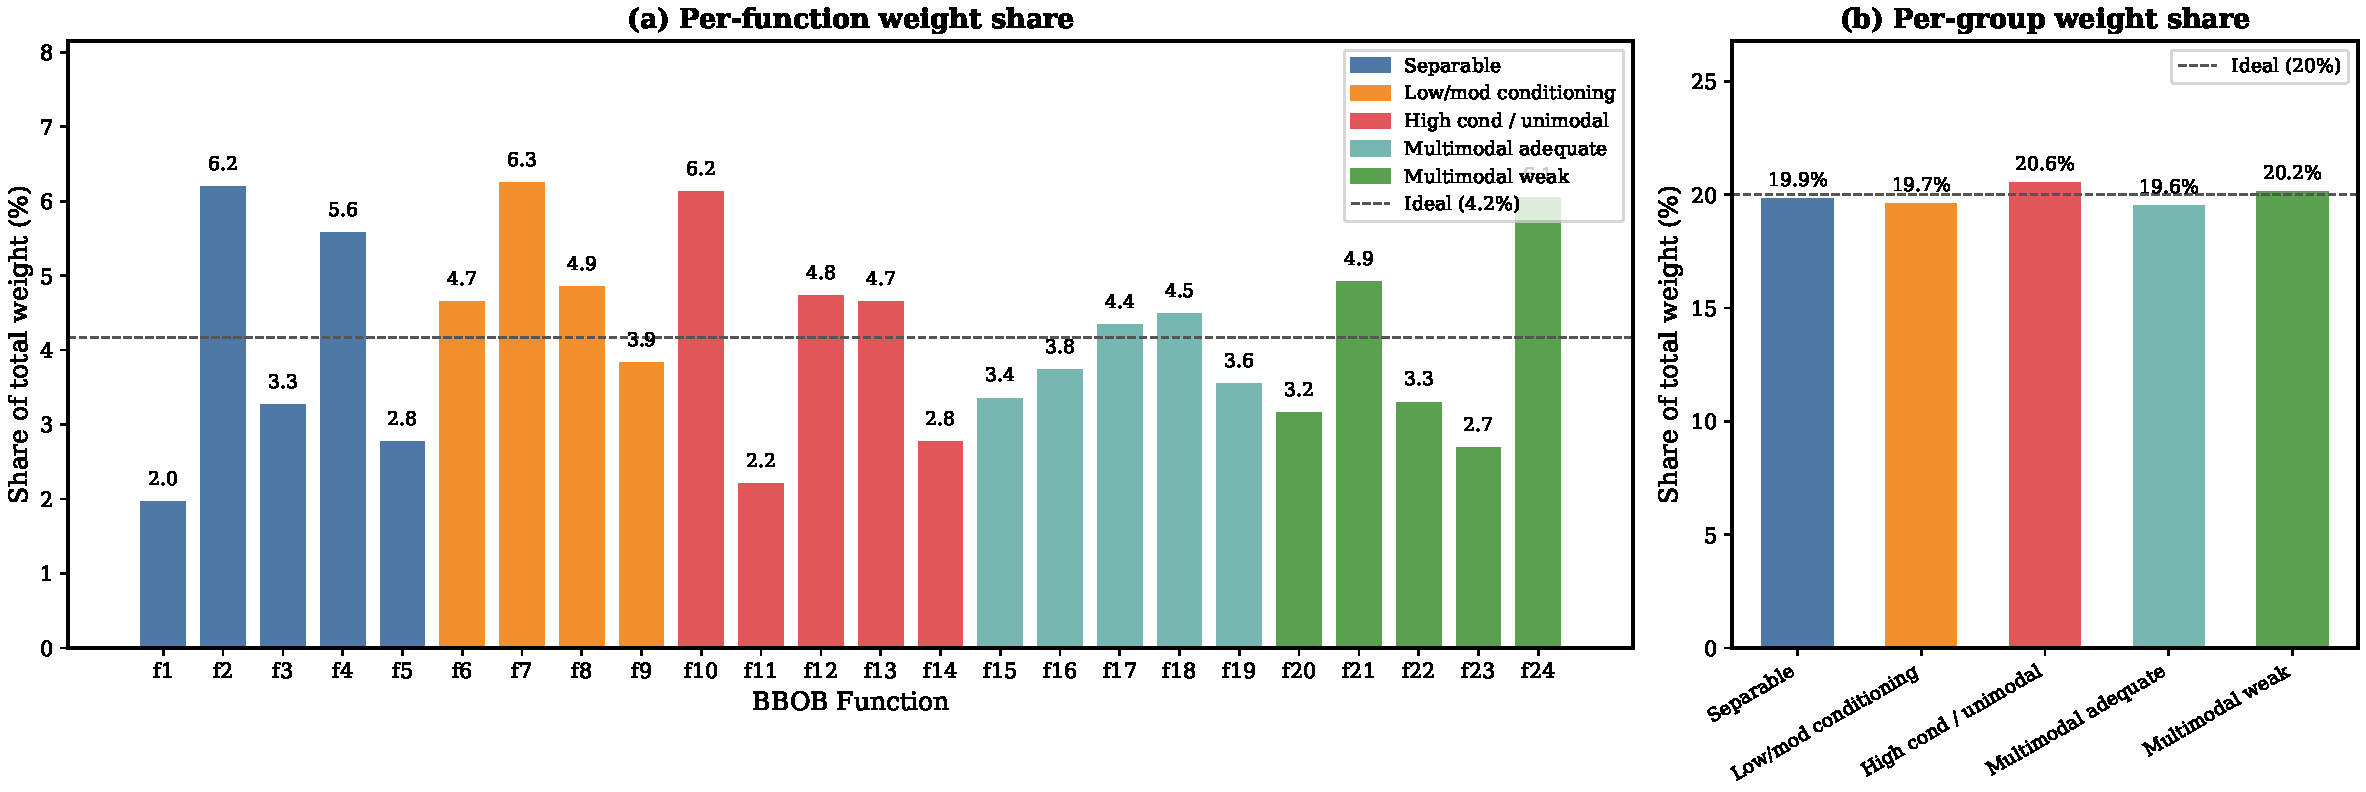
\includegraphics[width=\textwidth]{figures/fig_mabbob_instances.pdf}
  \caption{BBOB function weight distribution of the selected 10 MA-BBOB functions, coloured by BBOB function group. All 24 BBOB functions are covered with near-uniform balance.}
  \label{fig:mabbob-instances}
\end{figure*}

\begin{table*}[!t]
\centering
\caption{BBOB function weights for the 10 selected MA-BBOB functions. Only non-zero contributions are shown (as percentage of total weight). BBOB functions are grouped into separable (f1--f5), low/moderate conditioning (f6--f9), high conditioning/unimodal (f10--f14), multimodal adequate (f15--f19), multimodal weak (f20--f24).}
\label{tab:instance-weights}
\footnotesize
\begin{tabular}{@{}r|ccccc|cccc|ccccc|ccccc|ccccc@{}}
\toprule
& \multicolumn{5}{c|}{\textbf{Sep.}} & \multicolumn{4}{c|}{\textbf{Low/mod}} & \multicolumn{5}{c|}{\textbf{High/uni}} & \multicolumn{5}{c|}{\textbf{MM adeq.}} & \multicolumn{5}{c}{\textbf{MM weak}} \\
\textbf{Func.} & \footnotesize 1 & \footnotesize 2 & \footnotesize 3 & \footnotesize 4 & \footnotesize 5
& \footnotesize 6 & \footnotesize 7 & \footnotesize 8 & \footnotesize 9
& \footnotesize 10 & \footnotesize 11 & \footnotesize 12 & \footnotesize 13 & \footnotesize 14
& \footnotesize 15 & \footnotesize 16 & \footnotesize 17 & \footnotesize 18 & \footnotesize 19
& \footnotesize 20 & \footnotesize 21 & \footnotesize 22 & \footnotesize 23 & \footnotesize 24 \\
\midrule
191 & & & & & & 28 & & & & & & & & & & & & & 25 & 21 & 1 & & 25 & \\
277 & 15 & & 14 & & & & 10 & & & 13 & & & 13 & 6 & & & & 20 & & & & 6 & & 4 \\
300 & & & 19 & & & & 20 & & & & & 18 & & & & & & 12 & & & 29 & & 2 & \\
412 & & 10 & & & 12 & & & 13 & & 14 & & & & & & & 11 & & 11 & & & & & 29 \\
455 & & 13 & & & & & & 17 & & 14 & 14 & & & & & & & 14 & & & & & & 28 \\
635 & & & & 23 & 4 & & 13 & & & & & 9 & & 16 & & 23 & & & & & & 14 & & \\
648 & 5 & & & 9 & & & 20 & & 18 & & & & 18 & & 17 & & & & & 11 & 2 & & & \\
744 & & 17 & & & & 19 & & & & 10 & & & & 7 & 17 & 15 & 15 & & & & & & & \\
760 & & 1 & & 9 & 12 & & & 4 & 20 & & 7 & & 15 & & & & & & & & 17 & 14 & & \\
843 & & 21 & & 14 & & & & 14 & & 10 & 2 & 20 & & & & & 18 & & & & & & & \\
\bottomrule
\end{tabular}
\\[0.3em]
{\scriptsize Values are percentages of total weight. Empty cells indicate zero weight.}
\end{table*}

At each generation the LLM receives a prompt assembled from a role description, a task specification, an example algorithm, a feedback string reporting that algorithm's performance, an optional mutation prompt, and an output-format constraint. The role, task, and output-format portions are taken verbatim from LLaMEA~\cite{vanStein2024LLaMEA}. The full prompt template is shown below.

\begin{lstlisting}[numbers=none,breakautoindent=false,breakindent=0pt,xleftmargin=0pt,basicstyle=\ttfamily\scriptsize]
You are a highly skilled computer scientist in the field of natural computing. Your task is to design novel metaheuristic algorithms to solve black box optimization problems.

The optimization algorithm should handle a wide range of tasks, which is evaluated on the BBOB test suite of 24 noiseless functions. Your task is to write the optimization algorithm in Python code to minimize the function value. The code should contain an `__init__(self, budget, dim)` function and the function `def __call__(self, func)`, which should optimize the black box function `func` using `self.budget` function evaluations.

The func() can only be called as many times as the budget allows, not more. Each of the optimization functions has a search space between -5.0 (lower bound) and 5.0 (upper bound). The dimensionality can be varied.

Give an excellent and novel heuristic algorithm to solve this task.

An example of such code is as follows:
<example algorithm>

Feedback:

The algorithm <algorithm name> got an average Area over the convergence curve (AOCC, 1.0 is the best) score of <score> with standard deviation <std>.

<mutation prompt>

Provide the Python code and a one-line description with the main idea (without enters). Give the response in the format:
# Description: <short-description>
# Code:
```python
<code>
```
\end{lstlisting}

On the first generation the example is \texttt{RandomSearch} (reproduced in \cref{app:randomsearch}) and no mutation prompt is added. From the second generation onwards, the previous best algorithm replaces \texttt{RandomSearch} as the example, and the mutation prompt is drawn from the dual-prompt configuration identified as effective by van Stein et al.~\cite{vanStein2025Behaviour}. With 90\% probability the LLM receives a \emph{refine} prompt (``\textit{Refine and simplify the selected algorithm to improve it}''), and with 10\% probability an \emph{explore} prompt (``\textit{Generate a new algorithm that is different from those tried before}''). This split balances exploitation of promising algorithm structures with exploration of novel designs. The 90/10 ratio is our own choice and to our knowledge no systematic study of its optimality exists.

The offspring then competes against its parent under elitist $(1+1)$ selection. It replaces the parent only if it achieves equal or better fitness, and the surviving algorithm becomes the parent for the next generation. Recent work has explored larger population sizes. Van Stein et al.~\cite{vanStein2025Behaviour} compare six LLaMEA configurations including population-based variants with $\mu/\lambda = 4/12$, and the SAGE experiments~\cite{vanStein2026LLaMEASAGE} use $4$ parents and $16$ offspring. Among the six configurations in the Behaviour Space study~\cite{vanStein2025Behaviour}, the elitist $(1+1)$ variant (LLaMEA-4) outperformed the population-based alternatives, and we retain it for that reason.

After each evaluation, the LLM receives a feedback string reporting the algorithm's performance. Standard (vanilla) feedback reports only the AOCC score and its standard deviation across evaluation runs. Our experiments augment this string with additional behavioural feature information detailed in in \cref{sec:meth-feedback-screening}.

% ---------------------------------------------------------------------------
\section{Benchmark Configuration}
\label{sec:meth-benchmark}

Candidate algorithms are evaluated on MA-BBOB~\cite{vermetten2023mabbob}. Each MA-BBOB function is parameterised by a weight vector over the 24 BBOB functions. All functions used in this thesis are 5-dimensional with search bounds $[-5, 5]^5$.

This thesis uses two function sets drawn from the same 1{,}000-function MA-BBOB pool. The first three stages use a ten-function set, sized to discriminate between models, features, and feedback formats while keeping screening compute tractable across the many models, conditions, and seed replicates that those stages require. Stage~4 uses an extended twenty-function set, disjoint from the screening set, both to give the head-to-head comparison tighter AOCC variance bands and to test that the conclusions of Stages~1--3 generalise to functions the pipeline was not implicitly tuned on.

Both function sets are selected by the greedy forward procedure in \cref{alg:instance-selection}. At each step every remaining function is scored as a potential addition to the current set, with the score favouring candidates that cover BBOB functions not yet represented, that bring the five group shares closer to the ideal 20\% each, and that distribute weight evenly across BBOB functions. Missing BBOB function coverage dominates the score, ensuring all 24 BBOB functions are included before the procedure optimises for balance among individual BBOB function representation. For the ten-function screening set the resulting selection covers all 24 BBOB functions with group shares within $\pm$0.6\% of the ideal 20\% (\cref{fig:mabbob-instances}). \cref{tab:instance-weights} shows the per-function weight breakdown, where each MA-BBOB function blends between 5 and 9 BBOB functions.

\begin{algorithm}[t]
\caption{Greedy MA-BBOB function selection. At each step the candidate whose addition most reduces missing BBOB function count, group imbalance, and per-BBOB-function weight variability is selected.}
\label{alg:instance-selection}
\SetKwInOut{Input}{Input}
\SetKwInOut{Output}{Output}
\Input{$\mathbf{W} \in \mathbb{R}^{1000 \times 24}$ (weight matrix), $k = 10$}
\Output{Selected function set $S$}
$S \gets \varnothing$\;
\For{$i \gets 1$ \KwTo $k$}{
  \ForEach{$c \notin S$}{
    $\mathbf{w} \gets$ column sums of $\mathbf{W}[S \cup \{c\}]$\;
    $m \gets |\{j : w_j = 0\}|$\;
    $\sigma_g \gets \operatorname{std}(\{w_g / \sum w : g \in \text{groups}\})$\;
    $\mathrm{CV} \gets \operatorname{std}(\mathbf{w}_{>0}) / \operatorname{mean}(\mathbf{w}_{>0})$\;
    $\operatorname{score}(c) \gets -100\,m - 10\,\sigma_g - \mathrm{CV}$\;
  }
  $c^* \gets \arg\max_c \;\operatorname{score}(c)$\;
  $S \gets S \cup \{c^*\}$\;
}
\Return{$S$}
\end{algorithm}

The twenty-function Stage~4 set is produced by the same procedure with the ten-function screening set excluded from the candidate pool, ensuring disjointness. The resulting subset covers all 24 BBOB functions with a coefficient of variation of $0.080$ across BBOB function weight totals, and gives the five BBOB function groups shares within $\pm$1.3\% of the ideal 20\%. The BBOB function weight distribution and per-function breakdown are reported in \cref{app:instance-selection-stage4}.

This selection procedure was used to mitigate design bias inherited from the underlying BBOB function set. MA-BBOB is itself a technique for reducing such bias by allowing arbitrary affine combinations of the 24 base functions, but because our function sets are sampled from a finite MA-BBOB pool, residual structure from BBOB persists. The base functions share landscape characteristics within their group as exposed by exploratory landscape analysis~\cite{long2023bbobinstance}, and the five groups are unevenly populated (4 functions in low/moderate conditioning, 5 in each of the others). Selecting for uniform BBOB-function coverage and balanced group shares at the contribution-weight level minimises the influence of any single function or group on aggregated performance, though some residual bias from the fixed BBOB pool is unavoidable.

Each candidate algorithm is evaluated on every function in the active set over 5 configuration instances. For Stages~1--3 this yields 50 independent runs per candidate (10 functions $\times$ 5 instances) and for Stage~4 it yields 100 (20 functions $\times$ 5 instances). The evaluation budget per run is $T = 2{,}000 \times d = 10{,}000$ function evaluations (FEs), following the BBOB convention~\cite{hansen2021coco}.

Algorithm quality is measured by the Area Over the Convergence Curve (AOCC). For a single run of algorithm $a$ on function $f$ and instance $s$, with evaluation budget $T$, the normalised per-run area is:
\begin{equation}
\label{eq:per-run-area}
A(\mathbf{y}_{a,f,s}) = \frac{1}{T} \sum_{t=1}^{T} \left(1 - \frac{\min(\max(y_t, lb), ub) - lb}{ub - lb}\right)
\end{equation}
where $\mathbf{y}_{a,f,s} = (y_1, \ldots, y_T)$ is the sequence of log-scaled best-so-far fitness values, and $ub = 10^{2}$, $lb = 10^{-8}$ are the clipping bounds. The AOCC for a candidate algorithm is the mean of $A$ over all functions $f$ and instances $s$:
\begin{equation}
\label{eq:aocc}
\text{AOCC}(a) = \frac{1}{N} \sum_{f=1}^{F} \sum_{s=1}^{S} A(\mathbf{y}_{a,f,s})
\end{equation}
In Stages~1--3 we have $F = 10$ and $S = 5$, giving $N = 50$ independent runs per candidate. Stage~4 uses $F = 20$, raising $N$ to 100. This single scalar is reported to the LLM as feedback.

For every successful candidate evaluation, the full trajectory ($T = 10{,}000$ evaluations of decision variables and fitness values) is logged via IOHexperimenter, and all 32 behavioural features described in \cref{ch:features} are computed post-hoc. Features are averaged across the 50 runs per candidate to produce a single feature vector per algorithm. This dataset, comprising feature vectors for every valid candidate across all models and seeds, forms the basis for the Stage~2 feature analysis.

% ---------------------------------------------------------------------------
\section{LLM Screening}
\label{sec:meth-screening}

Stage~1 screens LLMs for their ability to reliably generate high-quality metaheuristics for continuous black-box optimisation. Small language models vary substantially in their ability to generate valid optimisation code, and inference cost matters when each evolutionary run requires hundreds of LLM calls. The screening identifies the model that is later carried forward into Stages~3 and~4, and supplies the dataset of trajectories on which Stage~2 is built.

Ten models are evaluated, spanning locally served open-weight models and cloud API models. \cref{tab:models} lists all models with their parameter counts and providers. Each model runs the LLaMEA loop for 100 candidates across 5 independent seeds, all using vanilla AOCC-only feedback, for a total of $10 \text{ models} \times 5 \text{ seeds} \times 100 \text{ candidates} = 5{,}000$ LLaMEA iterations. All 32 behavioural features are computed for every successful candidate, producing a dataset of several thousand algorithm--feature observations.

\begin{table}[t]
\centering
\caption{LLMs evaluated in Stage~1. Local models are served via Ollama~\cite{ollama} or vLLM~\cite{kwon2023vllm}. API models use Google's Gemini API. Parameter counts reflect total (not active) parameters.}
\label{tab:models}
\footnotesize
\begin{tabular}{@{}llrl@{}}
\toprule
\textbf{Model} & \textbf{Provider} & \textbf{Params} & \textbf{Backend} \\
\midrule
Qwen3.5 4B   & Qwen/Alibaba~\cite{qwen3}          & 4B  & Ollama \\
Qwen3.5 9B   & Qwen/Alibaba~\cite{qwen3}          & 9B  & vLLM \\
Qwen3.5 27B  & Qwen/Alibaba~\cite{qwen3}          & 27B & Ollama \\
RNJ-1 8B     & Essential AI~\cite{rnj1}            & 8B  & Ollama \\
Devstral Small~2 & Mistral AI~\cite{devstral2}     & 24B & Ollama \\
OLMo~3 7B    & Allen AI~\cite{olmo3}               & 7B  & Ollama \\
OLMo~3 32B Think & Allen AI~\cite{olmo3}           & 32B & Ollama \\
Granite~4 Micro  & IBM~\cite{granite4}             & 3B  & vLLM \\
\midrule
Gemini~3 Pro     & Google~\cite{gemini3pro}      & --- & API \\
Gemini~3 Flash   & Google~\cite{gemini3flash}      & --- & API \\
\bottomrule
\end{tabular}
\end{table}

Models are compared on three factors. The failure rate is the fraction of candidates that fail to produce valid fitness, due to syntax errors, interface mismatches, or runtime exceptions. The best AOCC is the highest AOCC achieved across all 5 seeds, measuring peak algorithm quality. The inference efficiency is the rate of tokens generated per second, which determines wall-clock time per evolutionary run. The model that performs best across these factors is carried forward into later stages.

% ---------------------------------------------------------------------------
\section{Feature Analysis and Selection}
\label{sec:meth-feature-selection}

Stage~2 analyses the Stage~1 dataset of behavioural feature vectors for all valid candidates across 10 models and 5 seeds to determine which of the 32 features in \cref{ch:features} are most predictive of algorithm quality, and to select a tractable subset for the feedback experiments. The target subset size is fixed at ten features. The cap is set by the available compute budget and API costs rather than statistical considerations. Stage~3 evaluates each retained feature in three framings across 5 seeds of 100 candidates with the model identified in Stage~1, and the per-feature cost of running these evaluations makes a larger subset infeasible. Selecting on predictive power keeps the ten most informative features in the loop, while pruning redundancy ensures they capture distinct aspects of behaviour rather than re-stating the same signal.

Three complementary approaches are applied to rank the 32 features, each capturing a different aspect of feature quality. Spearman rank correlation~\cite{spearman1904proof} captures monotonic associations between each feature and AOCC across all valid candidates, regardless of functional form. Random Forest permutation importance~\cite{breiman2001randomforests} captures non-linear and interaction effects. A regression model is trained to predict AOCC from all 32 features, and each feature's importance is measured by the decrease in out-of-bag $R^2$ when its values are permuted. Kolmogorov--Smirnov distributional effect size~\cite{kolmogorov1933} captures distributional separation between high- and low-quality algorithms. It computes the KS statistic between feature distributions of the top-25\% and bottom-25\% candidates by AOCC, after winsorising each feature at the 1st and 99th percentiles to limit the influence of outliers.

Each method produces a ranked list of 32 features. The three rankings are aggregated via Borda count~\cite{black1958theory}. Each feature receives $32 - r_i$ points from each method (where $r_i$ is its rank in method $i$). Summed scores determine the consensus ranking, with lower values indicating a more informative feature.

The consensus list is then de-duplicated by greedy redundancy pruning. Features are processed in Borda-rank order. If a candidate feature has Spearman $|\rho| > \tau$ with any already-selected feature, it is discarded as redundant. To determine $\tau$ we sweep across the range $[0.5, 1.0]$ in steps of $0.05$ and record, at each value, the surviving subset and its mean Borda rank, then pick the value that produces the largest single-step improvement in mean Borda rank. This corresponds to the elbow in the quality-vs-threshold curve, beyond which further tightening prunes already-distinct features without comparable gain. The top ten survivors of pruning at this threshold form the final feature subset taken into Stage~3.

% ---------------------------------------------------------------------------
\section{Feedback Format Screening}
\label{sec:meth-feedback-screening}

Stage~3 tests whether the framing of behavioural feedback affects the performance of LLM-generated algorithms. Each feature selected in Stage~2 is embedded into the feedback string under three contrasting framings (neutral, directional, comparative), with one feature added at a time so that effects can be attributed to the framing rather than to the joint presence of multiple features. The comparative format is excluded for \texttt{longest\_no\_improvement\_streak} because that feature has a U-shaped relationship with AOCC for which a single reference target would be misleading, leaving 29 active conditions.

The neutral format reports the feature value and its definition, without any indication of whether high or low values are desirable,

\begin{quote}
\small\itshape
The algorithm X got an average AOCC score of 0.7234 with standard deviation 0.0891. It achieved a \texttt{step\_size\_autocorrelation} of 0.8421 with standard deviation 0.0532, which measures whether large steps tend to follow large steps, capturing momentum in the search.
\end{quote}

The directional format extends the neutral format with a sentence indicating which direction is associated with better performance. The direction is derived from the prior Spearman correlation analysis,

\begin{quote}
\small\itshape
\ldots capturing momentum in the search. Higher values are associated with better performance, indicating consistent, smooth step-size adaptation rather than erratic jumps.
\end{quote}

The comparative format replaces the directional guidance with a distance-aware comparison against a concrete reference value. The reference is the median feature value of top-10\% algorithms by AOCC from the LLM screening stage. The normalised distance from this reference is $d = (v_{\text{ref}} - v) / (v_{\text{ref}} - v_{\text{bot25}})$, where $v$ is the candidate's feature value, $v_{\text{ref}}$ is the top-10\% median, and $v_{\text{bot25}}$ is the bottom-25\% median. This denominator provides a meaningful scale representing the range between good and bad algorithms for each feature. The numeric reference value is reported in every tier so that the LLM has a concrete target rather than only a qualitative direction. The wording of the comparison itself adapts across four tiers, strengthening progressively as $d$ grows:

\begin{enumerate}
  \item \textbf{Already meets reference} ($d \leq 0$): ``\textit{This already meets or exceeds the top-performing reference of 0.9070. Maintain this.}''
  \item \textbf{Close to reference} ($0 < d \leq 0.15$): ``\textit{This is close to the top-performing reference of 0.9070. A small increase could help.}''
  \item \textbf{Moderate gap} ($0.15 < d \leq 0.50$): ``\textit{This is moderately below the top-performing reference of 0.9070. Consider increasing this value.}''
  \item \textbf{Far from reference} ($d > 0.50$): ``\textit{This is far from the reference of 0.9070. Increasing this value is a priority.}''
\end{enumerate}

Each condition runs for 100 candidates across 5 independent seeds, for a total of $29 \text{ conditions} \times 5 \text{ seeds} \times 100 \text{ candidates} = 14{,}500$ LLaMEA iterations, and the vanilla AOCC-only results from Stage~1 serve as the baseline for measuring performance improvements.

% ---------------------------------------------------------------------------
\section{Full-Benchmark Comparison}
\label{sec:meth-stage4}

\begin{figure*}[!t]
  \centering
  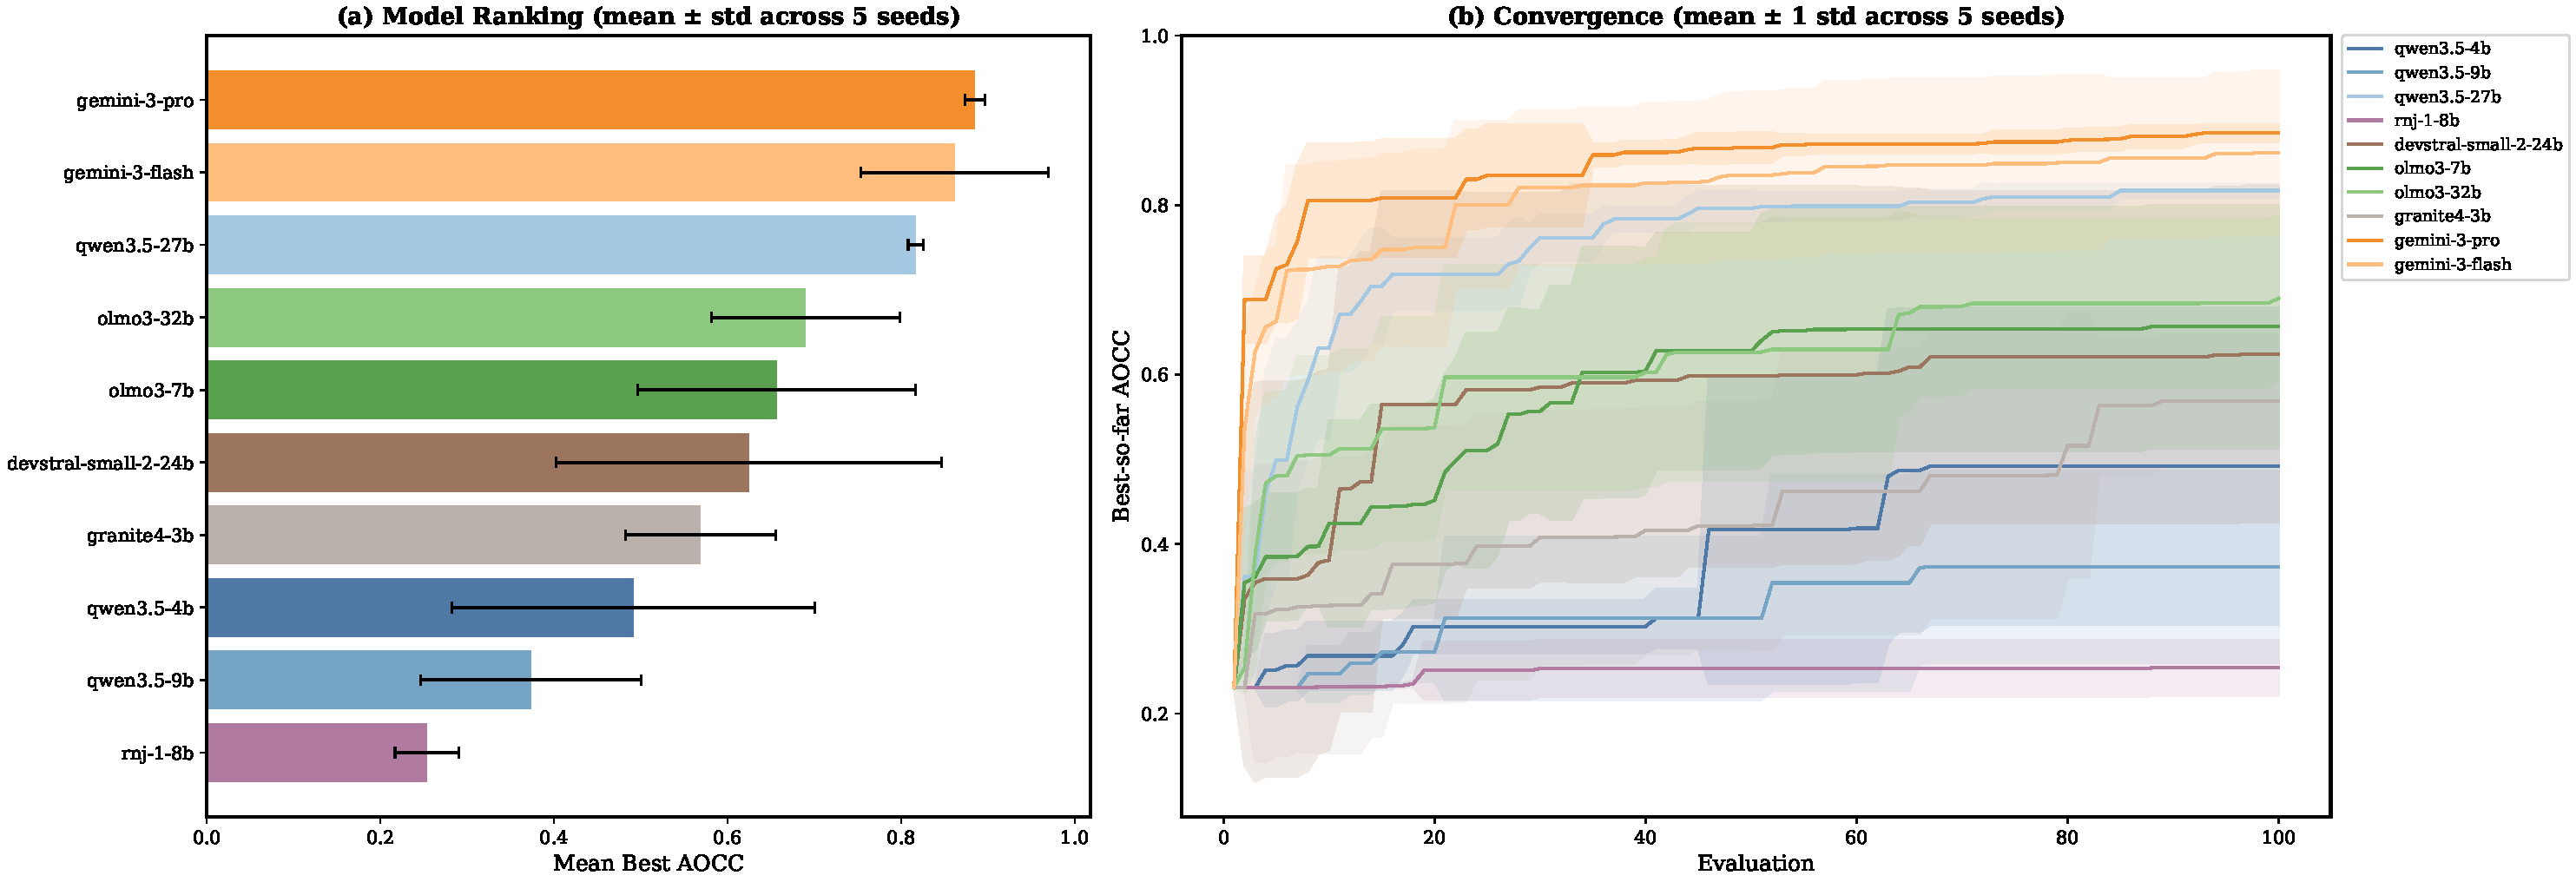
\includegraphics[width=\textwidth]{figures/fig_model_screening.pdf}
  \caption{LLM screening results. (a)~Mean best AOCC by model ($\pm$ std across 5 seeds). (b)~Best-so-far AOCC over 100 evaluations, averaged across 5 seeds. Shaded regions show $\pm$1 std.}
  \label{fig:model-screening}
\end{figure*}

\begin{table}[t]
\centering
\caption{Stage~1 model ranking (100 candidates $\times$ 5 seeds, vanilla feedback). Fail\% and AOCC averaged across seeds ($\pm$ std).}
\label{tab:model-ranking}
\footnotesize
\begin{tabular}{@{}rlrrr@{}}
\toprule
\textbf{\#} & \textbf{Model} & \textbf{Fail\%} & \textbf{AOCC} & \textbf{h/run} \\
\midrule
1  & Gem.~3 Pro    & 10.2  & .885$\pm$.011 & 5.1 \\
2  & Gem.~3 Flash  & \textbf{2.0} & .862$\pm$.108 & 3.9 \\
3  & Qwen3.5 27B   & 41.0  & .817$\pm$.009 & 38.9 \\
4  & OLMo~3 32B    & 13.2  & .690$\pm$.109 & 39.3 \\
5  & OLMo~3 7B     & 27.6  & .657$\pm$.160 & 18.4 \\
6  & Devstral~2    & 32.6  & .625$\pm$.222 & 5.0 \\
7  & Granite~4 3B  & 53.8  & .569$\pm$.087 & \textbf{0.6} \\
8  & Qwen3.5 4B    & 76.2  & .492$\pm$.209 & 7.9 \\
9  & Qwen3.5 9B    & 91.6  & .373$\pm$.127 & 3.0 \\
10 & RNJ-1 8B      & 34.6  & .254$\pm$.037 & 14.5 \\
\bottomrule
\end{tabular}
\end{table}

Stage~4 is a head-to-head comparison of four feedback conditions, run on the twenty-function MA-BBOB set with longer evolutionary runs and more independent seeds than the screening stages so condition differences can be detected at the resolution required to draw substantive conclusions.

The vanilla condition uses AOCC-only feedback, identical to the baseline used in Stage~1, repeated here on the new function set as the reference point against which all other conditions are measured. The neutral condition extends AOCC with trajectory-derived behavioural features, isolating the contribution of distal (behavioural) feedback. The sage condition pairs AOCC with structural code-level guidance from LLaMEA-SAGE~\cite{vanStein2026LLaMEASAGE}, used unmodified, isolating the contribution of proximal (structural) feedback. The combined condition appends both behavioural and structural feedback in the same prompt, testing whether the two channels are complementary or redundant.

The behavioural feedback uses the five features ranked highest by mean best AOCC across the Stage~3 neutral conditions. These features are \texttt{intensification\_ratio}, \texttt{dimension\_convergence\_heterogeneity}, \texttt{fitness\_plateau\_fraction}, \texttt{avg\_improvement}, and \texttt{improvement\_spatial\_correlation}. All five are appended to the AOCC feedback string in the neutral framing. The five-feature cap keeps the prompt compact while still spanning the four functional categories of \cref{ch:features} (intensification, convergence, stagnation, and exploration).

Benchmark parameters from \cref{sec:meth-benchmark} are inherited unchanged, with the Stage~4 function set detailed in \cref{app:instance-selection-stage4}. Each condition runs for 500 candidates per seed, five times the screening budget, giving feedback signals that act gradually a fair chance to express their effect. Ten independent seeds per condition (double the previous stages) tighten the variance bands when comparing condition means and make condition-vs-condition differences detectable at smaller effect sizes. The total compute is $4 \text{ conditions} \times 10 \text{ seeds} \times 500 \text{ candidates} = 20{,}000$ candidate algorithms, each evaluated over $20 \text{ functions} \times 5 \text{ instances} = 100$ MA-BBOB runs hence totalling 2,000,000 MA-BBOB function evaluations.

Finally, to assess how the strongest generated algorithms generalise beyond the twenty-function set and the 5-dimensional regime in which they were developed, the best-found algorithm from each of the conditions is re-evaluated on the full $1{,}000$-instance MA-BBOB pool. A generic CMA-ES~\cite{hansen2001cmaes} and \texttt{NeighborhoodAdaptiveDE} (NADE)~\cite{vanStein2025NeighborhoodDE}, the winner of the 2025 MA-BBOB competition, are used as basline performance references. Each of the six algorithms runs on all $1{,}000$ MA-BBOB functions across 5 instance seeds and three dimensionalities $d \in \{5, 10, 20\}$, under a $2{,}000d$ FE budget per run, totalling approximately $2.1 \times 10^9$ function evaluations.

% ---------------------------------------------------------------------------
\section{Infrastructure}
\label{sec:meth-infrastructure}

All experiments are executed on the LIACS SLURM cluster node \textbf{saronite}, equipped with 4$\times$ NVIDIA L40S GPUs (48\,GB each), 2$\times$ 32-core Intel Xeon Gold 6438M CPUs, and 512\,GB RAM. Most local models are served via Ollama~\cite{ollama}, which processes requests sequentially in a queue. For Qwen3.5~9B and Granite~4~Micro, we use vLLM~\cite{kwon2023vllm}, which supports continuous batching and manages KV caches efficiently via PagedAttention~\cite{kwon2023vllm}. This allows multiple seeds to issue concurrent inference requests rather than waiting in a serial queue, reducing wall-clock time per evolutionary run. Gemini~3 models~\cite{gemini3pro, gemini3flash} are accessed through Google's Gemini API. All code, configuration, and analysis notebooks are available in the thesis repository.\footnote{\url{https://github.com/maxharell/thesis}} The BLADE~\cite{vanStein2025BLADE} and LLaMEA~\cite{vanStein2024LLaMEA} repositories are included as Git submodules, with minor modifications to support custom feedback strings and extended behavioural metric logging.

% !TEX root = ../thesis.tex
% =============================================================================
% Section 5: Results
% =============================================================================

\chapter{Results}
\label{ch:results}

\begin{figure*}[!t]
  \centering
  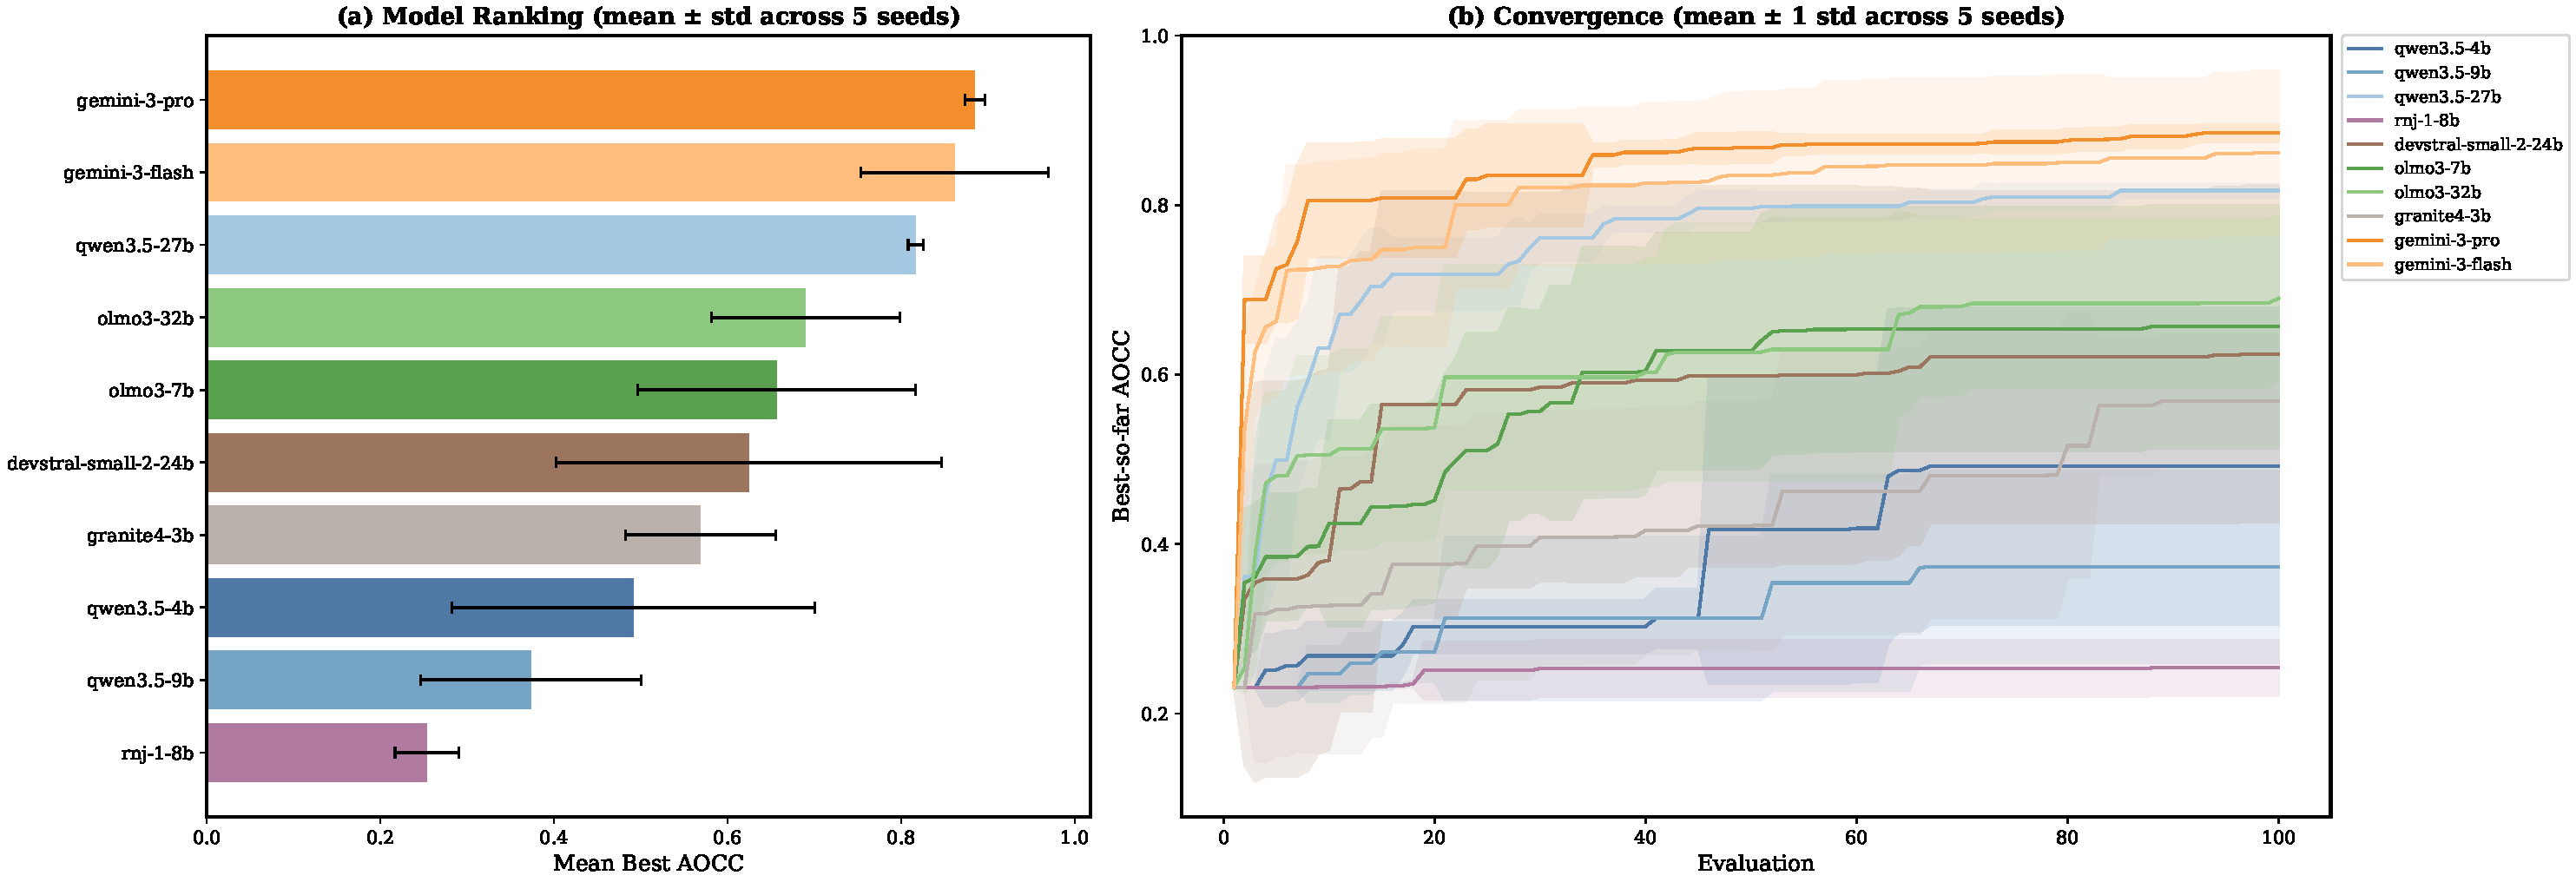
\includegraphics[width=\textwidth]{figures/fig_model_screening.pdf}
  \caption{LLM screening results. (a)~Mean best AOCC by model ($\pm$ std across 5 seeds). (b)~Best-so-far AOCC over 100 evaluations, averaged across 5 seeds. Shaded regions show $\pm$1 std.}
  \label{fig:model-screening}
\end{figure*}

This chapter reports the experimental outcomes of the four-stage pipeline described in \cref{ch:methodology}. \Cref{sec:results-screening} ranks the ten candidate LLMs and identifies the model carried into later stages. \Cref{sec:results-features} reduces the 32 behavioural features to a tractable, predictive subset. \Cref{sec:results-feedback} compares the three feedback framings of those features against the vanilla baseline. \Cref{sec:results-stage4} runs the head-to-head comparison of vanilla, neutral-behavioural, SAGE, and combined feedback on the twenty-function MA-BBOB set with longer evolutionary runs and more independent seeds.

% ===========================================================================
\section{LLM Screening}
\label{sec:results-screening}

\Cref{tab:model-ranking} presents the performance ranking of all 10 models, sorted by mean best AOCC across 5 seeds. The API models clearly dominate. Gemini~3 Pro achieves the highest mean best AOCC of $0.885 \pm 0.011$ with high consistency across seeds, while Gemini~3 Flash follows closely at $0.862$ with the lowest failure rate of any model at just $2.0\%$. The convergence curves in \cref{fig:model-screening}b show that Gemini models improve steadily throughout the full 100-evaluation budget, whereas most open-weight models plateau early or stagnate after initial gains.

\begin{table}[t]
\centering
\caption{Stage~1 model ranking (100 candidates $\times$ 5 seeds, vanilla feedback). Fail\% and AOCC averaged across seeds ($\pm$ std).}
\label{tab:model-ranking}
\footnotesize
\begin{tabular}{@{}rlrrr@{}}
\toprule
\textbf{\#} & \textbf{Model} & \textbf{Fail\%} & \textbf{AOCC} & \textbf{h/run} \\
\midrule
1  & Gem.~3 Pro    & 10.2  & .885$\pm$.011 & 5.1 \\
2  & Gem.~3 Flash  & \textbf{2.0} & .862$\pm$.108 & 3.9 \\
3  & Qwen3.5 27B   & 41.0  & .817$\pm$.009 & 38.9 \\
4  & OLMo~3 32B    & 13.2  & .690$\pm$.109 & 39.3 \\
5  & OLMo~3 7B     & 27.6  & .657$\pm$.160 & 18.4 \\
6  & Devstral~2    & 32.6  & .625$\pm$.222 & 5.0 \\
7  & Granite~4 3B  & 53.8  & .569$\pm$.087 & \textbf{0.6} \\
8  & Qwen3.5 4B    & 76.2  & .492$\pm$.209 & 7.9 \\
9  & Qwen3.5 9B    & 91.6  & .373$\pm$.127 & 3.0 \\
10 & RNJ-1 8B      & 34.6  & .254$\pm$.037 & 14.5 \\
\bottomrule
\end{tabular}
\end{table}


Among open-weight models, performance does not scale with parameter count. Qwen3.5~27B achieves $0.817$, outperforming the larger OLMo~3 32B at $0.690$. Granite~4, the smallest model at just 3B parameters, reaches $0.569$ and outperforms both Qwen3.5~9B at $0.373$ and RNJ-1~8B at $0.254$. This suggests that code generation ability for optimisation algorithms depends more on training data and architecture than on raw scale. Failure rates vary dramatically, from $2.0\%$ for Gemini~3 Flash to $91.6\%$ for Qwen3.5~9B, which fails to produce a valid algorithm class in the vast majority of attempts. Wall-clock time also varies substantially. The two models served via vLLM, Granite~4 at 0.6\,h/run and Qwen3.5~9B at 3.0\,h/run, benefit from continuous batching that allows concurrent seed evaluation. The largest open-weight models, Qwen3.5~27B and OLMo~3 32B, require approximately 39 hours per run under Ollama due to both model size and serial request queuing.

\subsection{Failure Mode Analysis}
\label{sec:results-failures}

Across all 10 models and 5 seeds, 5{,}000 candidates were generated in total, of which $3{,}071$ or $61.4\%$ produced valid fitness scores. The nature of failures differs systematically between strong and weak models. The top performing Gemini models have the lowest failure rates and predominantly fail due to runtime errors, where the generated code has the correct class interface but contains logic bugs that cause exceptions during evaluation. Weaker models instead produce structural failures, generating standalone functions rather than the required Python class or omitting mandatory constructor parameters.


\begin{figure}[t]
  \centering
  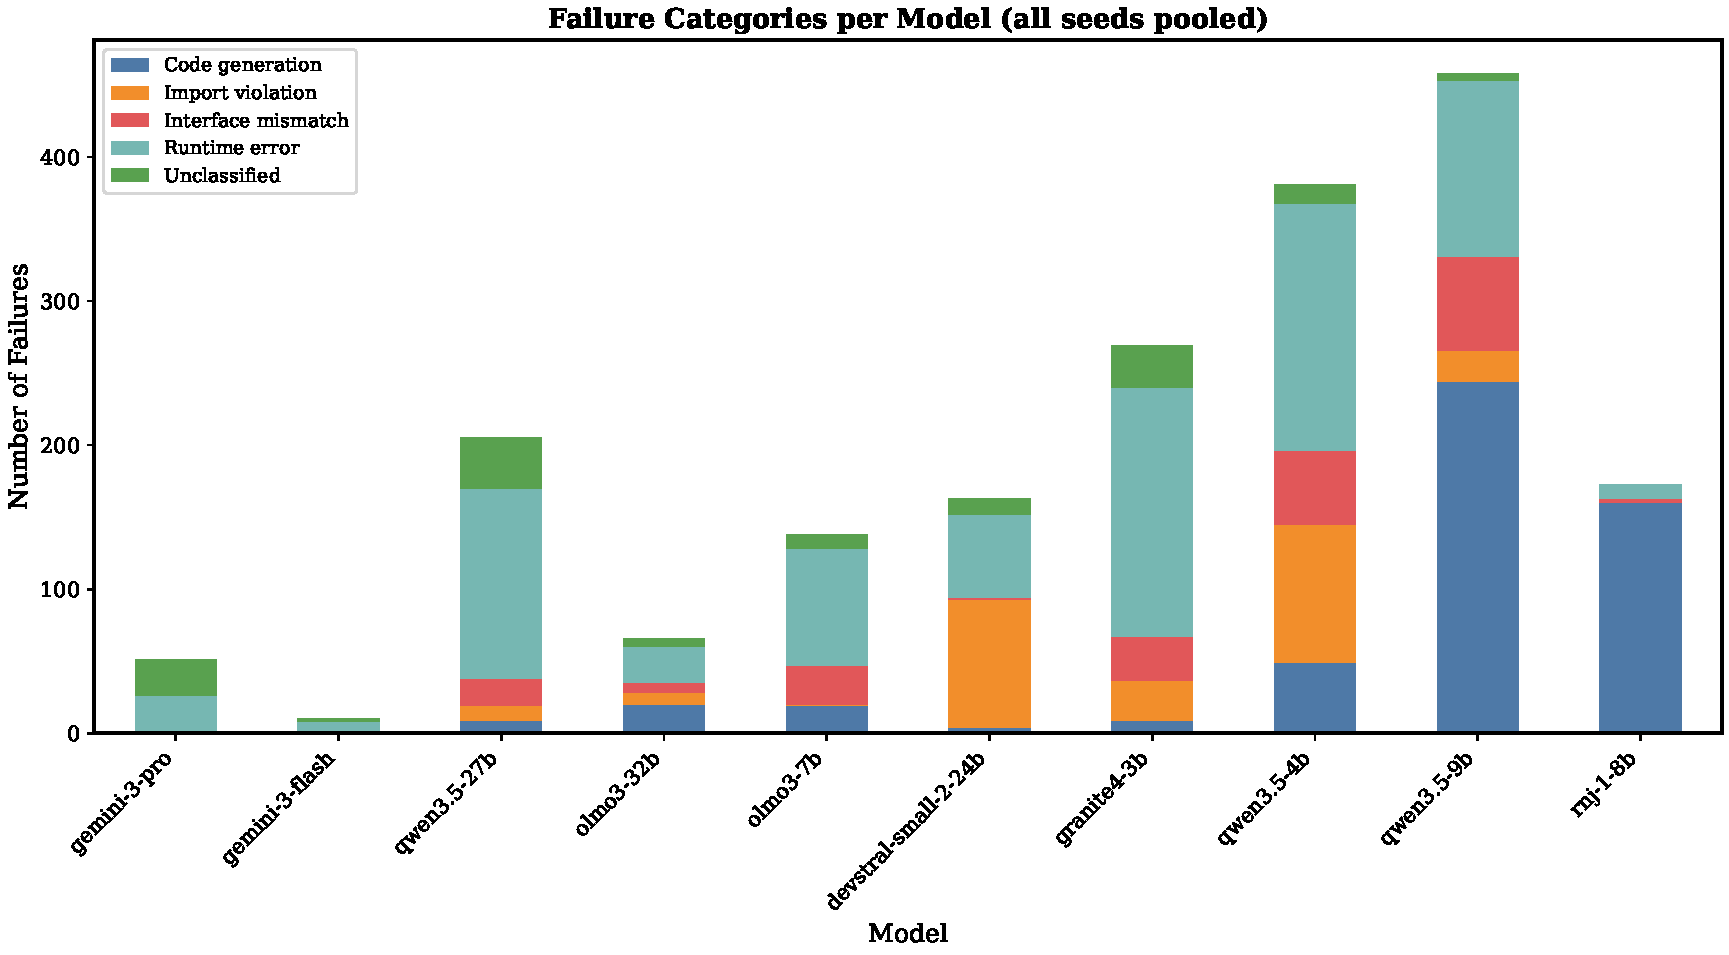
\includegraphics[width=\columnwidth]{figures/fig_failure_modes.pdf}
  \caption{Failure mode distribution by model. Categories include runtime errors (correct interface, logic bugs), structural failures (no class produced), and import errors.}
  \label{fig:failure-modes}
\end{figure}

\subsection{Behavioural Space}
\label{sec:results-behavioural-space}

\begin{figure*}[t]
  \centering
  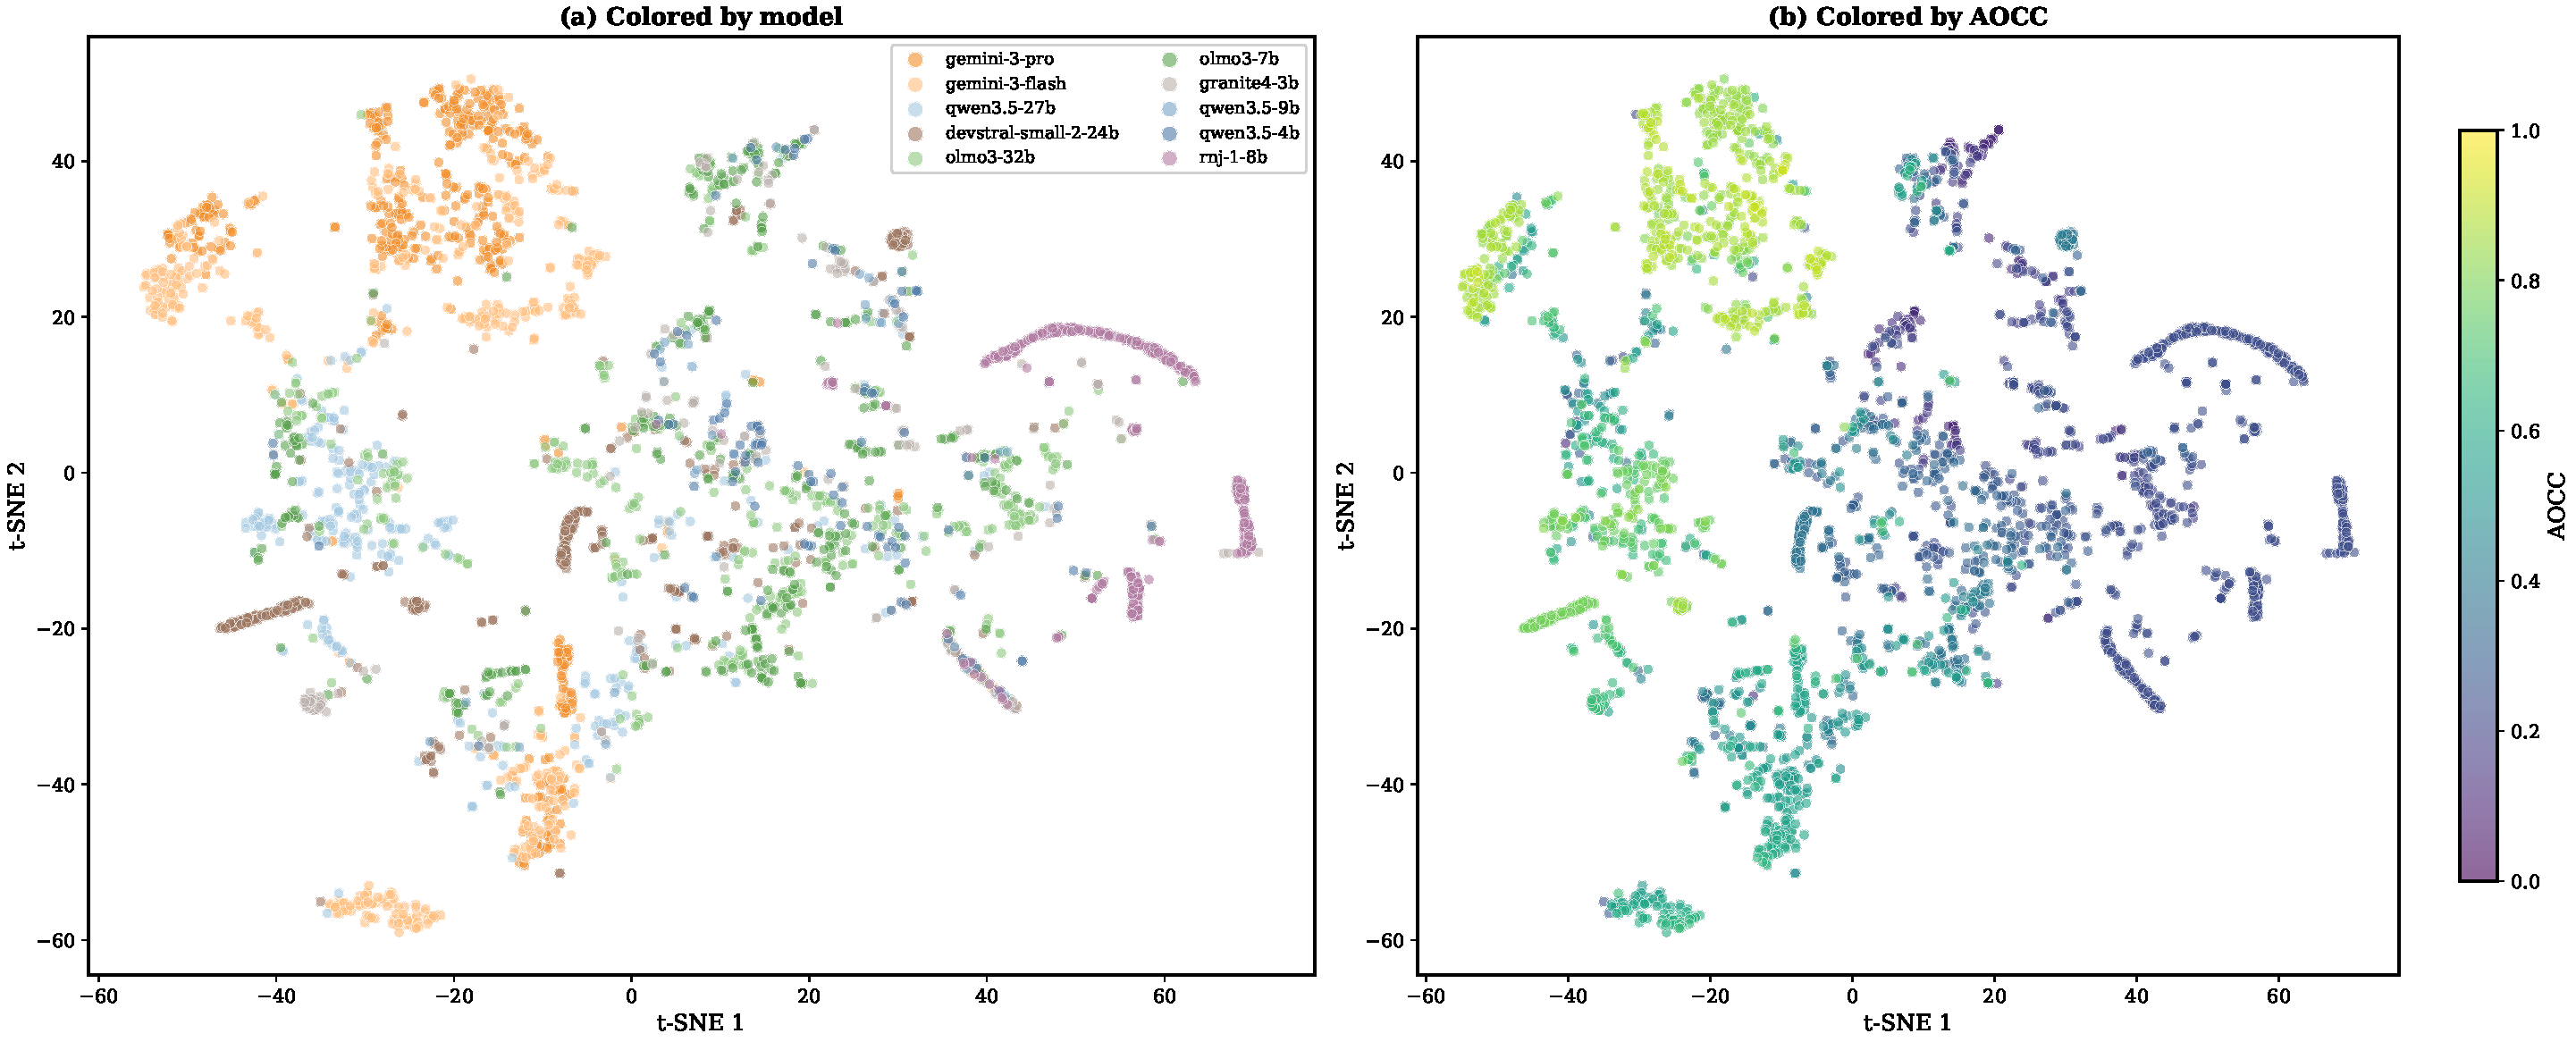
\includegraphics[width=\textwidth]{figures/fig_tsne_behavioral.pdf}
  \caption{t-SNE projection of the behavioural feature space for all $3{,}071$ valid algorithms. (a)~Points coloured by model reveal distinct clustering. Each LLM occupies a characteristic region, with some models forming elongated trajectories indicating incremental refinement. (b)~Points coloured by AOCC show that high-performing algorithms (yellow) concentrate in specific regions, while low-performing ones (purple) spread diffusely.}
  \label{fig:tsne-behavioral}
\end{figure*}

\begin{figure}[p]
  \centering
  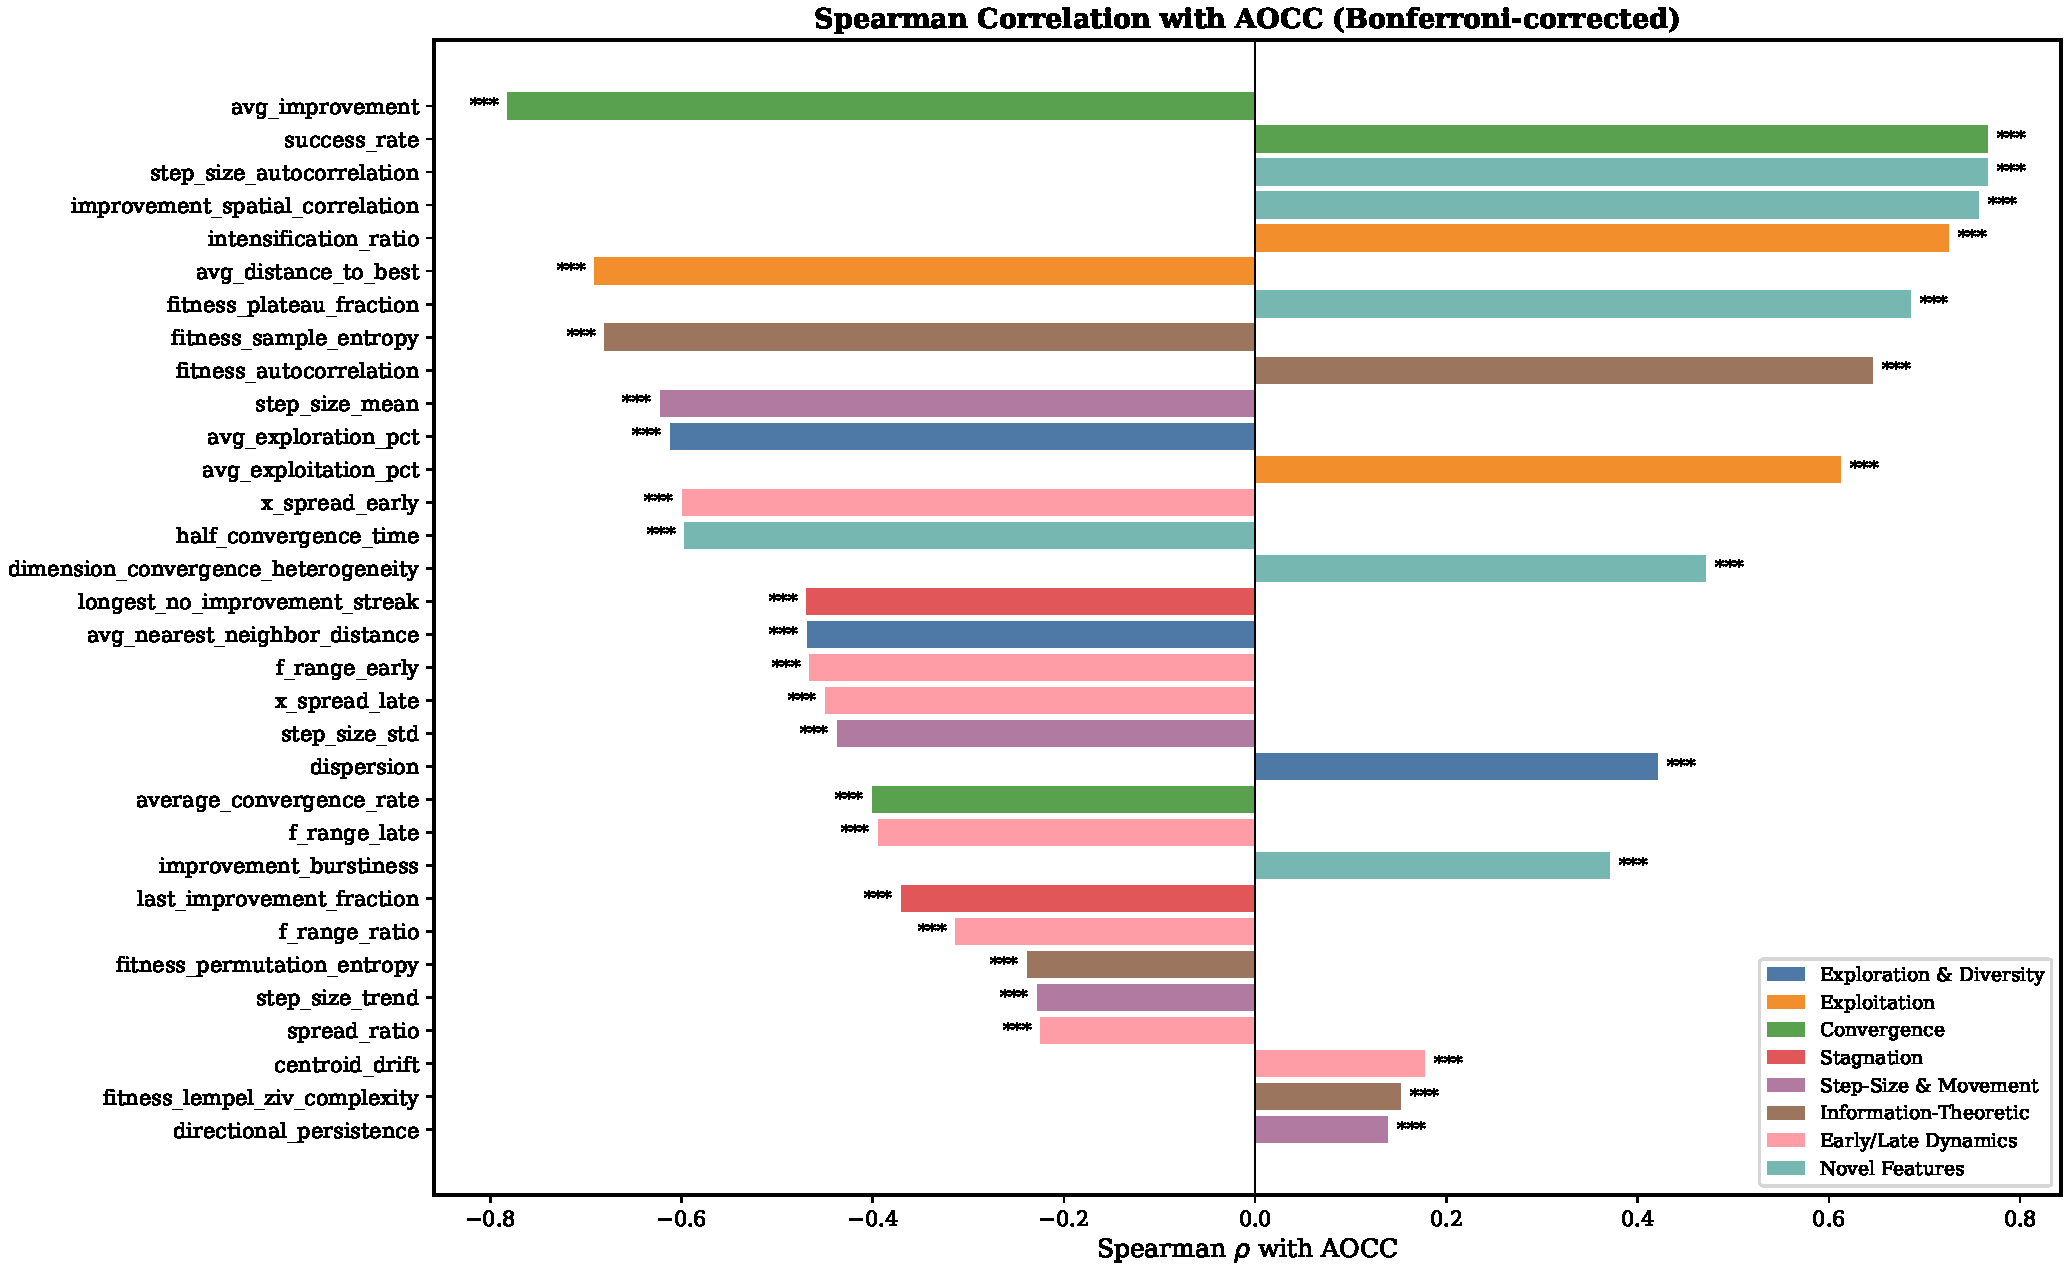
\includegraphics[width=\columnwidth]{figures/fig_spearman.pdf}
  \caption{Spearman rank correlation $\rho$ between each behavioural feature and AOCC across all $3{,}071$ valid candidates, sorted by $|\rho|$ and coloured by feature category. All features significant at $p < 0.001$ after Bonferroni correction.}
  \label{fig:spearman}
\end{figure}

\Cref{fig:tsne-behavioral} projects all valid candidates into a two-dimensional behavioural space via t-SNE on the 32 standardised features. Several patterns emerge. First, algorithms from the same model cluster together, confirming that each LLM produces a characteristic behavioural signature. The Gemini models dominate the upper-left quadrant, which panel~(b) reveals as the high-AOCC region (predominantly yellow-green). Second, several models produce elongated, chain-like trajectories rather than round clusters. RNJ-1 (right side) shows this most clearly, forming distinct arcs that trace the $(1+1)$-ES refinement path through behavioural space. Third, some models fragment into multiple sub-clusters, corresponding to different seeds exploring distinct algorithmic strategies. Fourth, the highest-performing algorithms from open-weight models (Qwen3.5~27B, OLMo~32B) partially overlap with the Gemini cluster, suggesting that strong optimisation behaviour converges to similar behavioural profiles regardless of the generating model. Weaker models (RNJ-1, Qwen3.5~4B) are confined to peripheral, low-AOCC regions with no overlap.

\subsection{Model Selection}
\label{sec:results-model-selection}

Gemini~3 Flash is selected for future experiments based on its combination of competitive AOCC ($0.862$), lowest failure rate ($2.0\%$), and fast inference (3.9h/run). Its vanilla performance across 5 seeds ($0.862 \pm 0.097$) serves as the baseline for all Stage~3 comparisons.

% ===========================================================================

\section{Feature Analysis and Selection}
\label{sec:results-features}

The Stage~1 dataset contains $3{,}071$ valid candidates. Each is accompanied by a 32-dimensional behavioural feature vector computed from its evaluation trajectory. This section determines which features are most predictive of algorithm quality and selects a tractable subset for the feedback experiments.

\subsection{Feature--AOCC Correlations}
\label{sec:results-correlations}

\Cref{fig:spearman} shows the Spearman rank correlation between each of the 32 behavioural features and AOCC. Given the sample size, all 32 correlations are statistically significant at $p < 0.001$ after Bonferroni correction, so significance is not a useful discriminator. Instead, we focus on the magnitude and direction of $\rho$ to understand which behaviours characterise high-performing algorithms.

The five strongest associations are \texttt{avg\_improvement} ($-0.782$), \texttt{success\_rate} ($+0.766$), \texttt{step\_size\_autocorrelation} ($+0.766$), \texttt{improvement\_spatial\_correlation} ($+0.757$), and \texttt{intensification\_ratio} ($+0.725$). Three of these five are introduced to LLaMEA-generated metaheuristic analysis in this thesis.

Examining correlations by feature category reveals a clear behavioural profile of successful algorithms. The \emph{exploitation} features show the strongest positive associations. High \texttt{intensification\_ratio} ($+0.725$) and low \texttt{avg\_distance\_to\_best} ($-0.691$) indicate that good algorithms focus their search near the best-known solution. The \emph{convergence} features reinforce this picture. Low \texttt{avg\_improvement} ($-0.782$) means the algorithm has already found good solutions early, leaving less room for further gains, while high \texttt{fitness\_plateau\_fraction} ($+0.685$) reflects spending more of the budget in a converged state. Among the \emph{step-size and movement} features, \texttt{step\_size\_autocorrelation} ($+0.766$) stands out, indicating that smooth, momentum-driven step sizes outperform erratic adjustments. The \emph{early/late dynamics} features confirm that successful algorithms do not waste early evaluations on broad exploration. \texttt{x\_spread\_early} ($-0.599$) shows that narrower initial search correlates with higher AOCC. In contrast, the \emph{exploration} features show moderate negative correlations ($|\rho| \approx 0.4$--$0.6$), suggesting that excessive diversity is counterproductive on this benchmark. The weakest associations appear among structural features such as \texttt{directional\_persistence} ($+0.139$) and \texttt{fitness\_lempel\_ziv\_complexity} ($+0.152$), which capture trajectory properties largely uncorrelated to AOCC.

\subsection{Predictive Power}
\label{sec:results-rf}

To capture non-linear and interaction effects that Spearman correlation misses, a Random Forest regressor with 200 trees is trained on all 32 features to predict AOCC. The model achieves an out-of-bag $R^2$ of $0.962$ and a mean absolute error of $0.024$ AOCC units. The $R^2$ indicates that 96.2\% of the variance in AOCC across candidates is explained by their behavioural features, while the MAE means the model's predictions are off by just 0.024 on average. This tight fit is expected because the features are computed from the same evaluation trajectory that determines AOCC. They are not independent predictors but rather complementary summaries of the underlying search dynamics.

\Cref{fig:rf-importance} shows the permutation importance ranking. While the same features appear near the top as in the Spearman analysis, the relative weighting differs notably. \texttt{avg\_improvement} ($0.291$) and \texttt{fitness\_plateau\_fraction} ($0.215$) account for the majority of predictive power, far exceeding the third-ranked \texttt{success\_rate} ($0.107$). This concentration suggests that convergence behaviour, specifically how quickly and completely an algorithm reaches a plateau, is the single most important determinant of AOCC. In contrast, \texttt{step\_size\_autocorrelation}, which ranks third by Spearman $|\rho|$, drops to rank 10 by importance. This indicates that while smooth step sizes correlate with quality, their predictive value is largely captured by other features in the ensemble. The RF ranking also elevates \texttt{average\_convergence\_rate} (rank 6) and \texttt{fitness\_permutation\_entropy} (rank 5), features with moderate Spearman correlations but apparently strong non-linear predictive power.

\begin{figure}[p]
  \centering
  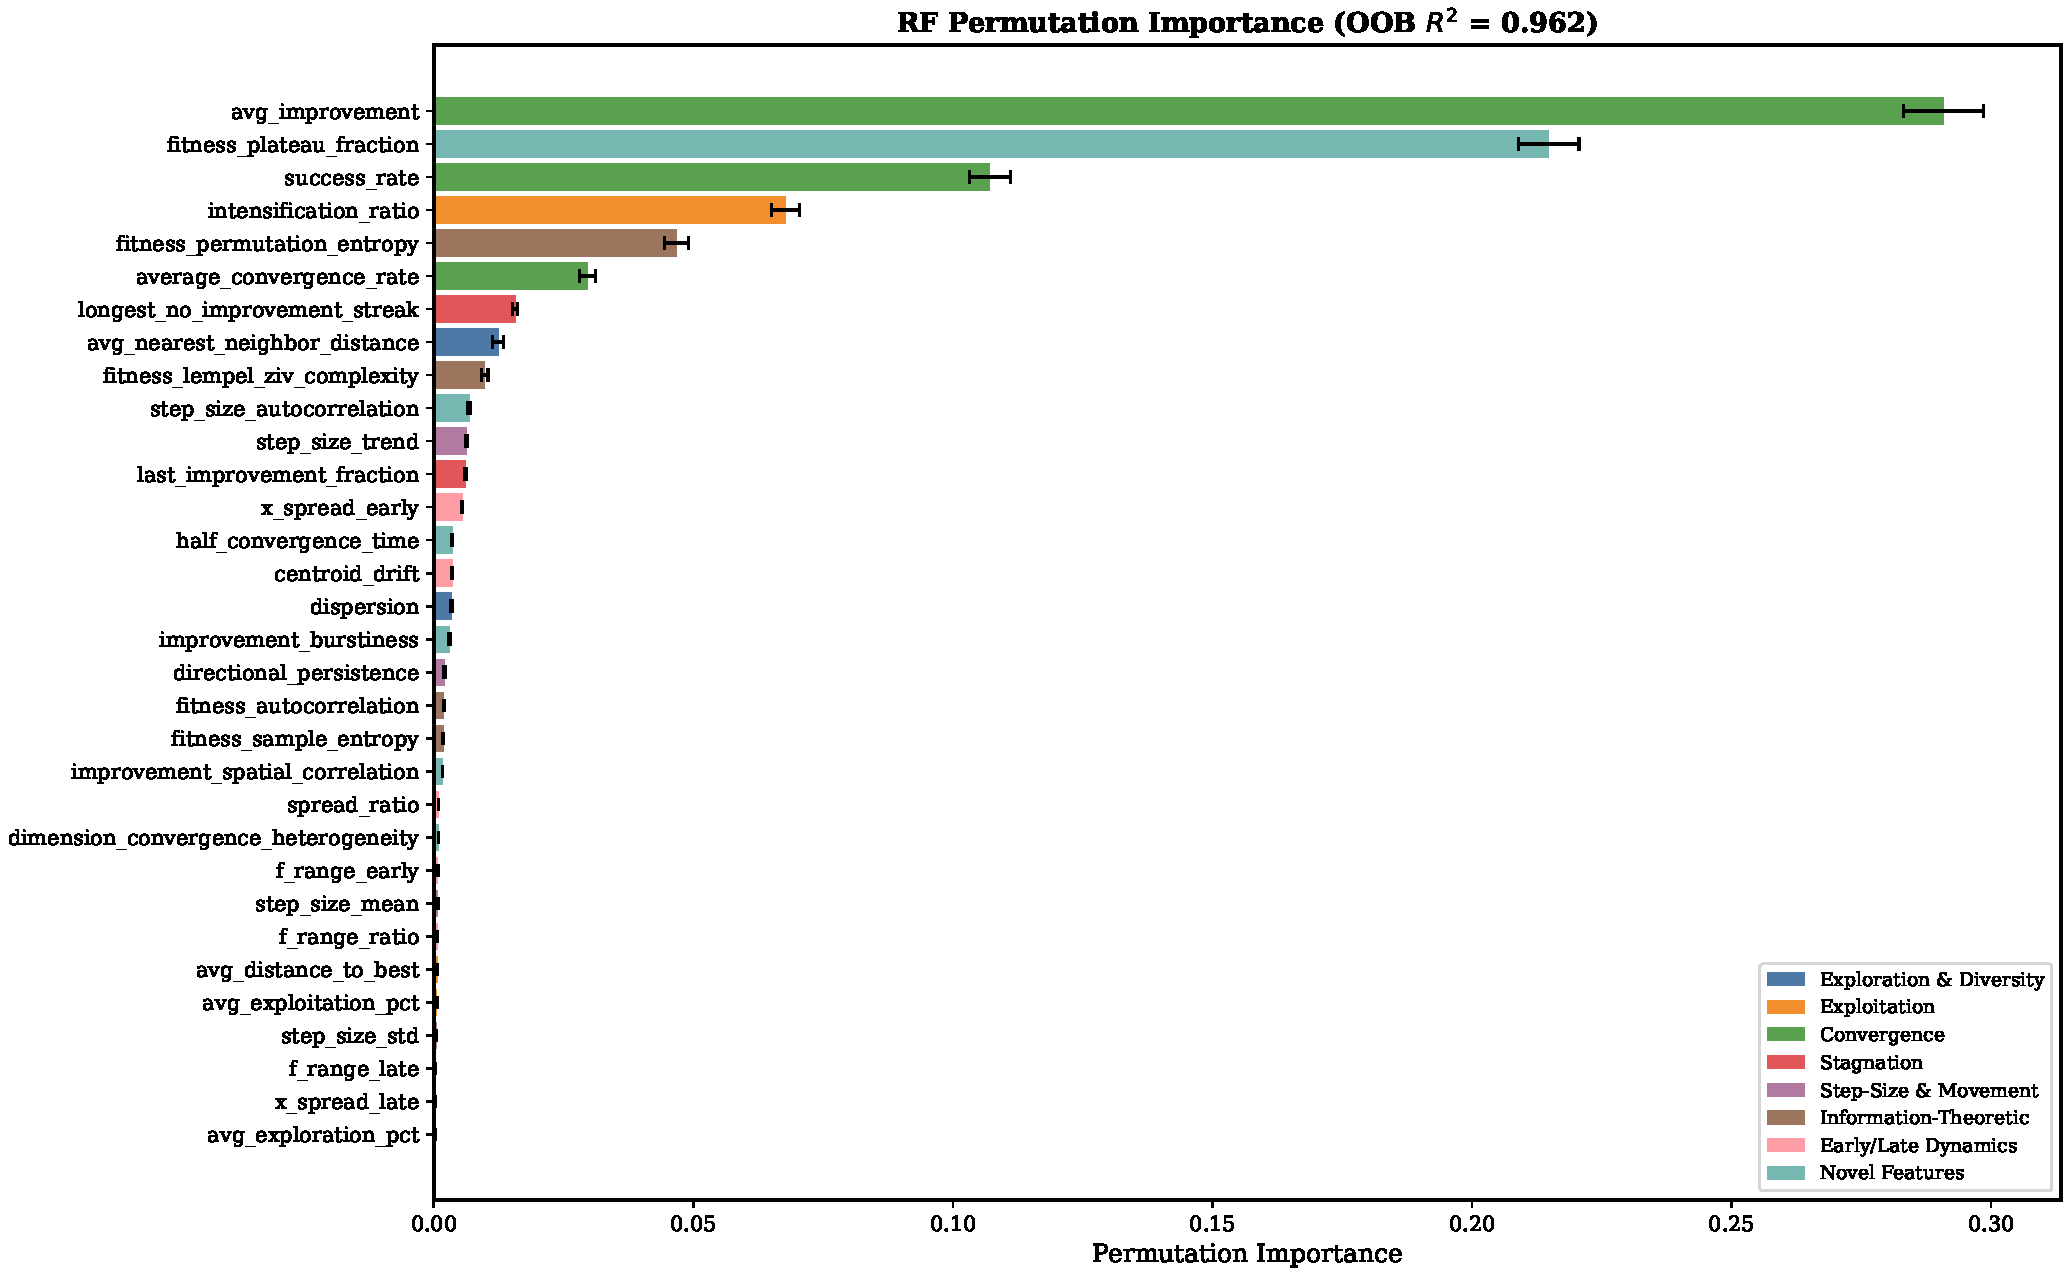
\includegraphics[width=\columnwidth]{figures/fig_rf_importance.pdf}
  \caption{Random Forest permutation importance for all 32 features, sorted by importance. Error bars show standard deviation across 10 permutation repeats.}
  \label{fig:rf-importance}
\end{figure}

\begin{figure}[p]
  \centering
  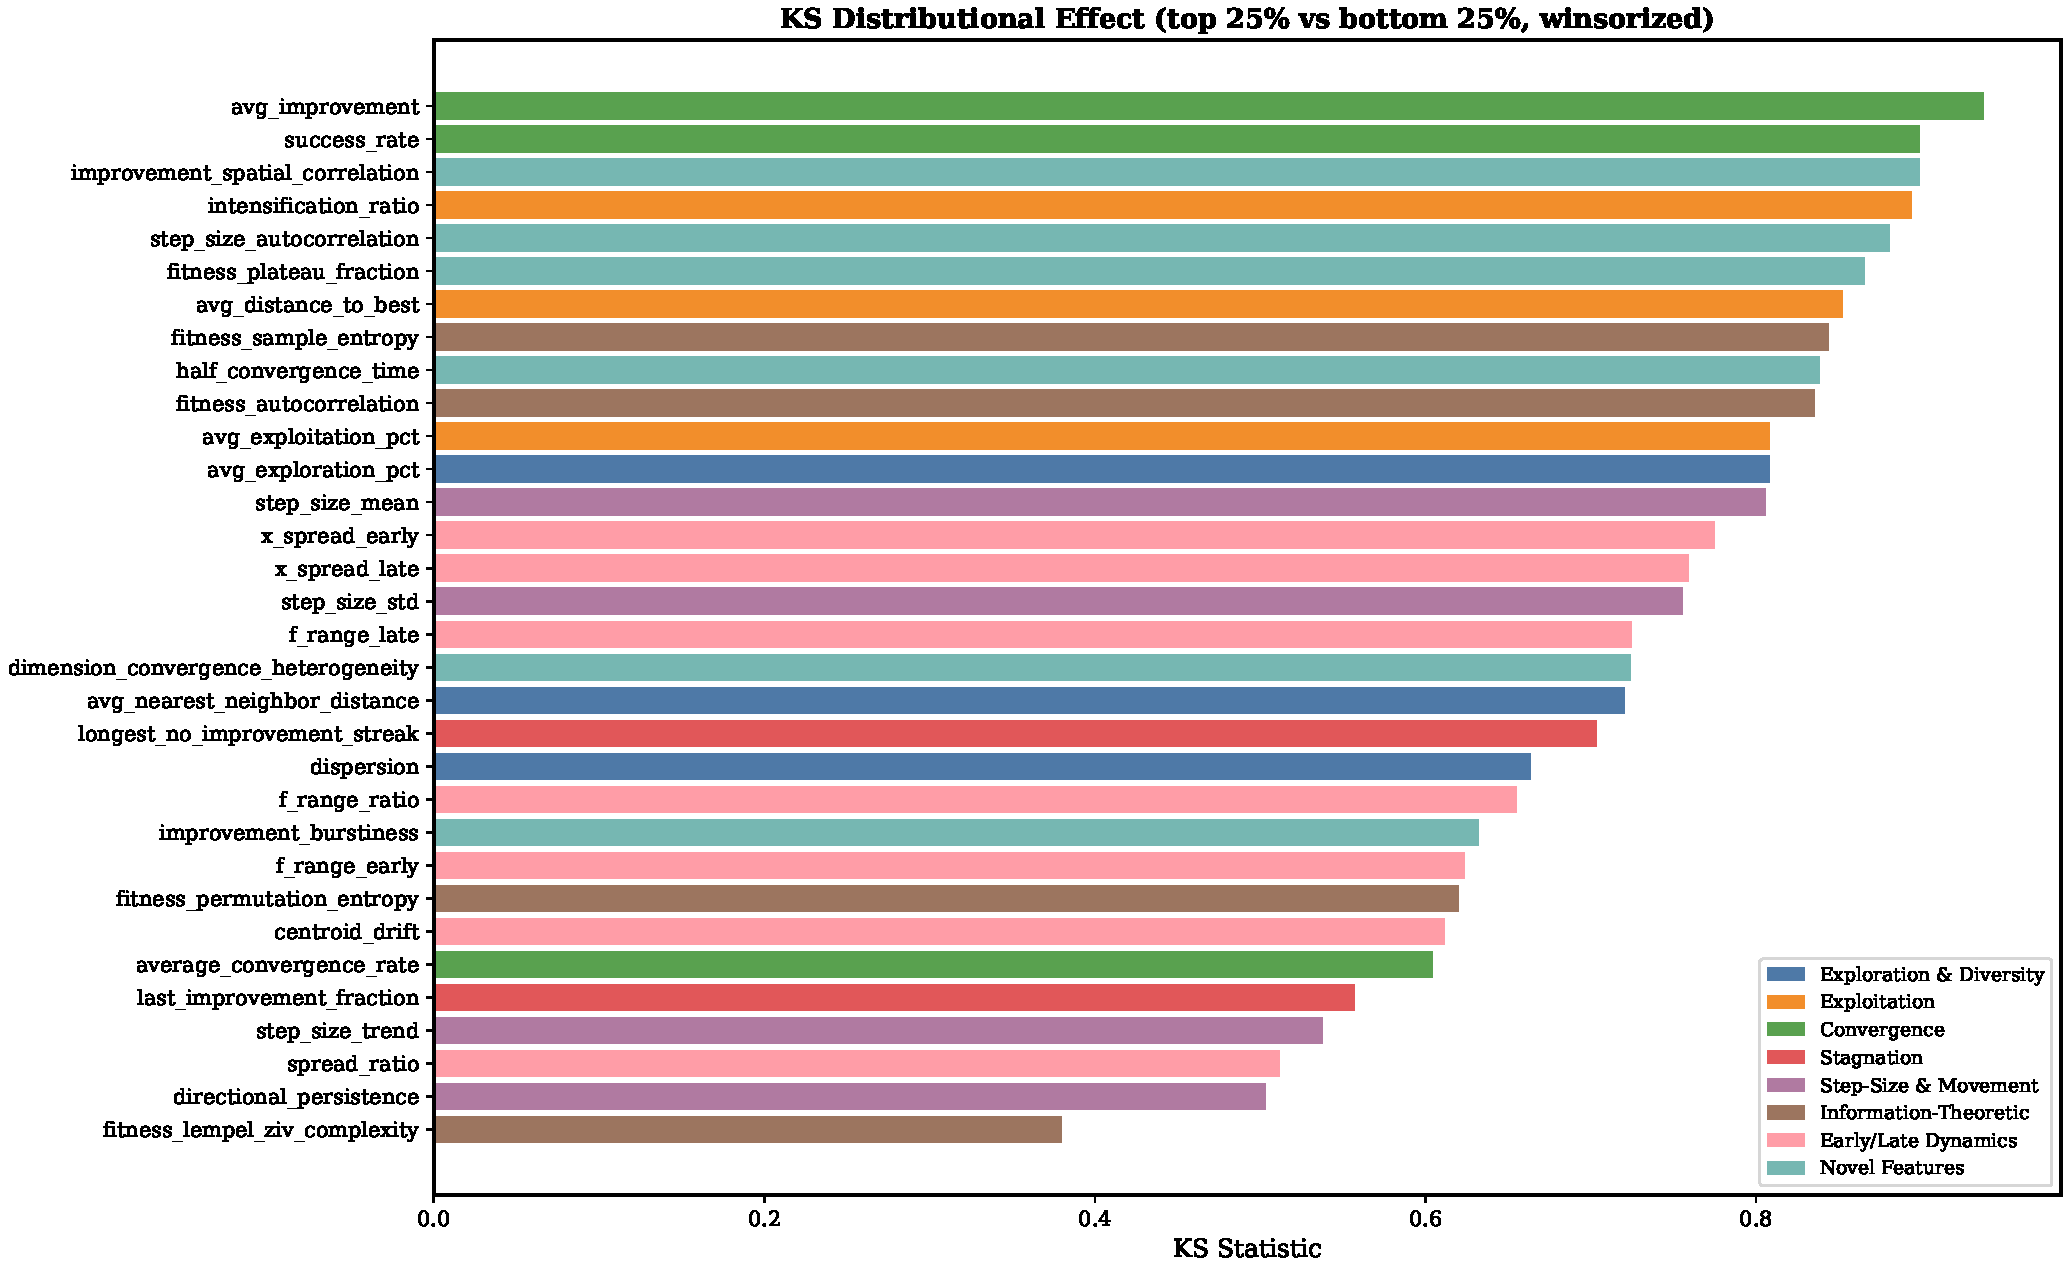
\includegraphics[width=\columnwidth]{figures/fig_ks_effect.pdf}
  \caption{KS distributional effect size between top-25\% and bottom-25\% algorithms by AOCC, sorted by KS statistic. Feature values are winsorized at the 1st/99th percentile before testing.}
  \label{fig:ks-effect}
\end{figure}

\subsection{Distributional Separation}
\label{sec:results-ks}

\Cref{fig:ks-effect} reports the KS statistic for each feature across the $3{,}071$ valid candidates. The KS ranking largely agrees with Spearman on which features matter most, but reveals additional structure. Several features that ranked moderately by Spearman show very high KS values, indicating they separate good from bad algorithms through non-monotonic or threshold effects rather than smooth linear trends. For example, \texttt{avg\_exploitation\_pct} and \texttt{step\_size\_mean} both achieve KS statistics above 0.8 despite more moderate Spearman $|\rho|$ values. At the bottom of the KS ranking, features like \texttt{fitness\_lempel\_ziv\_complexity} and \texttt{spread\_ratio} show weak distributional separation, confirming that they carry little information about algorithm quality regardless of the statistical method used.

\subsection{Consensus Ranking and Selection}
\label{sec:results-selection}

\begin{figure}[!t]
  \centering
  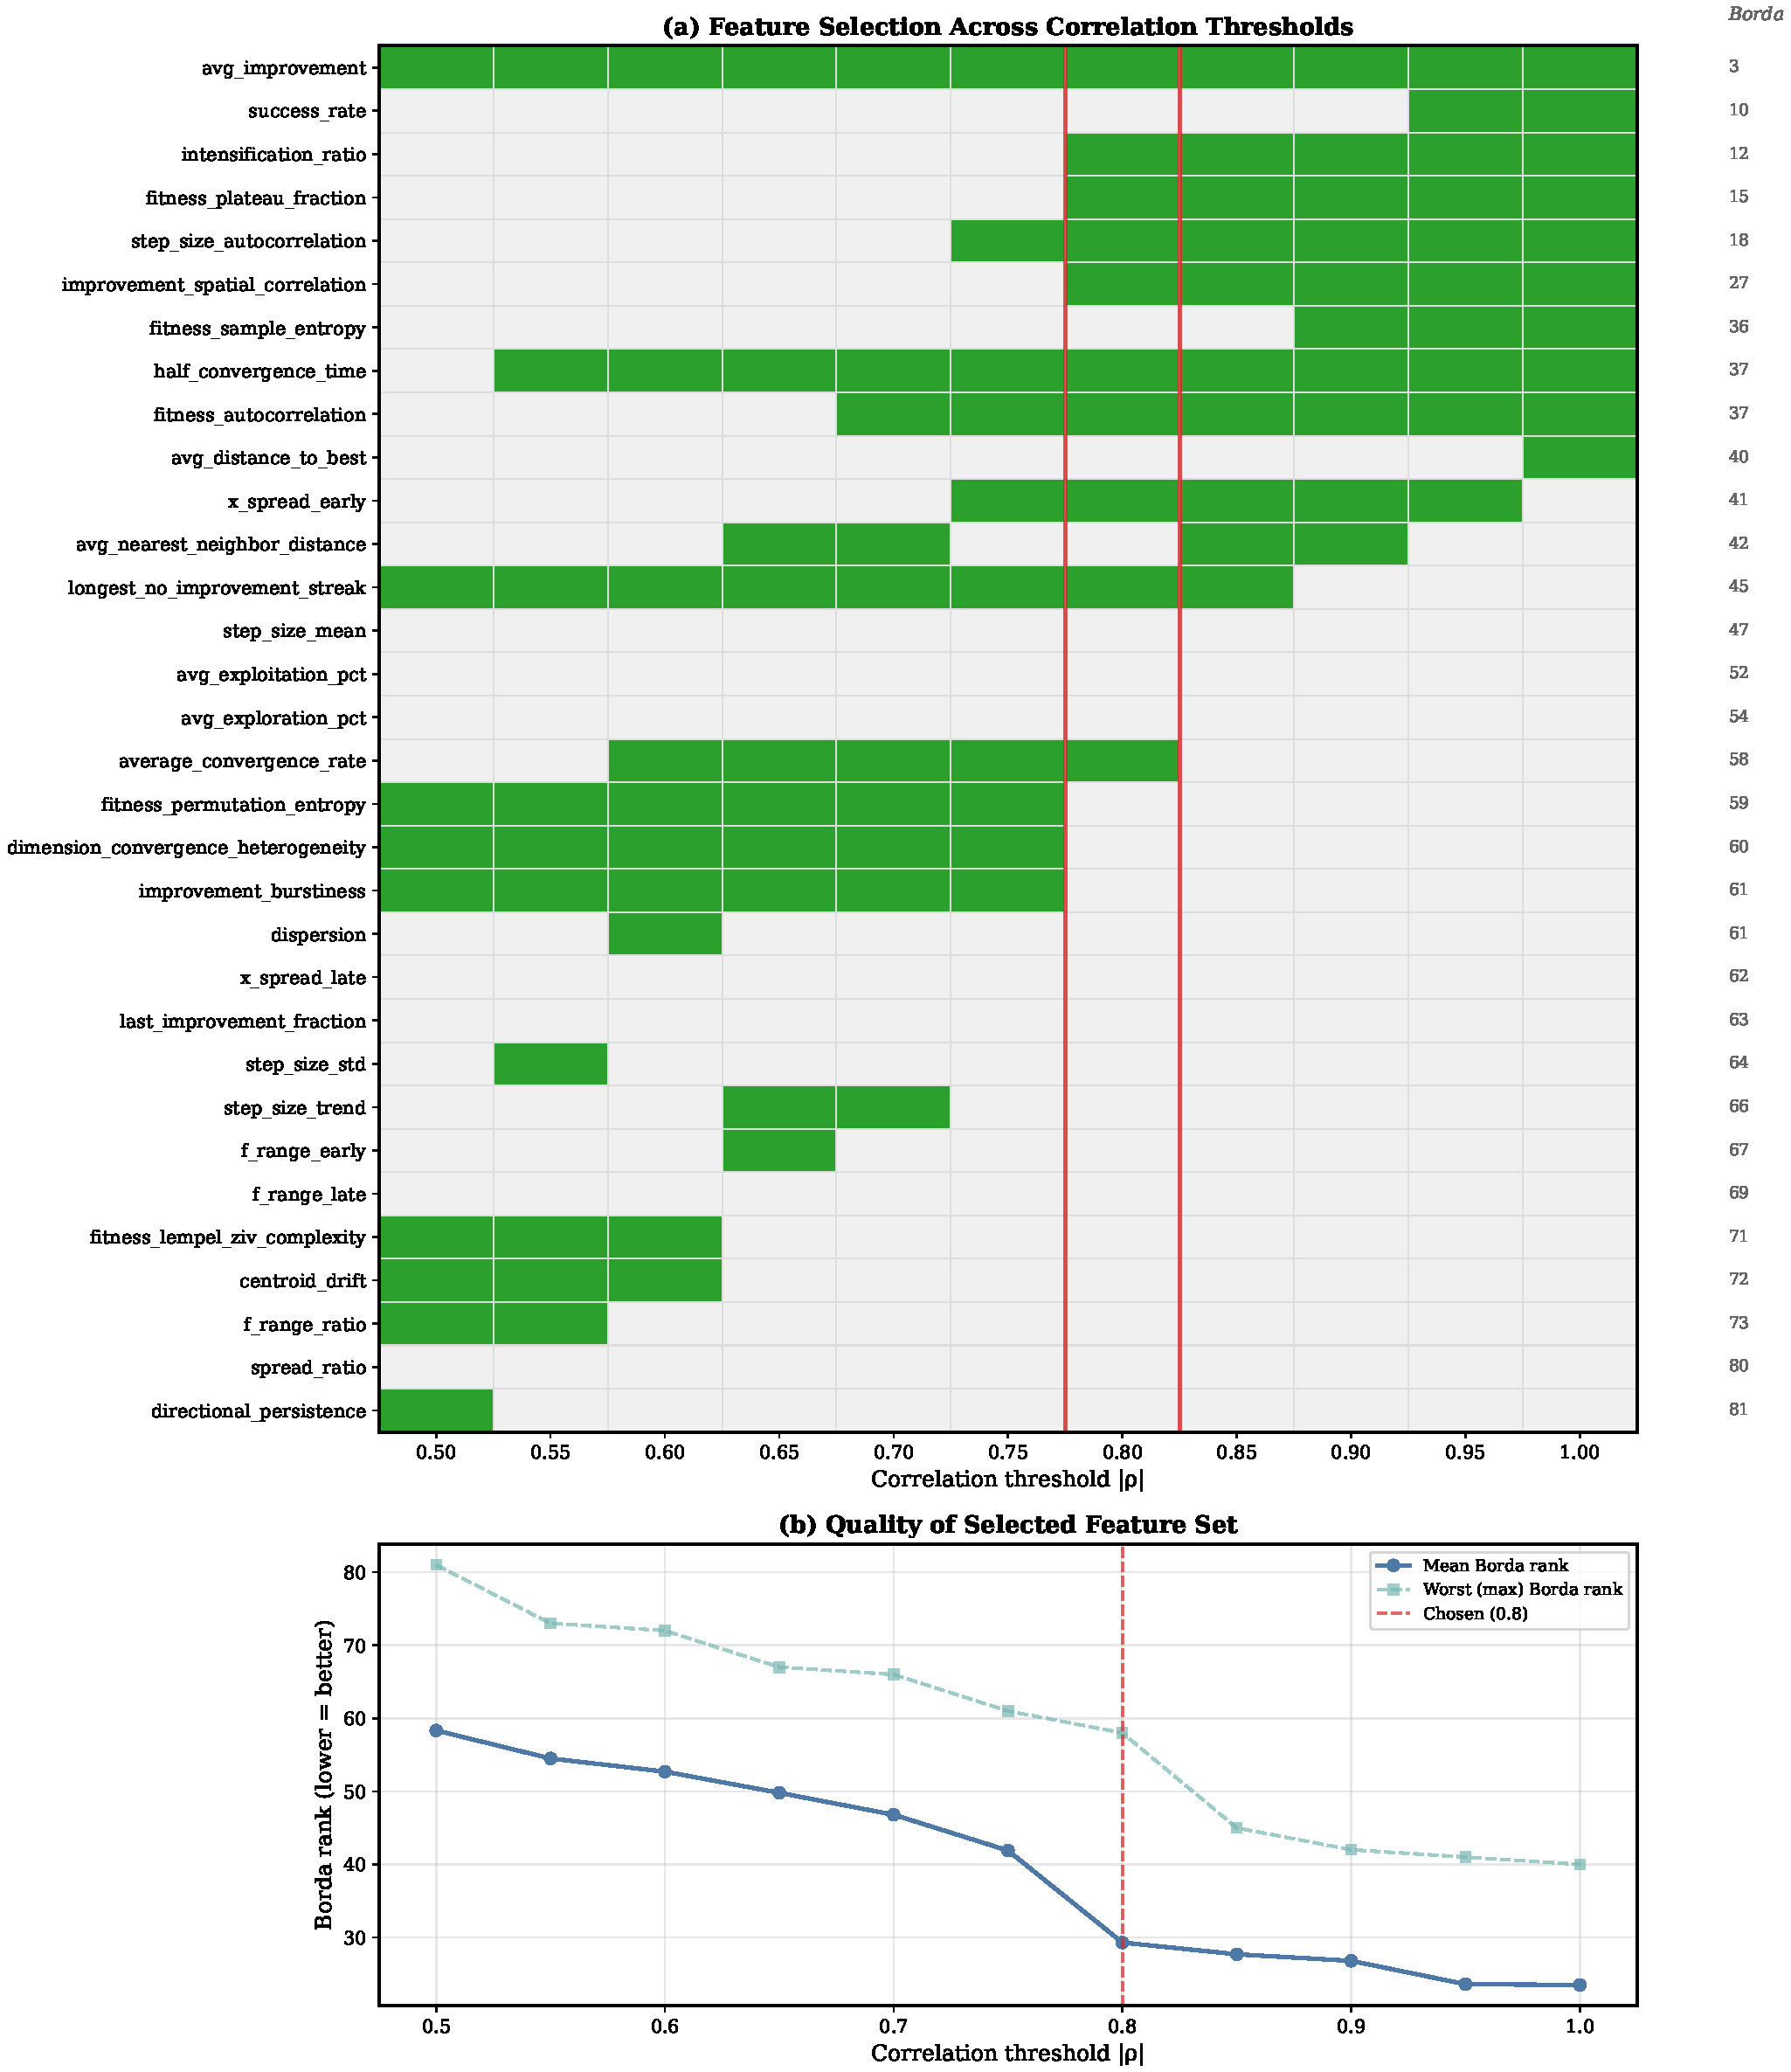
\includegraphics[width=\columnwidth]{figures/fig_feature_sensitivity_combined.pdf}
  \caption{Sensitivity of the 10-feature subset to the redundancy-pruning threshold $\tau$. (a)~Presence heatmap: which of the 32 candidates is selected at each $\tau \in [0.50, 1.00]$ in $0.05$ steps, sorted top-to-bottom by Borda rank. The chosen $\tau = 0.80$ column is highlighted in red. (b)~Mean and worst Borda rank of the selected subset as $\tau$ varies; the dashed line marks the chosen value, which sits at the elbow of the mean curve.}
  \label{fig:feature-sensitivity}

  \vspace{1em}
  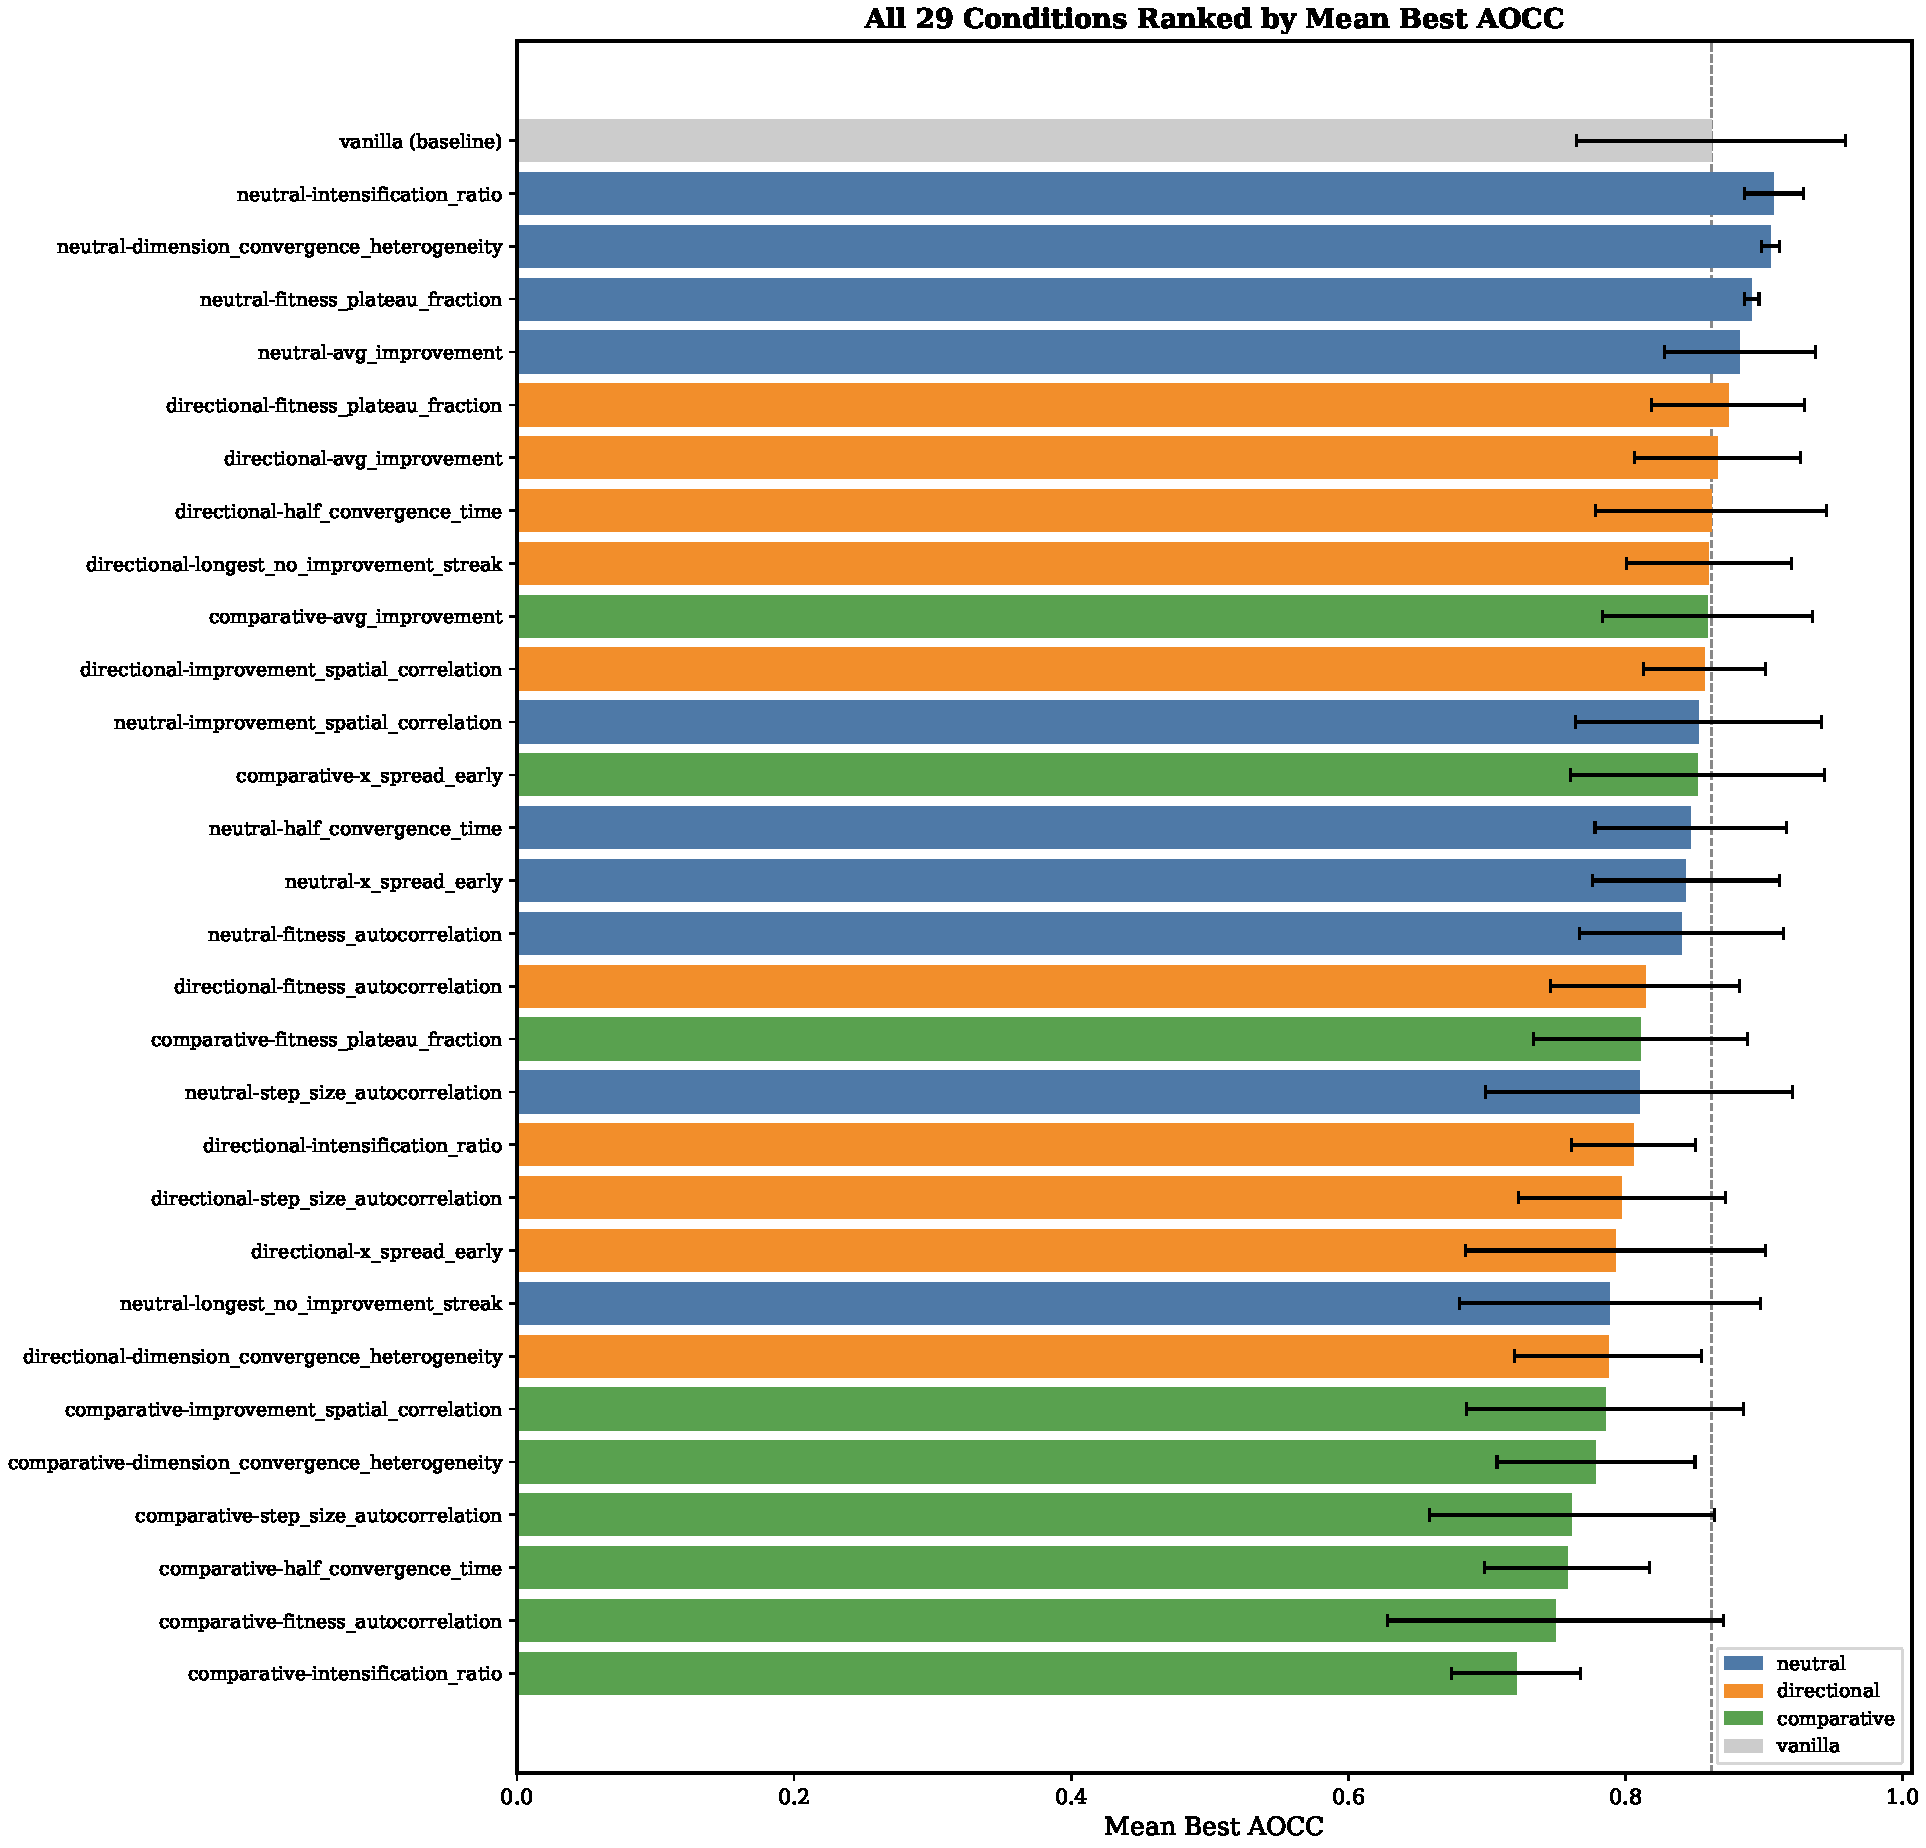
\includegraphics[width=\columnwidth]{figures/fig_condition_ranking.pdf}
  \caption{All 29 conditions ranked by mean best AOCC ($\pm$ std, 5 seeds). Grey bar and dashed line show the vanilla baseline ($0.862$). Colours: blue = neutral, orange = directional, green = comparative.}
  \label{fig:condition-ranking}
\end{figure}

\begin{table*}[p]
\centering
\caption{All 32 behavioural features ranked by Borda consensus. For each method, both the value and rank are shown. The Status column indicates whether a feature was selected for feedback experiments, pruned for redundancy (with the correlated selected feature noted), or not selected.}
\label{tab:feature-consensus}
\footnotesize
\setlength{\tabcolsep}{3.5pt}
\begin{tabular}{@{}rlrrrrrrl@{}}
\toprule
& & \multicolumn{2}{c}{\textbf{Spearman}} & \multicolumn{2}{c}{\textbf{RF Importance}} & \multicolumn{2}{c}{\textbf{KS}} & \\
\cmidrule(lr){3-4} \cmidrule(lr){5-6} \cmidrule(lr){7-8}
\textbf{Borda} & \textbf{Feature} & \boldmath{$\rho$} & \textbf{R} & \textbf{Imp} & \textbf{R} & \textbf{Stat} & \textbf{R} & \textbf{Status} \\
\midrule
3  & avg\_improvement              & $-$.782 &  1 & .291 &  1 & .938 &  1 & \textbf{Selected} \\
7  & success\_rate                 & $+$.766 &  2 & .107 &  3 & .899 &  2 & Pruned ($|r|{=}.92$, avg\_impr) \\
13 & intensification\_ratio        & $+$.725 &  5 & .068 &  4 & .894 &  4 & \textbf{Selected} \\
15 & fitness\_plateau\_frac        & $+$.685 &  7 & .215 &  2 & .867 &  6 & \textbf{Selected} \\
18 & step\_size\_autocorr          & $+$.766 &  3 & .007 & 10 & .881 &  5 & \textbf{Selected} \\
28 & impr\_spatial\_corr           & $+$.757 &  4 & .002 & 21 & .899 &  3 & \textbf{Selected} \\
36 & fitness\_sample\_entropy      & $-$.680 &  8 & .002 & 20 & .845 &  8 & Pruned ($|r|{=}.87$, plateau\_frac) \\
37 & half\_convergence\_time       & $-$.597 & 14 & .004 & 14 & .840 &  9 & \textbf{Selected} \\
38 & fitness\_autocorrelation      & $+$.645 &  9 & .002 & 19 & .835 & 10 & \textbf{Selected} \\
40 & avg\_distance\_to\_best       & $-$.691 &  6 & .001 & 27 & .852 &  7 & Pruned ($|r|{=}.96$, intens\_ratio) \\
40 & x\_spread\_early              & $-$.599 & 13 & .006 & 13 & .775 & 14 & \textbf{Selected} \\
43 & longest\_no\_improv\_streak   & $-$.469 & 16 & .016 &  7 & .703 & 20 & \textbf{Selected} \\
44 & avg\_nn\_distance             & $-$.469 & 17 & .012 &  8 & .720 & 19 & Pruned ($|r|{=}.82$, x\_spread) \\
48 & step\_size\_mean              & $-$.622 & 10 & .001 & 25 & .806 & 13 & Pruned ($|r|{=}.83$, intens\_ratio) \\
52 & avg\_exploitation\_pct        & $+$.612 & 12 & .001 & 28 & .808 & 12 & Pruned ($|r|{=}.87$, intens\_ratio) \\
55 & avg\_exploration\_pct         & $-$.612 & 11 & .000 & 32 & .808 & 12 & Pruned ($|r|{=}.87$, intens\_ratio) \\
55 & dim\_conv\_heterogeneity      & $+$.471 & 15 & .001 & 23 & .727 & 17 & \textbf{Selected} \\
\midrule
55 & average\_convergence\_rate    & $-$.400 & 22 & .030 &  6 & .604 & 27 & --- \\
57 & fitness\_perm\_entropy        & $-$.238 & 27 & .047 &  5 & .622 & 25 & --- \\
58 & dispersion                    & $+$.421 & 21 & .003 & 16 & .664 & 21 & --- \\
64 & improvement\_burstiness       & $+$.370 & 24 & .003 & 17 & .635 & 23 & --- \\
65 & last\_improvement\_frac       & $-$.370 & 25 & .006 & 12 & .555 & 28 & --- \\
65 & step\_size\_std               & $-$.437 & 20 & .001 & 29 & .755 & 16 & --- \\
65 & x\_spread\_late               & $-$.450 & 19 & .000 & 31 & .759 & 15 & --- \\
66 & f\_range\_early               & $-$.466 & 18 & .001 & 24 & .624 & 24 & --- \\
68 & step\_size\_trend             & $-$.228 & 28 & .006 & 11 & .538 & 29 & --- \\
71 & f\_range\_late                & $-$.394 & 23 & .000 & 30 & .724 & 18 & --- \\
71 & centroid\_drift               & $+$.177 & 30 & .004 & 15 & .612 & 26 & --- \\
72 & fitness\_lempel\_ziv          & $+$.152 & 31 & .010 &  9 & .380 & 32 & --- \\
74 & f\_range\_ratio               & $-$.313 & 26 & .001 & 26 & .654 & 22 & --- \\
81 & spread\_ratio                 & $-$.224 & 29 & .001 & 22 & .511 & 30 & --- \\
81 & directional\_persistence      & $+$.139 & 32 & .002 & 18 & .502 & 31 & --- \\
\bottomrule
\end{tabular}
\\[0.3em]
{\scriptsize Borda = sum of ranks (lower is better). R = rank within method. Values are rounded to 3 decimal places. Where features appear tied, ranks reflect the full-precision ordering. Features above the mid-rule were evaluated by the greedy selection and those below were not considered (10 slots already filled). Pruned features show $|r|$ with the correlated selected feature.}
\end{table*}

The redundancy-pruning threshold $\tau$ controls how aggressively the greedy walk discards features that correlate with already-selected ones, and \cref{fig:feature-sensitivity} shows what happens to the selected subset across the swept range $\tau \in [0.50, 1.00]$ at an intervals of $0.05$. The top panel reports which of the 32 candidates survives at each $\tau$, sorted by Borda rank. The bottom panel tracks the mean and worst Borda rank of the selected subset as $\tau$ varies. Top-ranked features remain stable across the full range, while features lower in the Borda order swap in and out with small threshold changes. Tightening past $\tau = 0.80$ admits lower-Borda candidates and inflates the worst Borda rank in the subset. Loosening below $\tau = 0.80$ prunes features that still carry complementary signal. The mean Borda rank shows its largest single-step improvement at the $0.75$ to $0.80$ transition and plateaus thereafter, motivating $\tau = 0.80$ as the elbow of the quality--threshold curve.

\Cref{tab:feature-consensus} presents all 32 features with their per-method values and ranks, sorted by Borda consensus score. The final set comprises three BLADE features and seven newly introduced features from this thesis, validating the feature design effort described in \cref{ch:features}. \Cref{tab:feature-consensus} reveals that \texttt{intensification\_ratio} alone makes four other metrics redundant, including two BLADE exploration/exploitation percentages and the widely used \texttt{avg\_distance\_to\_best}. Several features with strong individual method rankings fail the consensus. For example, \texttt{fitness\_permutation\_entropy} ranks 5th by RF importance but only 27th by Spearman.

% ===========================================================================
\section{Behavioural Feedback}
\label{sec:results-feedback}

The Stage~3 dataset contains $14{,}127$ valid candidates produced by Gemini~3 Flash across 29 feedback conditions (10 features $\times$ 3 framings, minus the comparative version of \texttt{longest\_no\_improvement\_streak} excluded for non-monotonicity) with 5 independent seeds per condition. This section compares the three feedback formats against each other and against the vanilla AOCC-only baseline, then examines how reliably each format steers behaviour toward the prescribed direction and how the underlying feature--AOCC signal shifts between Stage~1 and Stage~3.

\begin{table*}[!t]
\centering
\caption{Behavioural steering results per feature. For each format: mean best AOCC ($\pm$ std) and median behavioural feature value ($\pm$ std). The final columns show whether directional/comparative shifted the feature toward the advised direction relative to neutral.}
\label{tab:steering-detail}
\footnotesize
\setlength{\tabcolsep}{3.5pt}
\begin{tabular}{@{}lr|rr|rr|rr|cc@{}}
\toprule
& & \multicolumn{2}{c|}{\textbf{Neutral}} & \multicolumn{2}{c|}{\textbf{Directional}} & \multicolumn{2}{c|}{\textbf{Comparative}} & \multicolumn{2}{c}{\textbf{Steered}} \\
\textbf{Feature} & \textbf{Adv.} & \textbf{AOCC} & \textbf{Feat.} & \textbf{AOCC} & \textbf{Feat.} & \textbf{AOCC} & \textbf{Feat.} & \textbf{D} & \textbf{C} \\
\midrule
avg\_impr      & $\downarrow$ & \textbf{.883$\pm$.054} & .094$\pm$.198 & .866$\pm$.060 & .105$\pm$.206 & .860$\pm$.076 & .104$\pm$.237 & $\times$ & $\times$ \\
intens\_ratio  & $\uparrow$   & \textbf{.907$\pm$.021} & .813$\pm$.213 & .806$\pm$.044 & .783$\pm$.125 & .721$\pm$.046 & .852$\pm$.189 & $\times$ & $\checkmark$ \\
plateau\_frac  & $\uparrow$   & \textbf{.891$\pm$.005} & .448$\pm$.210 & .874$\pm$.055 & .364$\pm$.177 & .811$\pm$.077 & .553$\pm$.210 & $\times$ & $\checkmark$ \\
step\_autocorr & $\uparrow$   & \textbf{.810$\pm$.111} & .897$\pm$.111 & .797$\pm$.075 & .863$\pm$.123 & .761$\pm$.103 & .877$\pm$.135 & $\times$ & $\times$ \\
impr\_spatial  & $\uparrow$   & .853$\pm$.089 & .649$\pm$.091 & \textbf{.857$\pm$.044} & .630$\pm$.107 & .786$\pm$.100 & .629$\pm$.092 & $\times$ & $\times$ \\
half\_conv     & $\downarrow$ & .847$\pm$.069 & .003$\pm$.007 & \textbf{.862$\pm$.083} & .001$\pm$.004 & .758$\pm$.060 & .003$\pm$.022 & $\checkmark$ & $\times$ \\
fit\_autocorr  & $\uparrow$   & \textbf{.840$\pm$.074} & .718$\pm$.092 & .814$\pm$.068 & .753$\pm$.128 & .749$\pm$.121 & .790$\pm$.140 & $\checkmark$ & $\checkmark$ \\
x\_spread      & $\downarrow$ & .844$\pm$.067 & 1.55$\pm$.562 & .793$\pm$.108 & 0.55$\pm$.451 & \textbf{.852$\pm$.092} & 0.74$\pm$.443 & $\checkmark$ & $\checkmark$ \\
longest\_str   & $\downarrow$ & .789$\pm$.109 & 849$\pm$1762  & \textbf{.860$\pm$.059} & 1028$\pm$2351 & \multicolumn{2}{c|}{---} & $\times$ & --- \\
dim\_conv\_het & $\uparrow$   & \textbf{.905$\pm$.006} & .050$\pm$.052 & .788$\pm$.068 & .007$\pm$.056 & .779$\pm$.071 & .034$\pm$.168 & $\times$ & $\times$ \\
\midrule
\multicolumn{8}{@{}l}{Steering accuracy} & 3/10 & 4/9 \\
\bottomrule
\end{tabular}
\\[0.3em]
{\scriptsize Adv. = direction associated with higher AOCC from Spearman analysis ($\uparrow$/$\downarrow$). AOCC = mean best across 5 seeds. Feat. = median behavioural feature value across all valid candidates. $\checkmark$/$\times$ = shifted toward/away from advised direction relative to neutral.}
\end{table*}

\begin{figure*}[t]
  \centering
  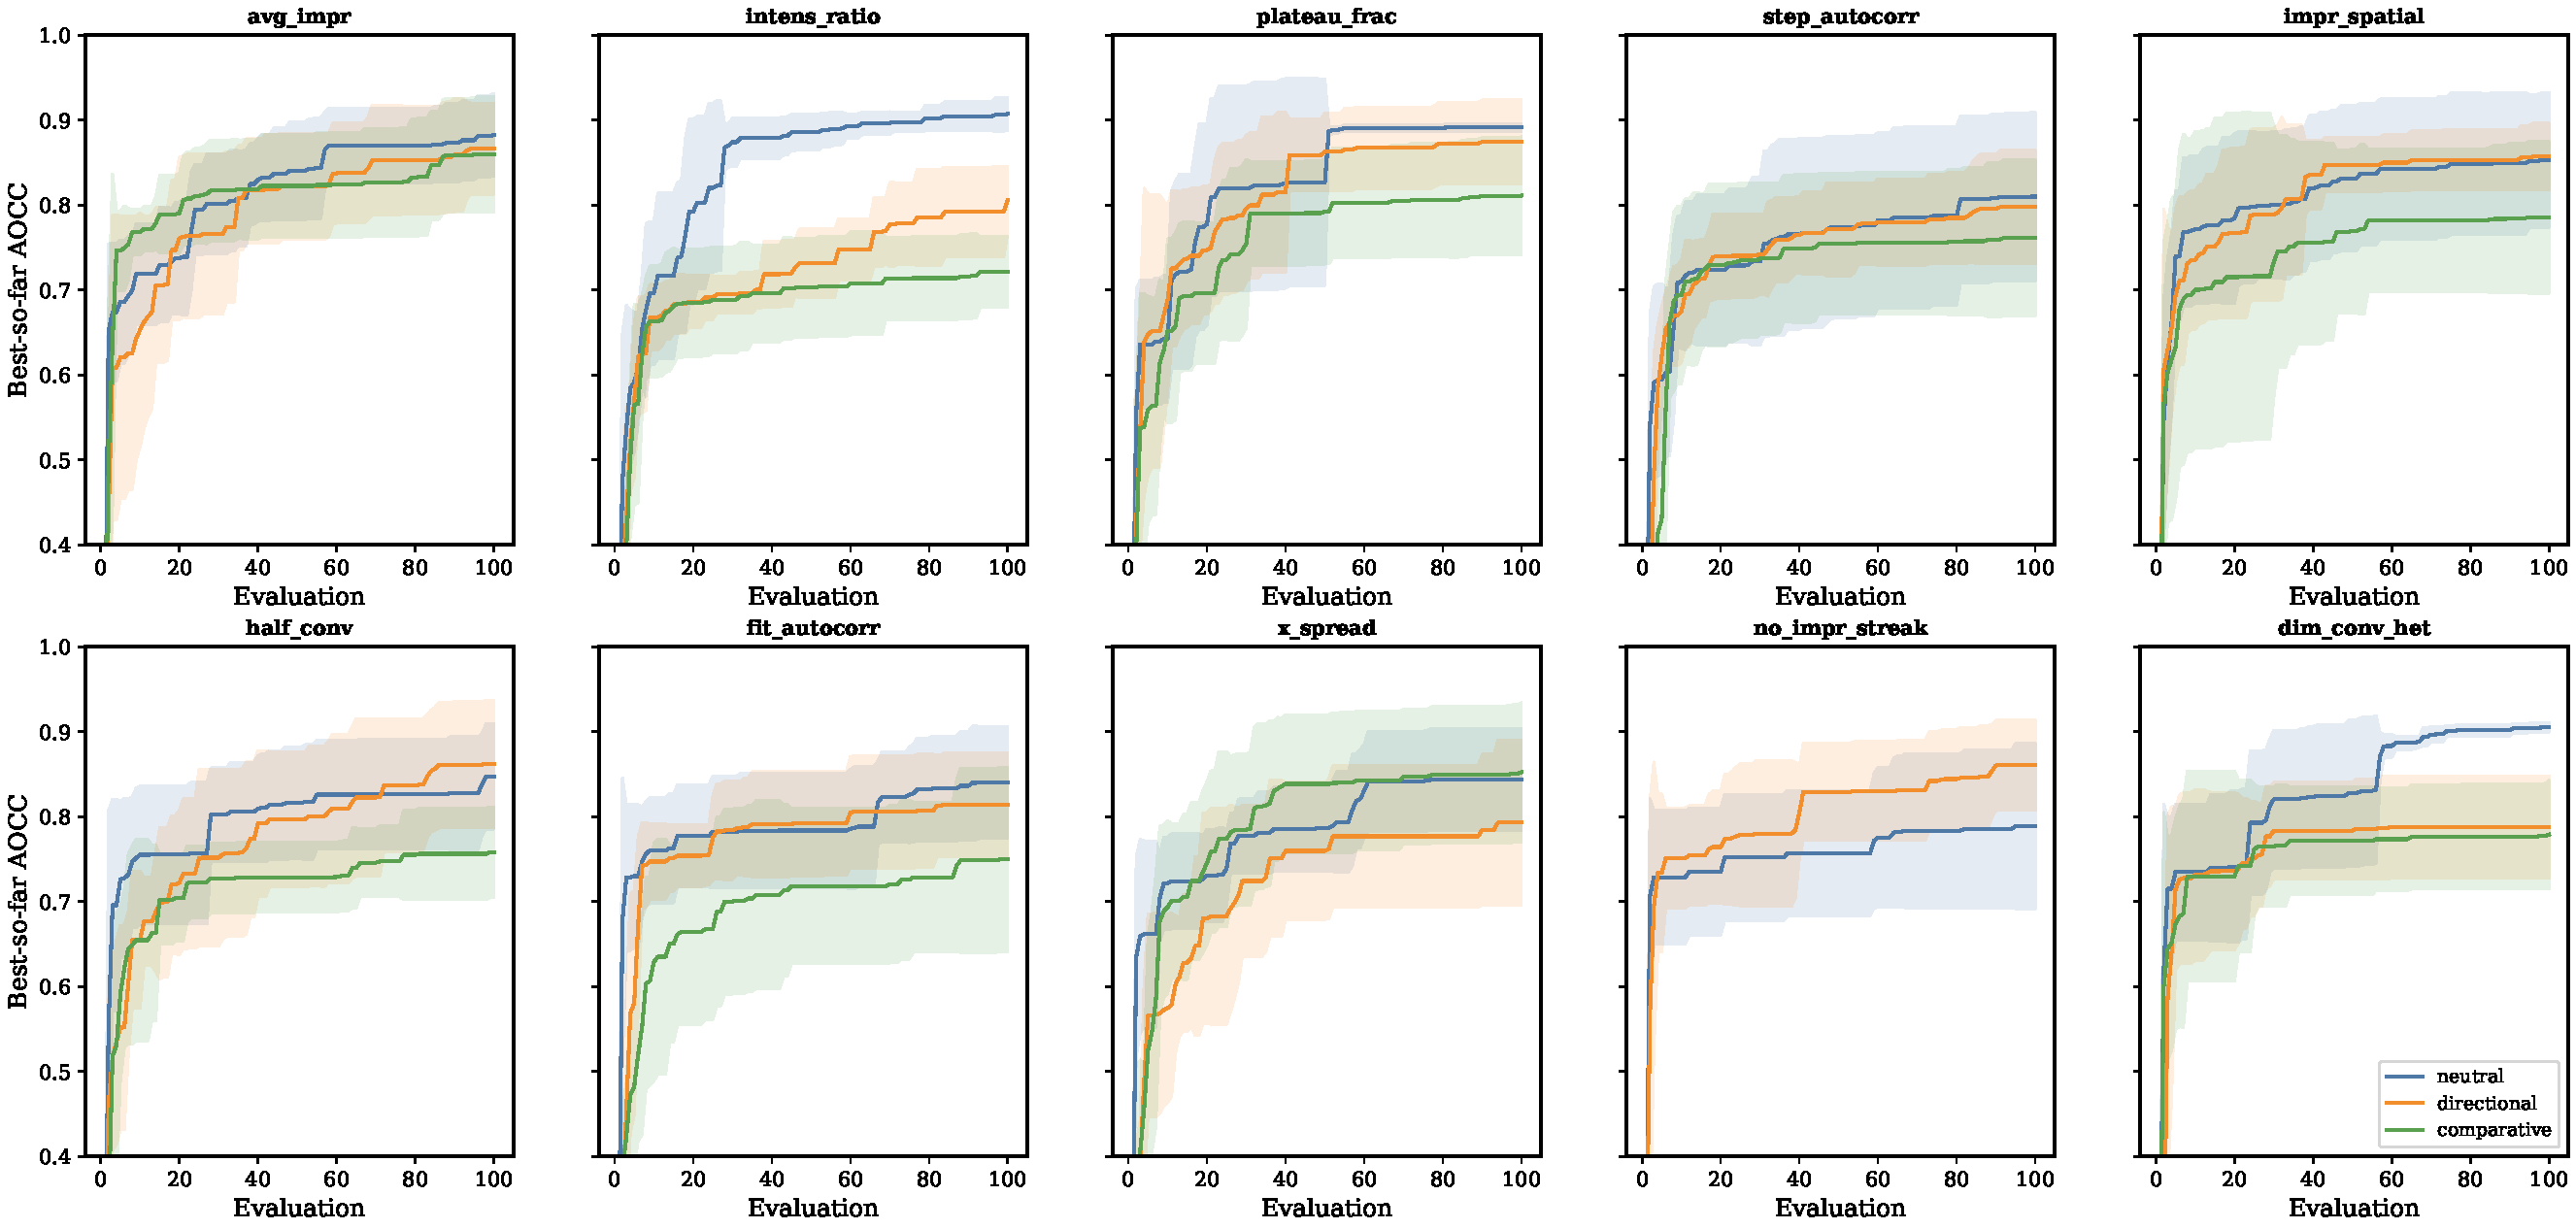
\includegraphics[width=\textwidth]{figures/fig_convergence_by_format.pdf}
  \caption{Best-so-far AOCC over 100 evaluations for each feature, split by feedback format (mean $\pm$ 1 std, 5 seeds). Neutral (blue) typically converges fastest and highest.}
  \label{fig:convergence-by-format}
\end{figure*}

\subsection{Format Ranking}
\label{sec:results-format-ordering}

\Cref{fig:condition-ranking} ranks all 29 conditions by mean best AOCC alongside the vanilla baseline. The top four conditions are all neutral format, and a clear pattern emerges. Neutral conditions cluster at the top, directional in the middle, and comparative at the bottom. To test whether this ordering reflects a genuine difference rather than sampling noise, we apply the Kruskal--Wallis test~\cite{kruskal1952ranks}, a non-parametric alternative to one-way ANOVA that compares the rank distributions of independent groups without assuming normality. The test treats the per-(format, feature) mean AOCCs as independent samples within each format, ignoring the fact that the same feature set appears across formats. A paired Friedman test would be more rigorous, but is complicated by comparative's missing feature. The test confirms a significant difference among formats ($H = 11.5$, $p = 0.003$), with neutral achieving a mean AOCC of $0.855$, directional $0.827$, and comparative $0.784$. The AOCC columns in \cref{tab:steering-detail} show this pattern per feature, with the best format highlighted in bold. Neutral produces the best AOCC for 6 of 10 features, directional for 3, and comparative for just 1. Neutral conditions also have the highest failure rate at $3.5\%$ compared to $2.6\%$ for directional and $1.5\%$ for comparative.

Some behavioural features clearly reduce performance regardless of feedback format. In particular \texttt{step\_size\_autocorrelation}, where even the best format (neutral) achieves only $0.810$. Comparative feedback leads to a reduction in performance relative to neutral for 8 of 9 features, with \texttt{x\_spread\_early} ($+0.008$) being the sole exception. Directional feedback shows more variance. For 6 features it stays within $0.02$ of neutral or beats it outright, while for other 4 it produces drops of $-0.026$ to $-0.117$.

\subsection{Statistical Significance}
\label{sec:results-significance}

Six conditions exceed the vanilla baseline AOCC of $0.862$, four neutral (\texttt{intensification\_ratio}, \texttt{dim\_conv\_heterogeneity}, \texttt{plateau\_fraction}, \texttt{avg\_improvement}) and two directional (\texttt{plateau\_fraction}, \texttt{avg\_improvement}), with \texttt{neutral-intensification\_ratio} at $0.907 \pm 0.021$ performing the best. None of these reach statistical significance against vanilla, and the failure can be attributed to the low number of seeds per condition. With only 5 seeds per group, the Mann--Whitney $U$ test (the two-group form of the Kruskal--Wallis test used above) has limited resolution. There are $\tfrac{10!}{(5!)^2} = 252$ possible ways to interleave the two groups' ranks, so the smallest two-tailed p-value the test can ever produce is $2/252 \approx 0.008$. That minimum is reached only when the two distributions are completely separated, meaning every value in one group exceeds every value in the other. The expected min and max of $n = 5$ samples from a normal distribution sit about $\pm 1.16\,\sigma$ from the mean,\footnote{$1.16 \approx E[X_{(5:5)}]$, the expected value of the largest order statistic in a sample of five standard-normal draws; Blom's approximation $\Phi^{-1}((n - 3/8)/(n + 1/4))$ gives $1.18$ for $n=5$, close to the tabulated value $1.163$.} so separation between vanilla (seed-to-seed AOCC std $\sigma_v = 0.108$) and the best performing condition \texttt{neutral-intensification\_ratio} ($\sigma_b = 0.021$) requires a mean gap exceeding roughly $1.16\,(\sigma_v + \sigma_b) \approx 0.15$. The observed $+0.045$ gap is well below this threshold and the two distributions overlap substantially, so the test cannot rule out chance even though the direction is consistent. Doubling to 10 seeds per condition, as in the Stage~4 setup, raises the number of rank interleavings to $\tfrac{20!}{(10!)^2} = 184{,}756$ and shrinks the minimum detectable effect size by roughly $1/\sqrt{2}$, bringing gaps near the observed $+0.045$ within reach. The seed budget itself was constrained by Gemini API costs. The 29-condition feature$\times$format sweep at 100 candidates per seed already amounts to $14{,}500$ LLaMEA iterations, and doubling to 10 seeds would have cost $29{,}000$ iterations, larger than the entire Stage~4 budget reserved for the head-to-head comparison.

When comparing the three feedback formats against each other for a single behavioural feature, two features do reach statistical significance. With three groups of $n = 5$, the Kruskal--Wallis test has $\tfrac{15!}{(5!)^3} = 756{,}756$ distinct rank assignments and the achievable minimum p-value drops by several orders of magnitude. For \texttt{intensification\_ratio}, neutral ($0.907$) outperforms directional ($0.806$) and comparative ($0.721$) with complete pairwise separation across seeds (Cliff's $d = 1.0$ for every pairwise comparison, Kruskal--Wallis $p = 0.002$). The same holds for \texttt{dim\_conv\_heterogeneity}, where neutral ($0.905$) outperforms directional ($0.788$) and comparative ($0.779$) with no overlap between neutral and either prescriptive format ($d = 1.0$ pairwise, $p = 0.009$).

\subsection{Convergence Dynamics}
\label{sec:results-convergence}

\begin{table*}[t]
\centering
\caption{Feature--AOCC relationship shift from Stage~1 (all models, $n{=}3{,}086$) to Stage~3 (Gemini Flash only, $n{=}14{,}127$). Tier columns show median feature values for bottom-25\% and top-10\% algorithms by AOCC in each stage.}
\label{tab:correlation-shift}
\footnotesize
\begin{tabular}{@{}l|rrrr|rrrr|l@{}}
\toprule
& \multicolumn{4}{c|}{\textbf{Stage 1 (all models)}} & \multicolumn{4}{c|}{\textbf{Stage 3 (Gemini Flash)}} & \\
\textbf{Feature} & \boldmath{$\rho$} & \textbf{Bot25} & \textbf{Top10} & \textbf{Gap} & \boldmath{$\rho$} & \textbf{Bot25} & \textbf{Top10} & \textbf{Gap} & \textbf{Dir.} \\
\midrule
avg\_impr       & $-$.782 & 1.752 & 0.093 & 1.659 & $-$.184 & 0.136 & 0.078 & 0.059 & same \\
intens\_ratio   & $+$.725 & 0.000 & 0.879 & 0.879 & $+$.475 & 0.714 & 0.873 & 0.160 & same \\
plateau\_frac   & $+$.689 & 0.000 & 0.597 & 0.597 & $+$.578 & 0.183 & 0.597 & 0.414 & same \\
step\_autocorr  & $+$.764 & 0.130 & 0.910 & 0.780 & $+$.468 & 0.822 & 0.903 & 0.082 & same \\
impr\_spatial   & $+$.757 & 0.087 & 0.682 & 0.595 & $+$.446 & 0.615 & 0.689 & 0.073 & same \\
half\_conv      & $-$.611 & 0.010 & 0.001 & 0.009 & $-$.640 & 0.003 & 0.001 & 0.002 & same \\
fit\_autocorr   & $+$.650 & 0.003 & 0.766 & 0.764 & $+$.138 & 0.720 & 0.738 & 0.018 & same \\
x\_spread       & $-$.570 & 2.889 & 0.621 & 2.268 & $-$.410 & 1.608 & 0.578 & 1.030 & same \\
longest\_str    & $-$.427 & 6282  & 5543  & 739   & $+$.495 & 1499  & 6018  & 4520  & \textbf{flip} \\
dim\_conv\_het  & $+$.424 & 0.001 & 0.081 & 0.080 & $+$.167 & 0.049 & 0.089 & 0.040 & same \\
\bottomrule
\end{tabular}
\\[0.3em]
{\scriptsize Bot25/Top10 = median feature value among bottom-25\%/top-10\% algorithms by AOCC. Gap = $|$Top10 $-$ Bot25$|$. Dir. = whether correlation direction is preserved.}
\end{table*}

\Cref{fig:convergence-by-format} shows the best-so-far convergence curves for each feature, split by format. The two features with the strongest format effects, \texttt{intensification\_ratio} and \texttt{dim\_conv\_heterogeneity} (the same pair that reach within-feature statistical significance above), show a clear separation early in the run that widens throughout. The features where directional performs well (\texttt{half\_convergence\_time}, \texttt{longest\_streak}) show the formats tracking closely, consistent with the small AOCC deltas reported above. For features like \texttt{average\_improvement}, all three formats converge to similar levels with high variance, showing that this feature does not strongly differentiate performance regardless of how feedback is framed.

\subsection{Behavioural Drift Between Stages}
\label{sec:results-drift}

To validate whether the directional advice itself remains correct in the Stage~3 context, we recompute Spearman correlations between each feature and AOCC on the Stage~3 dataset (\cref{tab:correlation-shift}). Since Stage~3 uses only Gemini~3 Flash, the mean AOCC is higher ($0.646$ vs $0.484$ in Stage~1) and the performance range is narrower. Despite this, 9 of 10 features maintain the same correlation direction, confirming that directional advice is empirically sound.

The correlation magnitudes tell a more nuanced story. Most features weaken substantially, with \texttt{avg\_improvement} showing the most dramatic drop from $\rho = -0.782$ (the strongest correlation in Stage~1) to just $-0.184$ in Stage~3. Only one feature, \texttt{half\_convergence\_time}, strengthens its correlation in the same direction ($-0.611$ to $-0.640$). \texttt{longest\_no\_improvement\_streak} ($-0.427$ to $+0.495$) increases in magnitude but reverses sign, consistent with the non-monotonic relationship that motivated its exclusion from comparative feedback. The reversal points to a broader observation about the pipeline rather than a flaw isolated to this one feature. Everything upstream of Stage~3, both the feature selection in \cref{sec:results-features} and the directional/comparative reference values, was derived from the Stage~1 dataset spanning all 10 models. The 10 features carried forward were chosen because they predicted AOCC across that heterogeneous population, and the prescriptive advice attached to each was calibrated against the same data. When Stage~3 deploys only Gemini~3 Flash, features whose Stage~1 signal was driven mostly by the weaker models retain less predictive power for Flash specifically, and the steering advice inherits some of that mismatch. \texttt{longest\_no\_improvement\_streak} is the most extreme case, but the broader magnitude shrinkage in \cref{tab:correlation-shift} is consistent with a milder version of the same effect operating across many features. The Stage~1 reference remains a reasonable starting point given the cost of running a fresh model-specific screen, but the results suggest that target-model calibration of both feature selection and prescriptive advice would tighten the signal that prescriptive feedback attempts to convey.

\subsection{Behaviour Steering}
\label{sec:results-decoupling}

\begin{figure*}[!t]
  \centering
  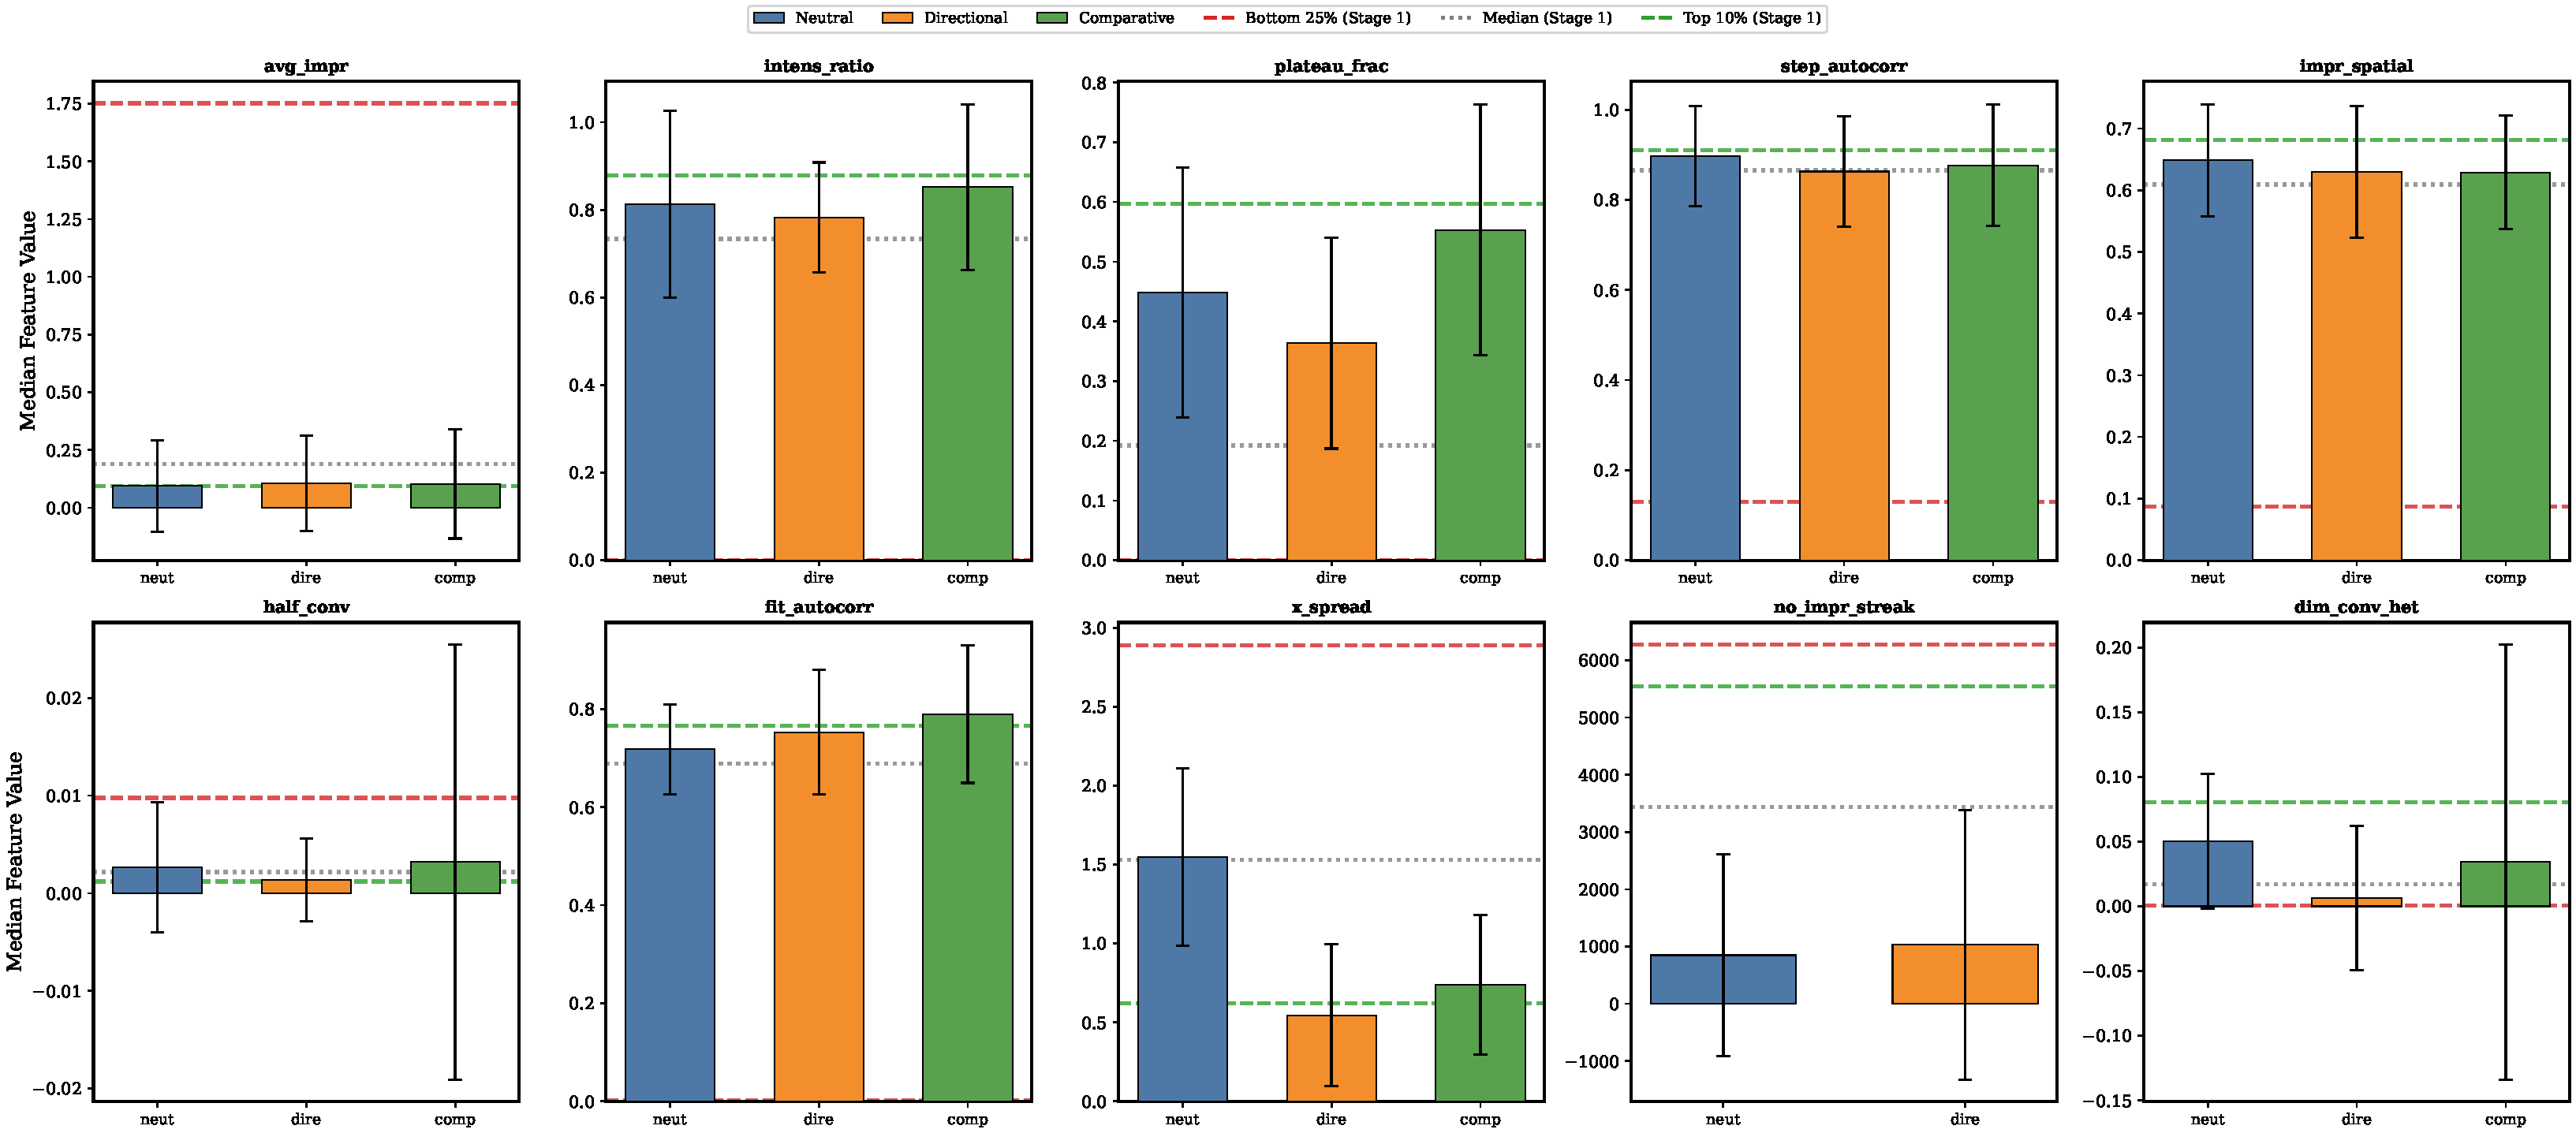
\includegraphics[width=\textwidth]{figures/fig_guided_medians.pdf}
  \caption{Median behavioural feature value by feedback format (bars) compared against Stage~1 AOCC performance tiers (dashed lines): bottom-25\% (red), median (grey), and top-10\% (green). Reference values are computed from all Stage~1 candidates, independent of the feedback experiments.}
  \label{fig:guided-medians}
\end{figure*}

\Cref{tab:steering-detail} shows the median behavioural feature value produced by each format alongside the AOCC, and whether prescriptive feedback steered the feature in the advised direction relative to neutral. \Cref{fig:guided-medians} visualises these values against the Stage~1 AOCC performance tiers.

Across all features, directional feedback steers correctly for 3 of 10 cases and comparative for 4 of 9, giving an overall accuracy of 37\%. Two features (\texttt{fitness\_autocorrelation} and \texttt{x\_spread\_early}) are steered in the correct direction by both guidance formats. Yet for both of these features, correct steering does not translate into better AOCC. For \texttt{x\_spread\_early}, directional feedback correctly reduces the median spread from $1.55$ to $0.55$, well past the top-10\% reference of $0.621$, yet AOCC drops from neutral's $0.844$ to $0.793$. The same pattern appears for \texttt{fitness\_autocorrelation}, where both prescriptive formats increase the value as advised but achieve lower AOCC than neutral. This suggests that pushing a single behavioural value toward its top-tier reference is not, on its own, enough to produce a better algorithm. Strong algorithms are characterised by a combination of feature values, and moving one feature into its high-performing range while leaving the others unconstrained can place a candidate in a region of behaviour space that no actual top-tier algorithm occupies. Comparative feedback compounds this by depending not only on the direction but on the specific reference values it normalises against, which can themselves shift between stages.

\Cref{tab:correlation-shift} shows that the top-10\% reference values stay relatively stable between stages, while the bottom-25\% values shift dramatically. The top-10\% in Stage~1 was already populated mostly by Gemini Flash and Pro candidates, so narrowing to Gemini Flash alone in Stage~3 changes its values very little. The bottom-25\% in Stage~1, by contrast, was populated mostly by the weaker open-weight models, whereas Stage~3's bottom is still produced by Gemini Flash, which is a much stronger generator. For instance, the bottom-25\% of \texttt{step\_size\_autocorrelation} rises from $0.130$ to $0.822$, \texttt{fitness\_autocorrelation} from $0.003$ to $0.720$, and \texttt{intensification\_ratio} from $0.000$ to $0.714$, while their top-10\% values move by less than $0.01$. The gap between the two tiers, which determines the normalisation scale for comparative feedback, therefore collapses by an order of magnitude for several features (e.g., \texttt{fitness\_autocorrelation} from $0.764$ to $0.018$, \texttt{step\_size\_autocorrelation} from $0.780$ to $0.082$, and \texttt{avg\_improvement} from $1.659$ to $0.059$). The distance signals comparative feedback sends become small relative to the actual feature dispersion in Stage~3, blunting their steering effect.

\subsection{Code Complexity}
\label{sec:results-ast}

\begin{table*}[!t]
\centering
\caption{Structural metrics for the $14{,}127$ valid Stage~3 algorithms, parsed via Python's \texttt{ast} module. Columns are grouped into per-format mean $\pm$ std (N = neutral, D = directional, C = comparative; per-format $n \approx 4{,}700$), between-format tests (Kruskal--Wallis $p$ across the three formats and three pairwise Cliff's $d$ effect sizes), and the Spearman rank correlation between the metric and AOCC together with its $p$-value. Rows are sorted by $d_{N\!-\!C}$ descending.}
\label{tab:ast-complexity}
\footnotesize
\setlength{\tabcolsep}{3pt}
\begin{tabular}{@{}l|rrr|rrrr|rr@{}}
\toprule
& \multicolumn{3}{c|}{\textbf{Mean by format}} & \multicolumn{4}{c|}{\textbf{Between-format tests}} & \multicolumn{2}{c}{\textbf{AOCC correlation}} \\
\cmidrule(lr){2-4} \cmidrule(lr){5-8} \cmidrule(lr){9-10}
\textbf{Metric} & \textbf{N} & \textbf{D} & \textbf{C} & \boldmath{$p_{\text{KW}}$} & \boldmath{$d_{N\!-\!C}$} & \boldmath{$d_{N\!-\!D}$} & \boldmath{$d_{D\!-\!C}$} & \boldmath{$p_{\rho}$} & \boldmath{$\rho_{\text{AOCC}}$} \\
\midrule
Total AST nodes                     & 1404$\pm$401   & 1262$\pm$383   & 1145$\pm$409  & $2.4\!\times\!10^{-229}$ & +0.38 & +0.19 & +0.21 & $<\!10^{-300}$ & +0.48 \\
NumPy calls                         & 26.6$\pm$11.2  & 23.4$\pm$10.0  & 19.5$\pm$9.5  & $2.3\!\times\!10^{-223}$ & +0.38 & +0.15 & +0.24 & $<\!10^{-300}$ & +0.60 \\
Assignments                         & 67.5$\pm$15.9  & 63.3$\pm$16.2  & 58.0$\pm$15.6 & $4.9\!\times\!10^{-192}$ & +0.35 & +0.15 & +0.21 & $<\!10^{-300}$ & +0.40 \\
\texttt{try}/\texttt{except} blocks & 0.5$\pm$0.6    & 0.3$\pm$0.6    & 0.2$\pm$0.4   & $5.1\!\times\!10^{-200}$ & +0.28 & +0.20 & +0.08 & $<\!10^{-300}$ & +0.48 \\
\texttt{return} stmts               & 2.3$\pm$1.2    & 2.0$\pm$1.2    & 1.9$\pm$1.3   & $2.2\!\times\!10^{-123}$ & +0.26 & +0.16 & +0.12 & $7.0\!\times\!10^{-4}$ & +0.03 \\
\texttt{while} loops                & 3.0$\pm$1.4    & 2.8$\pm$1.3    & 2.4$\pm$1.2   & $2.5\!\times\!10^{-90}$  & +0.22 & +0.06 & +0.17 & $2.8\!\times\!10^{-73}$ & $-$0.15 \\
\texttt{for} loops                  & 2.4$\pm$1.3    & 2.2$\pm$1.4    & 2.0$\pm$1.5   & $3.8\!\times\!10^{-63}$  & +0.20 & +0.08 & +0.11 & $1.3\!\times\!10^{-12}$ & +0.06 \\
Max loop depth                      & 3.0$\pm$0.6    & 2.9$\pm$0.7    & 2.7$\pm$0.7   & $2.5\!\times\!10^{-81}$  & +0.19 & +0.03 & +0.15 & $2.8\!\times\!10^{-86}$ & +0.16 \\
Numeric constants                   & 70.2$\pm$32.7  & 63.1$\pm$26.6  & 58.6$\pm$24.1 & $1.3\!\times\!10^{-36}$  & +0.15 & +0.08 & +0.09 & $<\!10^{-300}$ & +0.66 \\
Function definitions                & 2.6$\pm$0.8    & 2.4$\pm$0.8    & 2.4$\pm$0.8   & $8.0\!\times\!10^{-35}$  & +0.12 & +0.09 & +0.04 & $7.2\!\times\!10^{-172}$ & +0.23 \\
\texttt{if} branches                & 13.6$\pm$4.3   & 13.8$\pm$4.1   & 13.5$\pm$4.6  & $5.0\!\times\!10^{-14}$  & +0.05 & $-$0.05 & +0.09 & $3.8\!\times\!10^{-81}$ & +0.16 \\
Augmented assigns                   & 5.9$\pm$3.8    & 6.4$\pm$3.3    & 6.6$\pm$3.1   & $1.7\!\times\!10^{-29}$  & $-$0.13 & $-$0.09 & $-$0.05 & $<\!10^{-300}$ & +0.47 \\
\bottomrule
\end{tabular}
\\[0.3em]
{\scriptsize $p_{\text{KW}}$ is the Kruskal--Wallis omnibus test that the three format distributions differ at all. Cliff's $d \in [-1, +1]$ measures pairwise rank dominance: $|d| < 0.147$ negligible, $0.147$--$0.33$ small, $0.33$--$0.474$ medium, $\geq 0.474$ large. $\rho_{\text{AOCC}}$ is the Spearman rank correlation between the metric and AOCC across all $14{,}127$ algorithms; $p_{\rho}$ is its two-sided significance. Values reported as $<\!10^{-300}$ underflow scipy's floating-point precision. NumPy calls = \texttt{ast.Call} nodes whose target is a method on the \texttt{np} namespace; numeric constants count integer and float literals.}
\end{table*}

We measure structural complexity by parsing every valid Stage~3 algorithm with Python's \texttt{ast} module and extracting twelve metrics covering raw size, arithmetic content, and control-flow structure (\cref{tab:ast-complexity}). We find that neutral feedback produces more complex code than other conditions. We test for between-format differences using Kruskal--Wallis on each metric. At $\sim4{,}700$ algorithms per format, the test rejects the null at $p < 10^{-13}$ on every row, so effect sizes rather than significance carry the comparison. The largest pairwise gap on each of the formats is between neutral and comparative. Cliff's $d$ ($d_{N\!-\!C}$) is at least $+0.20$ (small effect or larger) on six of twelve metrics: total AST nodes, NumPy calls, assignments, \texttt{try}/\texttt{except} blocks, \texttt{return} statements, and \texttt{while} loops. Directional sits between the other two formats, with $d_{N\!-\!D}$ and $d_{D\!-\!C}$ both smaller and of the same sign as $d_{N\!-\!C}$ with the exception of the \texttt{if} branches condition. This reproduces the format ordering seen in the AOCC ranking of \cref{sec:results-format-ordering}.

We test the metric--AOCC association with Spearman rank correlation across the full set. All twelve correlations are statistically significant. Features that measure code complexity such as total AST nodes ($\rho_{\text{AOCC}} = +0.48$), NumPy calls ($+0.60$), and numeric constants ($+0.66$) show the strongest correlations with AOCC. Together with the per-format gap above, this offers a candidate explanation for the format ranking in \cref{sec:results-format-ordering}. Neutral pushes the LLM toward more elaborate code on the same axes that correlate with stronger optimisation performance.

% ===========================================================================
\section{Full-Benchmark Comparison}
\label{sec:results-stage4}

The Stage~4 dataset contains $16{,}538$ valid candidates produced by Gemini~3 Flash across four feedback conditions (vanilla, neutral-behavioural, SAGE, combined) at 500 candidates per seed and 10 seeds per condition, evaluated on 20 disjoint MA-BBOB functions with five instance seeds each. This section reports the head-to-head comparison: aggregate condition performance, per-instance robustness, failure-rate dynamics, behavioural steering at scale, and the identity of the best-found algorithm in each condition.

\begin{figure}[t]
  \centering
  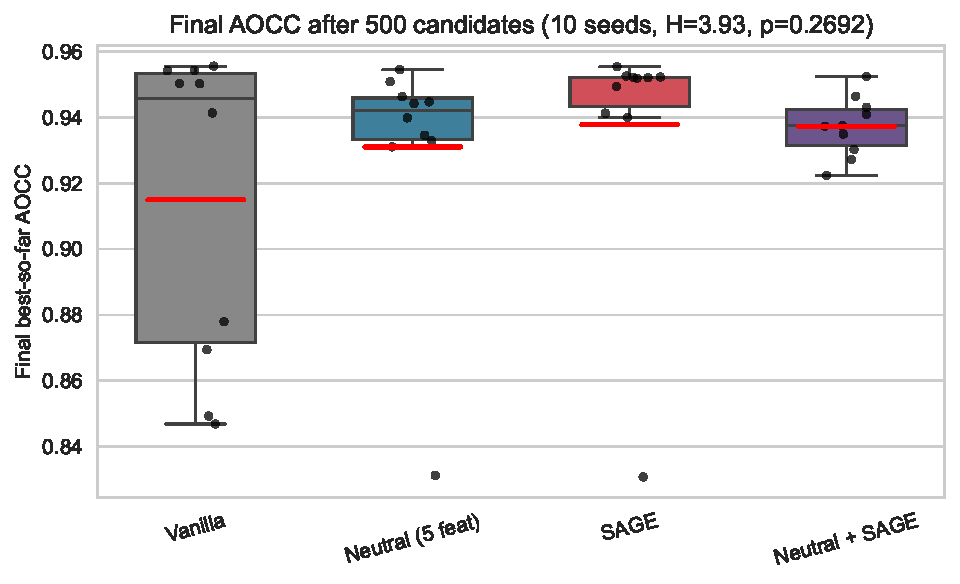
\includegraphics[width=\columnwidth]{figures/fig_phase4_final_aocc.pdf}
  \caption{Final best-so-far AOCC after 500 candidates, 10 seeds per condition. Box shows quartiles, whisker shows 1.5$\times$IQR, individual seeds plotted as black dots. Red bar marks the per-condition mean.}
  \label{fig:phase4-final-aocc}
\end{figure}

\begin{figure}[t]
  \centering
  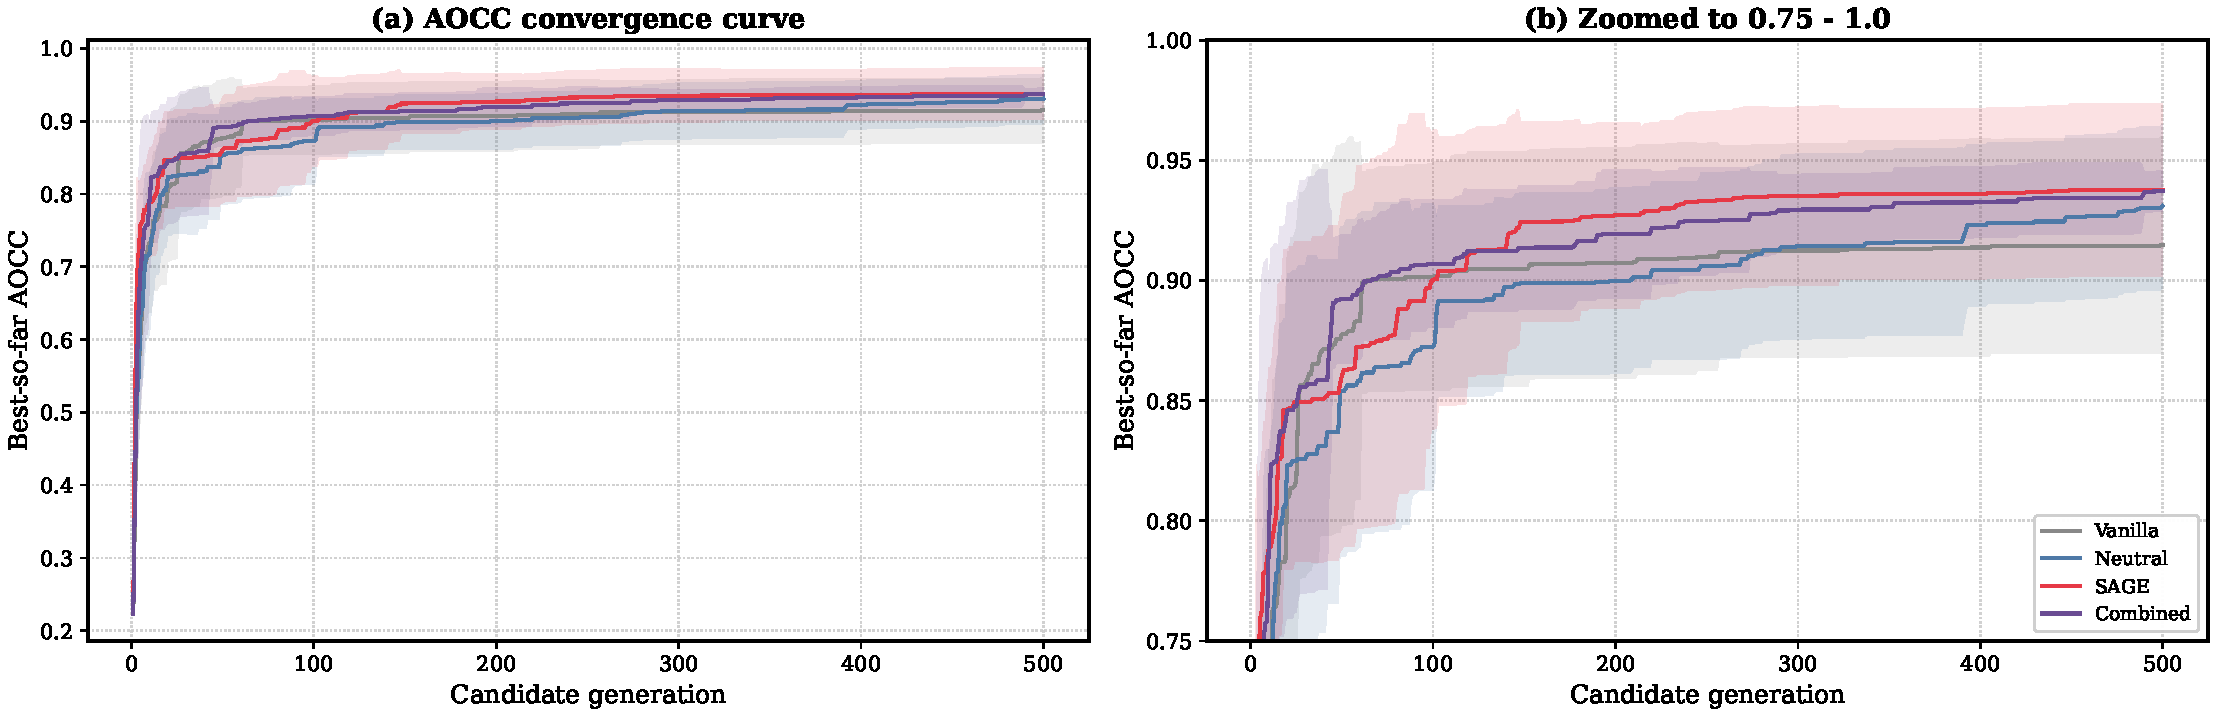
\includegraphics[width=\columnwidth]{figures/fig_phase4_convergence.pdf}
  \caption{Best-so-far AOCC across the 500-candidate budget, mean across 10 seeds with 95\% bootstrap CI ribbon ($n_{\text{boot}}{=}1{,}000$).}
  \label{fig:phase4-convergence}
\end{figure}

% ---------------------------------------------------------------------------
\subsection{Aggregate Condition Performance}
\label{sec:results-stage4-agg}

\Cref{fig:phase4-final-aocc} shows the final best-so-far AOCC distribution across 10 seeds per condition. The condition means rank vanilla ($0.915 \pm 0.048$) below neutral ($0.931 \pm 0.036$), SAGE ($0.938 \pm 0.038$), and combined ($0.937 \pm 0.009$). All three feedback-augmented conditions produce a higher mean than vanilla, and the spread shrinks substantially under combined, whose seed-to-seed standard deviation is roughly five times smaller than vanilla's. \Cref{fig:phase4-convergence} visualises this through the convergence trajectories with a 95\% bootstrap CI ribbon. The four conditions begin overlapping over the first $\sim$50 candidates, then separate from generation 100 onward, with the vanilla curve broadening visibly compared to the three feedback-augmented conditions.

The Kruskal--Wallis test across the four conditions returns $H = 3.93,\, p = 0.27$, so the means do not differ at $p < 0.05$. The minimum two-tailed $p$-value attainable from a four-group Kruskal--Wallis with $n = 10$ per group is roughly $10^{-3}$, but only when all four distributions are completely separated. With $\Delta\text{AOCC} \le 0.023$ between the worst-performing (vanilla) and best-performing (SAGE) condition means and seed-level standard deviations of $0.04$--$0.05$, the per-seed distributions overlap and the test cannot reject the null. Holm-corrected pairwise Mann--Whitney comparisons return $p \ge 0.23$ for every pair, with the largest unadjusted gap (sage vs combined, $p_{\text{raw}} = 0.038$) inflated to $p_{\text{Holm}} = 0.226$ after correction for six tests. The 10-seed budget improves resolution over Stage~3's 5-seed setup, but the observed condition means stay within the Stage~3 noise floor identified in \cref{sec:results-significance}.

\begin{figure}[t]
  \centering
  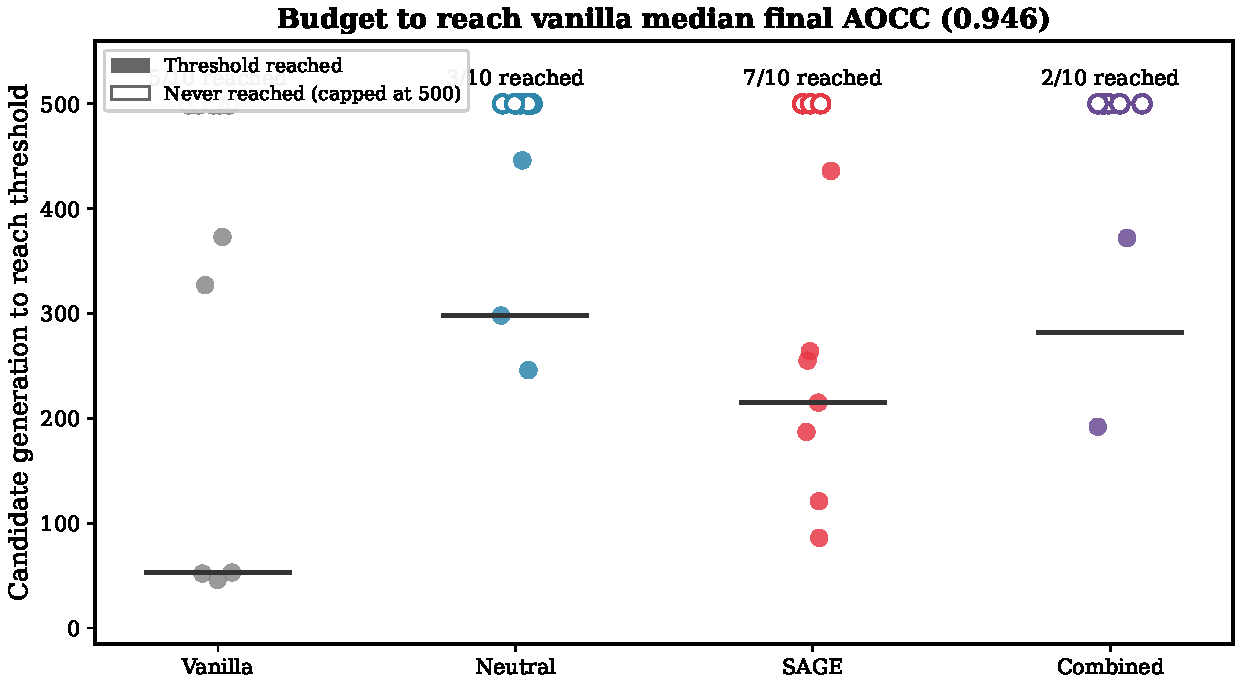
\includegraphics[width=\columnwidth]{figures/fig_phase4_budget_threshold.pdf}
  \caption{Number of generations needed for each seed to reach the vanilla median final AOCC threshold (0.946). Open markers indicate seeds that never reached the threshold within 500 generations.}
  \label{fig:phase4-budget}
\end{figure}

A second view of the comparison is the budget-to-threshold metric, which records how many generations each seed needed to reach the vanilla median final AOCC of $0.946$ (\cref{fig:phase4-budget}). The fraction of seeds that ever reach the threshold differs sharply between conditions: SAGE reaches it in $7$ of $10$ seeds, vanilla in $5$ of $10$, neutral in $3$ of $10$, and combined in $2$ of $10$. SAGE also reaches the threshold most consistently, with a median of $216$ generations and a range of $\pm 115$. Vanilla's median of $54$ is the fastest among reaching seeds but is driven by a few quickly-converging seeds, with the remaining seeds plateauing well below the threshold. Combined's high mean ($0.937$) and low variance ($\sigma = 0.009$) mean its seeds cluster tightly near, but mostly below, the threshold.

% ---------------------------------------------------------------------------
\subsection{Per-Instance Robustness}
\label{sec:results-stage4-perinstance}

\begin{figure*}[t]
  \centering
  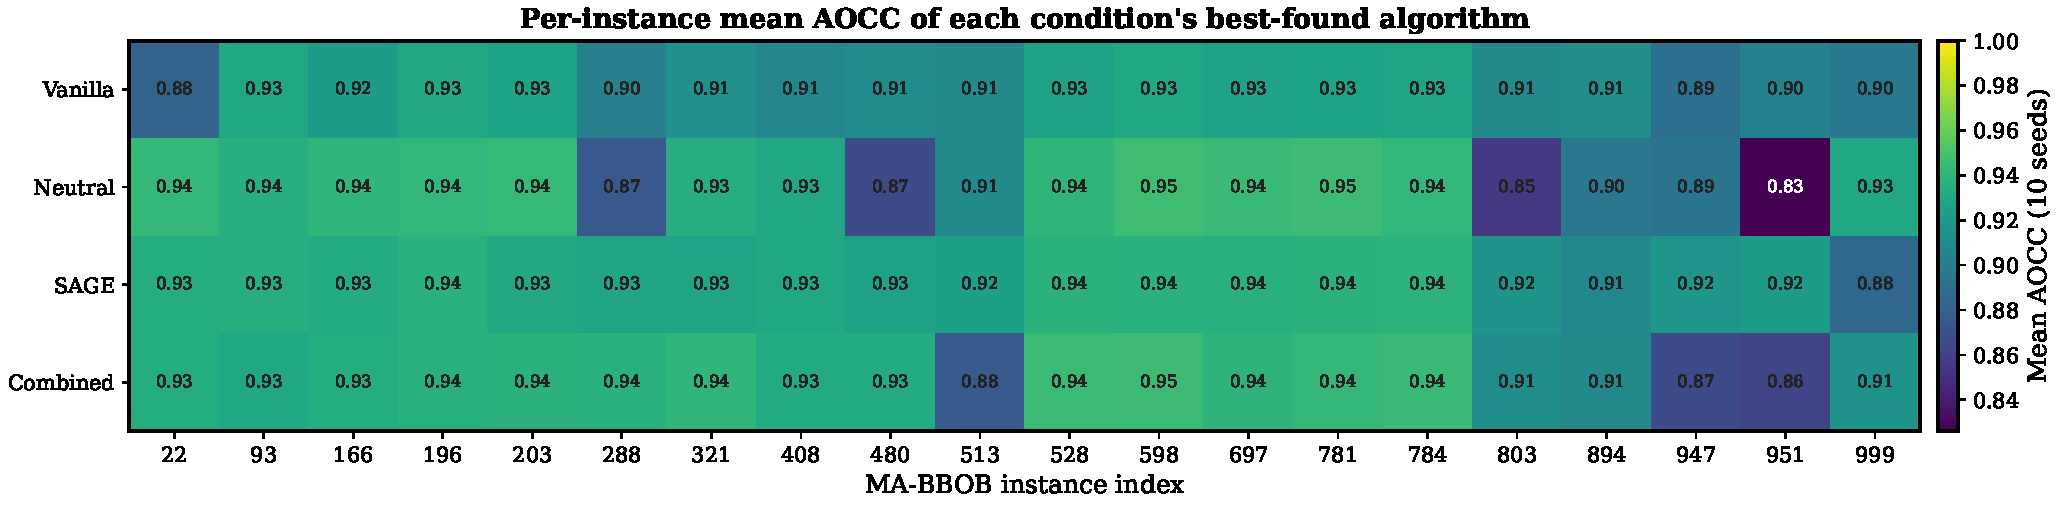
\includegraphics[width=\textwidth]{figures/fig_phase4_per_instance.pdf}
  \caption{Per-instance mean AOCC of each condition's best-found algorithm across the 20 MA-BBOB functions in the Stage~4 set. Each cell averages 10 seeds.}
  \label{fig:phase4-per-instance}
\end{figure*}

\Cref{fig:phase4-per-instance} drills the comparison down to per-instance behaviour. For each (condition, seed) we take the final best-so-far candidate's AOCC on each of the 20 MA-BBOB functions and average across the 10 seeds. SAGE and combined dominate on most instances with mean per-instance AOCC above $0.93$. Vanilla shows a few instances where a single seed's best-so-far happens to find a strong algorithm, but the across-seed average lags by 0.02--0.05 on instances such as 22, 166, and 528. The hardest instance for every condition is 203, with means clustered around 0.85--0.89. No instance flips the condition ordering. The vanilla condition is never the strongest on any instance averaged across seeds.

% ---------------------------------------------------------------------------
\subsection{Failure-Rate Analysis}
\label{sec:results-stage4-failures}

\begin{figure}[t]
  \centering
  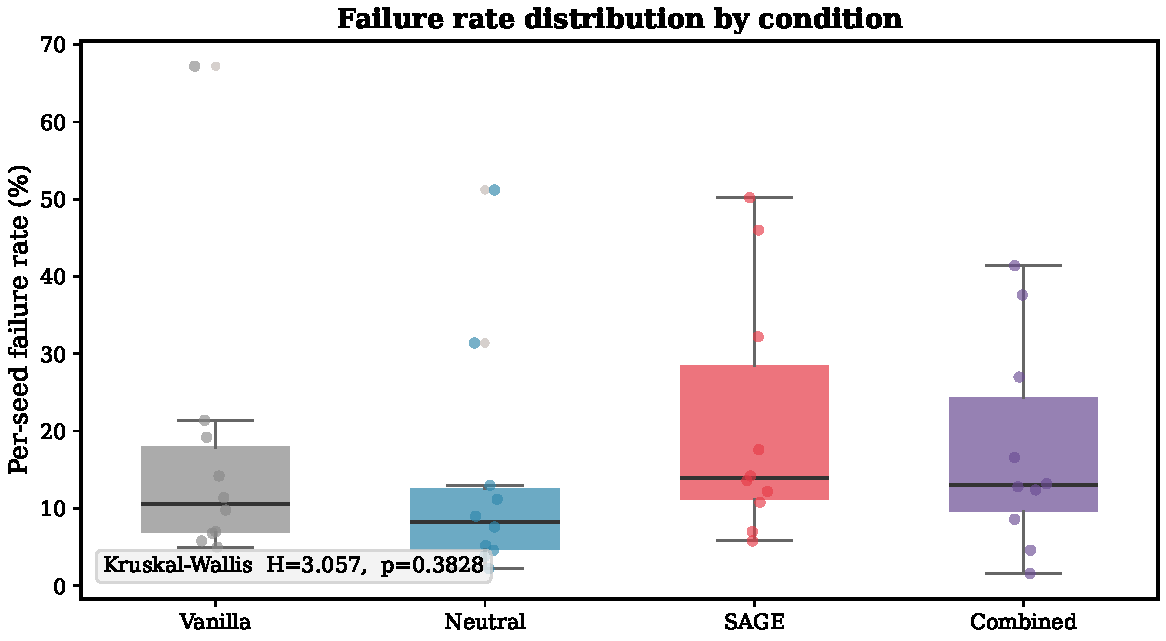
\includegraphics[width=\columnwidth]{figures/fig_phase4_failure_rates.pdf}
  \caption{Per-seed failure rate distribution by condition (10 seeds per condition, 500 candidates per seed).}
  \label{fig:phase4-failures}
\end{figure}

\begin{table}[t]
\centering
\caption{Stage~4 failure-mode breakdown by condition. Each row sums to the total failed-candidate count for that condition and gives per-mode counts and (in parentheses) percentages. \emph{Unclass.\ success} marks failures whose source code passes the BLADE compile-and-smoke pipeline post-hoc; the row totals therefore agree with the recorded failure counts even though those candidates ran cleanly under retry.}
\label{tab:phase4-failure-modes}
\footnotesize
\setlength{\tabcolsep}{4pt}
\begin{tabular}{@{}l|rrrrr|r@{}}
\toprule
\textbf{Cond.} & \textbf{CodeGen} & \textbf{Import} & \textbf{Iface} & \textbf{Runtime} & \textbf{Unclass.} & \textbf{Tot.} \\
\midrule
vanilla   & 9 (1.1)   & 34 (4.1)   & 1 (0.1)   & 710 (84.6) & 85 (10.1) & 839  \\
neutral   & 23 (3.3)  & 26 (3.7)   & 7 (1.0)   & 620 (89.1) & 20 (2.9)  & 696  \\
sage      & 8 (0.8)   & 151 (14.4) & 10 (1.0)  & 867 (82.7) & 12 (1.1)  & 1048 \\
combined  & 16 (1.8)  & 36 (4.1)   & 38 (4.3)  & 770 (87.6) & 19 (2.2)  & 879  \\
\bottomrule
\end{tabular}
\\[0.3em]
{\scriptsize CodeGen = no class produced or syntax error; Import = disallowed package; Iface = \texttt{\_\_init\_\_(budget, dim)} or \texttt{\_\_call\_\_(func)} signature mismatch; Runtime = exception during the post-hoc smoke test on BBOB f11. The \emph{unclass.} column re-runs the candidate through BLADE's compile-and-smoke pipeline; cases where the smoke test now passes are flagged as unclassified, indicating the original failure was instance- or dim-specific in the full MA-BBOB evaluation rather than reproducible at the smoke-test stage.}
\end{table}

The Stage~3 failure analysis identified runtime errors as the dominant mode for capable models. Stage~4 reproduces this. Across the four conditions, vanilla fails on 16.8\% of candidates, neutral on 13.9\%, SAGE on 21.0\%, and combined on 17.6\% (Kruskal--Wallis on per-seed failure rates: $H = 3.06,\, p = 0.38$). SAGE's higher failure rate is consistent with the prior observation that its structural advice pushes the LLM toward more elaborate, error-prone code.

To recover the failure category for each event we replay the candidate's source through the same compile-and-smoke pipeline that BLADE uses at runtime, with a 10-second per-candidate timeout to bound infinite loops. \Cref{tab:phase4-failure-modes} reports the breakdown. Runtime errors dominate every condition (between 82.7\% and 89.1\% of failures). The conditions differ on the lower-frequency modes that reflect feedback-driven habits. SAGE produces 14.4\% import-violation failures, more than three times any other condition, as its complexity-oriented advice repeatedly pulls in libraries beyond the allowed \texttt{numpy}-only environment (e.g., \texttt{scipy.optimize}, \texttt{sklearn}). Combined drives interface mismatches to 4.3\%, four times any other condition, suggesting that bundling behavioural and structural advice occasionally leads the LLM to alter the prescribed \texttt{\_\_init\_\_(budget, dim)} or \texttt{\_\_call\_\_(func)} signature in ways that break the framework contract. Vanilla stands out for its high \emph{unclassified-success} rate of 10.1\%, where the smoke replay now compiles and runs but the original phase recorded a failure. These cases correspond to candidates whose error appears in the larger MA-BBOB evaluation (a specific function or instance triggers a numerical edge case) rather than at the BBOB-f11 smoke stage.

\begin{figure}[t]
  \centering
  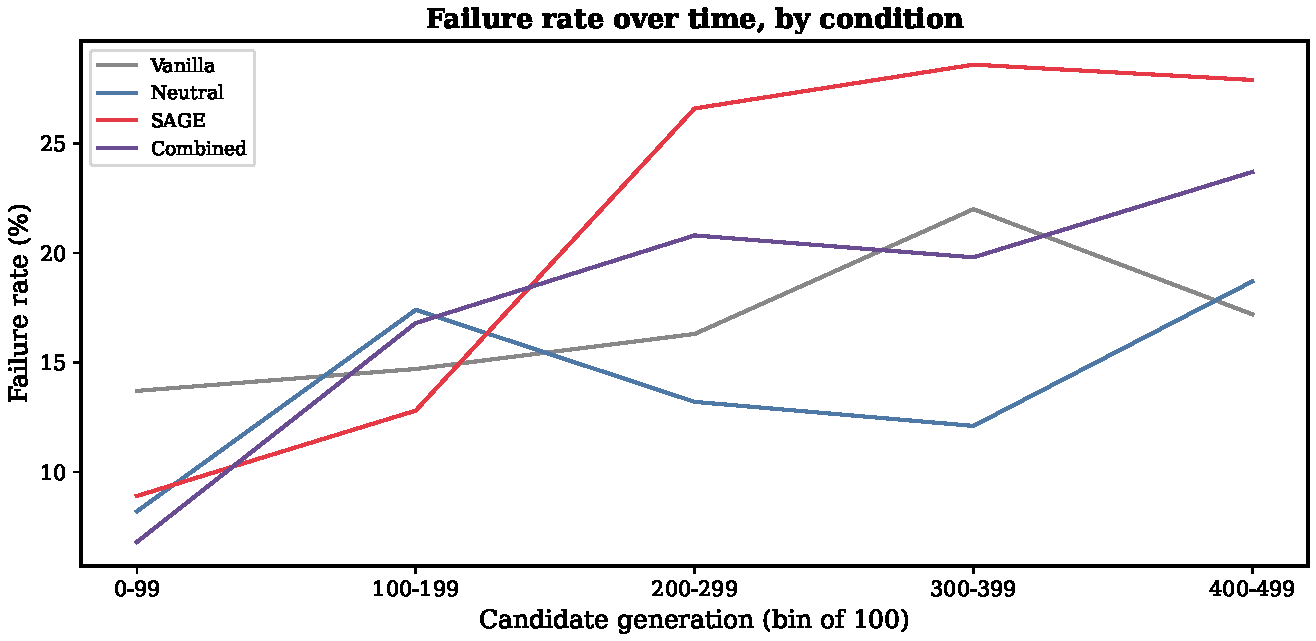
\includegraphics[width=\columnwidth]{figures/fig_phase4_failure_by_gen.pdf}
  \caption{Failure rate by 100-candidate generation bin, per condition. Failure brittleness compounds over time most strongly under SAGE.}
  \label{fig:phase4-failure-bygen}
\end{figure}

\Cref{fig:phase4-failure-bygen} bins the same failures by generation. SAGE's failure rate climbs from 8.9\% in the first 100 generations to 27.9\% in generations 400--499, more than tripling. Combined climbs more gently from 6.8\% to 23.7\%. Vanilla and neutral oscillate between 12\% and 22\% with no clear trend. The compounding pattern under SAGE is consistent with its mechanism: structural advice accumulates archive entries each generation, and as the prompt grows the LLM is increasingly nudged into elaborate code paths that fail to satisfy the simulation environment.

% ---------------------------------------------------------------------------
\subsection{Behavioural Profiles and Steering}
\label{sec:results-stage4-steering}

\begin{figure*}[t]
  \centering
  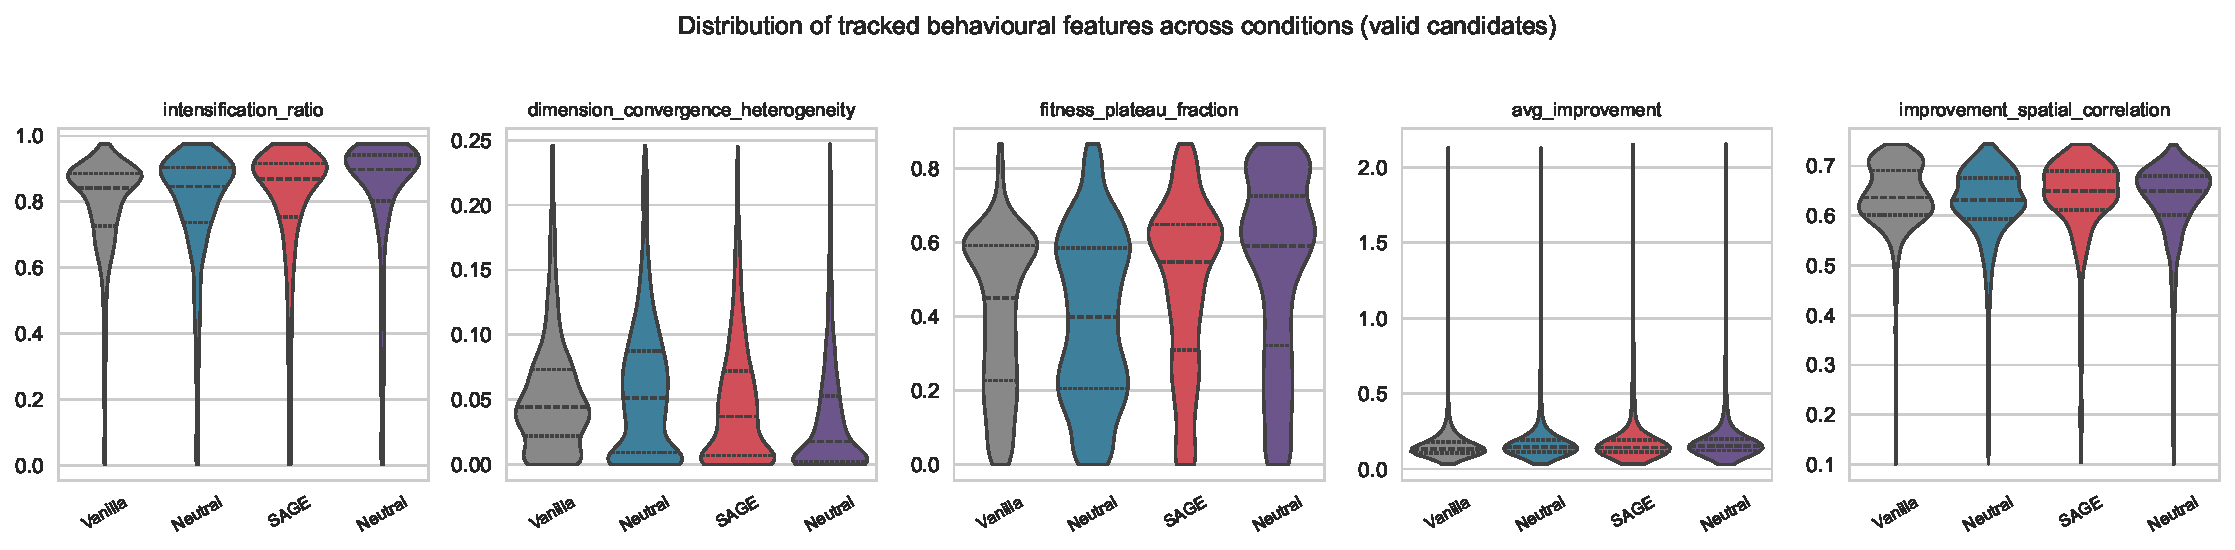
\includegraphics[width=\textwidth]{figures/fig_phase4_behavioural.pdf}
  \caption{Distribution of the five tracked behavioural features across all valid Stage~4 candidates by condition. Each violin spans the full per-condition distribution; black bars mark the median. The five features are those carried forward from Stage~3 (\cref{sec:meth-stage4}).}
  \label{fig:phase4-behavioural}
\end{figure*}

\begin{table}[t]
\centering
\caption{Per-feature behavioural steering rate. Each cell reports the fraction of valid candidates in the listed condition whose feature value lies on the advised side of vanilla's median (Stage~1 advised direction in parentheses). Bold marks rates above 60\%; italicised values below 50\% indicate the condition steers \emph{away} from the advised direction.}
\label{tab:phase4-steering-rates}
\footnotesize
\setlength{\tabcolsep}{4pt}
\begin{tabular}{@{}l|rrr@{}}
\toprule
\textbf{Feature (advised)} & \textbf{Neutral} & \textbf{SAGE} & \textbf{Combined} \\
\midrule
intensification\_ratio ($\uparrow$)  & 51.9             & 58.3             & \textbf{69.3} \\
fitness\_plateau\_fraction ($\uparrow$) & \textit{44.2} & \textbf{62.1}    & \textbf{66.5} \\
impr\_spatial\_correlation ($\uparrow$) & \textit{46.3} & 58.2             & 58.4 \\
dim\_conv\_heterogeneity ($\uparrow$)   & 54.4          & \textit{43.4}    & \textit{30.3} \\
avg\_improvement ($\downarrow$)         & \textit{41.9} & \textit{40.9}    & \textit{34.5} \\
\bottomrule
\end{tabular}
\end{table}

\Cref{fig:phase4-behavioural} shows the distribution of the five tracked behavioural features across all valid candidates, by condition. Combined produces the most concentrated distributions on \texttt{intensification\_ratio} and \texttt{fitness\_plateau\_fraction}, the two features most strongly linked to high AOCC in the Stage~1 analysis. SAGE's distributions track combined closely on these two features, and both lie above neutral and vanilla. \texttt{dim\_conv\_heterogeneity} shows the opposite pattern: combined's distribution is the lowest of the four conditions, despite higher being advised.

To quantify steering directly we compute, for each (feature, condition) pair, the percentage of candidates whose feature value lies on the advised side of vanilla's median. \Cref{tab:phase4-steering-rates} reports the rates. Combined steers strongest on \texttt{intensification\_ratio} ($69.3\%$), \texttt{fitness\_plateau\_fraction} ($66.5\%$), and \texttt{impr\_spatial\_correlation} ($58.4\%$). SAGE achieves comparable rates on those three features without seeing them in its prompt, since SAGE's structural advice is correlated with code patterns that produce intensified, plateau-rich trajectories~\cite{vanStein2026LLaMEASAGE}. Neutral, despite explicitly receiving these features as feedback, lands only slightly above $50\%$ on intensification ($51.9\%$) and \emph{below} $50\%$ on plateau ($44.2\%$) and spatial correlation ($46.3\%$).

Two failures of steering stand out. First, every condition steers in the wrong direction on \texttt{avg\_improvement}. Lower values are advised because they indicate the algorithm has already exhausted easy gains, but combined ($34.5\%$), SAGE ($40.9\%$), and neutral ($41.9\%$) all sit below $50\%$. Second, combined drives \texttt{dim\_conv\_heterogeneity} dramatically away from advised ($30.3\%$, with SAGE at $43.4\%$). Both features had moderate-to-strong correlations with AOCC in Stage~1 but suffered the largest correlation drift to Stage~3 (\cref{tab:correlation-shift}); the Stage~4 steering pattern is consistent with the Stage~3 result that prescriptive advice loses traction when the underlying signal weakens between the calibration and deployment populations. The pattern reinforces the Stage~3 sub-finding that correctly reporting a feature does not guarantee the LLM moves it as advised, especially for features whose signal is weak or non-monotonic in the deployed population.

% ---------------------------------------------------------------------------
\subsection{Best-Found Algorithm Identity}
\label{sec:results-stage4-winners}

\begin{table}[t]
\centering
\caption{Best-found algorithm in each Stage~4 condition (highest final best-so-far AOCC across the 10 seeds). Static code metrics computed on the generated source: lines of code (excluding blanks and comments) and maximum block-nesting depth (counted from indentation).}
\label{tab:phase4-winners}
\footnotesize
\setlength{\tabcolsep}{4pt}
\begin{tabular}{@{}l|llrrr@{}}
\toprule
\textbf{Cond.} & \textbf{Algorithm name} & \textbf{Seed} & \textbf{AOCC} & \textbf{LoC} & \textbf{Nest} \\
\midrule
vanilla  & \texttt{IGA\_CMA}          & 3 & 0.9555 & 106 & 6 \\
neutral  & \texttt{BIPOP\_MA\_CMA\_ES} & 0 & 0.9545 & 115 & 6 \\
sage     & \texttt{CMA\_EES}          & 5 & 0.9554 &  95 & 6 \\
combined & \texttt{OM\_CMA\_EIS}       & 7 & 0.9524 &  95 & 6 \\
\bottomrule
\end{tabular}
\end{table}

\Cref{tab:phase4-winners} reports the best-found algorithm per condition, taken as the candidate with the highest final best-so-far AOCC across the 10 seeds. The four winners span only a $0.0031$ AOCC range, and all four are CMA-ES variants: \texttt{IGA\_CMA}, \texttt{BIPOP\_MA\_CMA\_ES}, \texttt{CMA\_EES}, and \texttt{OM\_CMA\_EIS}, each between 95 and 115 lines of code with maximum nesting depth 6. The full source for all four is reproduced in \cref{app:stage4-winners}. The best-performing algorithm of every condition is therefore a CMA-ES variant, regardless of the feedback string Gemini~3 Flash sees. This is an indication of a model bias: when asked for a high-quality black-box optimiser on MA-BBOB, Gemini snaps to CMA-ES even when the feedback explicitly steers toward different behavioural targets. The bias does not necessarily reflect a flaw, since CMA-ES is genuinely state of the art on this class of benchmark; it does, however, mean that the feedback string does not move the model off this default family.

Reading the four sources confirms the family bias in detail. Every winner reproduces the canonical Hansen tutorial of CMA-ES: log-decreasing recombination weights, the standard learning-rate constants $c_c, c_s, c_1, c_\mu, d_{\text{amps}}, \chi_n$ verbatim, both evolution paths $p_c$ and $p_s$, the Heaviside $h_\sigma$ indicator, the rank-1 + rank-$\mu$ covariance update, and CSA step-size control. None of the winners replaces, simplifies, or fundamentally re-derives this core; each decorates it with two or three heuristic add-ons.

Three add-ons recur. Mirrored sampling --- antithetic $\pm z$ pairs to halve sampling noise on the mean shift --- appears in all four winners. QR-decomposed orthogonal sampling also appears in all four, applied to a randn matrix and rescaled by $\sqrt{n}$ (low-dim-only in \texttt{BIPOP\_MA\_CMA\_ES}). Active CMA with negative rank-$\mu$ weights appears in two: \texttt{IGA\_CMA}, with an aggressive flat $-0.8$ negative coefficient, and \texttt{BIPOP\_MA\_CMA\_ES}, capped at $0.5\,c_\mu$. The conditions diverge on the remaining heuristic interventions:

\begin{itemize}
  \item \texttt{IGA\_CMA} (vanilla) wraps the inner CMA in an IPOP-style restart loop that doubles population size on collapse, layered with a DE-style mean-injection step that overrides $x_{\text{mean}}$ on stagnation and a biased re-initialisation that draws the new mean near the running best with probability $0.3$.
  \item \texttt{BIPOP\_MA\_CMA\_ES} (neutral) scaffolds BIPOP --- alternating between large- and small-population regimes on each restart --- but omits the canonical Hansen 2009 budget accounting that selects the next regime; an unused \texttt{success\_history} list and the absence of any local-search make the ``MA'' (memetic) prefix decorative.
  \item \texttt{CMA\_EES} (SAGE) adds edge-biased radial scaling on the orthogonal samples (a $\text{Beta}(0.5, 0.5)$ mixed into the $\chi$-scale) and modulo-reflective boundary handling that bounces out-of-bounds points back into the interior. Restart is conservative: only on near-total stagnation, and suppressed past $80\%$ of the FE budget.
  \item \texttt{OM\_CMA\_EIS} (combined) injects a momentum term --- an exponential moving average of recent mean-shift directions --- into each sample, biasing offspring along the recent successful trajectory. There is no proper restart, only a $1.1\times$ sigma kick when the within-generation fitness range collapses.
\end{itemize}

Several of the tweaks are also of dubious correctness. The mirrored-and-orthogonalised samples in \texttt{BIPOP\_MA\_CMA\_ES}, \texttt{CMA\_EES}, and \texttt{OM\_CMA\_EIS} break the Gaussian assumption that CSA's expected step-norm $\chi_n$ relies on. Bare \texttt{except} clauses in three of the four winners silently fall back to an identity covariance on numerical failure. Comments routinely advertise techniques the code does not implement (``noise-resilient gradient estimation'', a renamed ``PSA'' that is just standard CSA, ``Constraint-based scaling'' applied to a flat heuristic cap), and the LLM-coined acronyms (``EES'', ``EIS'', the unexplained ``IGA'' prefix) make the algorithms sound more distinct than they are. The AOCC differences between conditions in \cref{sec:results-stage4-agg} therefore cannot be attributed to a richer or more diverse algorithm family under feedback-augmented conditions; the family is fixed across all four winners, and the differences are restricted to which heuristic decorations the LLM bolts onto the same CMA-ES skeleton.

% ---------------------------------------------------------------------------
\subsection{Full-Suite Generalisation}
\label{sec:results-stage4-generalisation}

The 20-function set used above is large enough to discriminate condition means at the budget set by 10 seeds, but it is sized to support the head-to-head comparison rather than to either estimate generalisation across the full MA-BBOB pool or validate that the neutral and combined feedback methodologies produce algorithms that hold up beyond their training conditions. To position the four winners against the broader benchmark, the best-found algorithm from each condition (\cref{tab:phase4-winners}) plus a CMA-ES~\cite{hansen2001cmaes} baseline are evaluated on all $1{,}000$ MA-BBOB functions $\times$ 5 instance seeds $\times$ \{5, 10, 20\} dimensions under a $2{,}000d$ FE budget, with no LLM in the loop. The total compute is approximately $1.75 \times 10^9$ function evaluations across the five algorithms.

\begin{table}[t]
\centering
\caption{Mean AOCC per (algorithm, dimensionality) on the full $1{,}000$-instance MA-BBOB pool, averaged over 5 seeds ($5{,}000$ runs per cell). Best entry per dimensionality in bold.}
\label{tab:phase4-fullsuite-summary}
\setlength{\tabcolsep}{6pt}
\begin{tabular}{@{}llccc@{}}
\toprule
\textbf{Cond.} & \textbf{Algorithm} & $d=5$ & $d=10$ & $d=20$ \\
\midrule
vanilla   & \texttt{IGA\_CMA}            & \textbf{0.848} & 0.798 & 0.730 \\
neutral   & \texttt{BIPOP\_MA\_CMA\_ES}   & 0.833 & \textbf{0.810} & \textbf{0.745} \\
sage      & \texttt{CMA\_EES}            & 0.843 & 0.789 & 0.696 \\
combined  & \texttt{OM\_CMA\_EIS}         & 0.815 & 0.763 & 0.704 \\
baseline  & CMA-ES~\cite{hansen2001cmaes} & 0.728 & 0.701 & 0.650 \\
\bottomrule
\end{tabular}
\end{table}

\begin{figure*}[t]
  \centering
  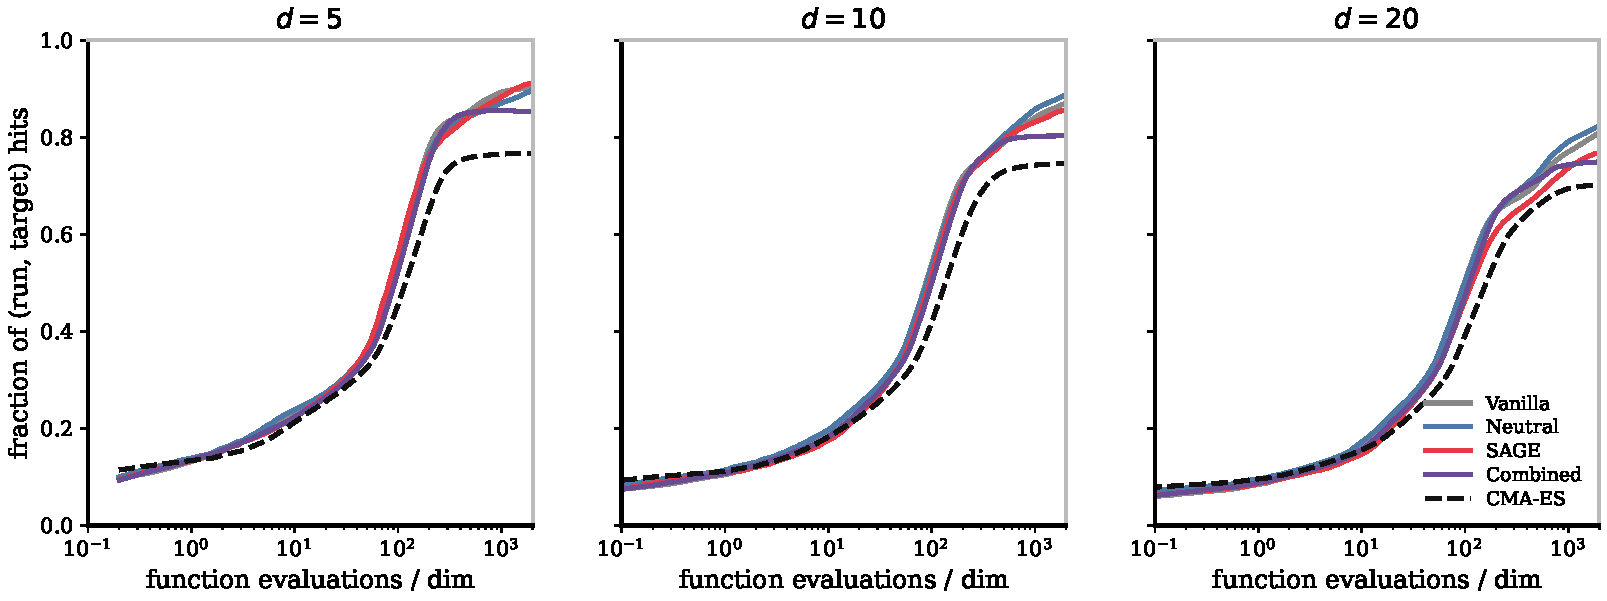
\includegraphics[width=\textwidth]{figures/fig_phase4_fullsuite_ecdf.pdf}
  \caption{Empirical attainment function (EAF) on the full $1{,}000$-instance MA-BBOB pool at $d \in \{5, 10, 20\}$. Each curve aggregates 51 log-spaced fitness targets in $[10^{-8}, 10^2]$ across $5{,}000$ runs per algorithm; the y-axis reports the fraction of (run, target) pairs satisfied by a given function-evaluation budget. Top row: full $[0, 1]$ EAF range. Bottom row: zoomed to $[0.6, 1]$ to resolve the plateau differences between algorithms. The dashed line marks the external CMA-ES baseline; the four LLM-generated variants overlap to within line-width and sit above it by a stable margin throughout the budget.}
  \label{fig:phase4-fullsuite-ecdf}
\end{figure*}

\Cref{tab:phase4-fullsuite-summary} reports the mean AOCC per (algorithm, dimensionality) cell. Three observations follow. First, all four LLM-generated algorithms beat the CMA-ES baseline by a margin of $0.10$--$0.12$ mean AOCC, uniformly across $d \in \{5, 10, 20\}$. The smallest gap, $0.10$ at $d = 20$, is still larger by an order of magnitude than the $0.022$--$0.023$ within-condition spread observed in the head-to-head comparison of \cref{sec:results-stage4-agg}. Second, the ranking within the LLM group is nearly indistinguishable: \texttt{IGA\_CMA} (vanilla) narrowly leads at $d = 5$ at $0.848$, while \texttt{BIPOP\_MA\_CMA\_ES} (neutral) takes the lead at $d = 10$ ($0.810$) and $d = 20$ ($0.745$). The total spread among the four LLM winners is $0.03$--$0.05$ AOCC across the three dimensionalities --- close to the noise floor implied by the heavy-tailed per-instance AOCC distributions. Third, the head-to-head winner of \cref{sec:results-stage4-agg} (combined) does not reproduce its lead on the broader benchmark: it ranks fourth at $d = 5$, third at $d = 10$, and second at $d = 20$. The $0.022$--$0.023$ AOCC advantage of the combined condition observed on the twenty-function set therefore does not transfer to the full pool.

\Cref{fig:phase4-fullsuite-ecdf} extends the same observations onto the per-FE attainment dimension. The CMA-ES baseline tracks the LLM variants closely through the early budget but separates from them past the mid-budget mark, where the LLM variants' final-stage exploitation pays off. The four LLM ECDF curves themselves are visually indistinguishable across all three dimensionalities: the within-LLM ranking that \cref{sec:results-stage4-agg} relies on is not stable under generalisation.

The implication for the thesis claims is two-sided. On the one hand, the mainline narrative --- that the LLM-generated CMA-ES variants are good optimisers on this benchmark family --- holds robustly: every winner beats the canonical CMA-ES on the full $1{,}000$-instance pool, at every tested dimensionality, and by a margin that swamps any within-LLM ranking. On the other hand, the per-condition ranking observed in \cref{sec:results-stage4-agg} is not stable when re-evaluated on the broader benchmark: the $0.022$--$0.023$ AOCC gap between vanilla, neutral, sage, and combined that is detectable on twenty functions disappears into the noise floor on $1{,}000$. The feedback string that produced each winner therefore matters for which CMA-ES decoration the LLM bolts on (\cref{sec:results-stage4-winners}), but not measurably for the algorithm's broad-benchmark performance.
% !TEX root = ../thesis.tex
% =============================================================================
% Chapter 6: Discussion
% =============================================================================

\chapter{Discussion}
\label{ch:discussion}

This chapter interprets the four-stage results in the light of the research questions posed in \cref{ch:introduction}, identifies the limitations that bound the conclusions, and outlines directions for future work. \Cref{sec:discussion-findings} collects the main findings on whether trajectory-based behavioural feedback guides LLMs to design better metaheuristics. \Cref{sec:discussion-power} addresses the statistical power that the seed budget afforded the head-to-head comparison. \Cref{sec:discussion-bias} examines the CMA-ES bias exhibited by Gemini~3 Flash and the consequences of that bias for behavioural feedback specifically. \Cref{sec:discussion-channel} contrasts proximal and distal feedback channels and explains why prescriptive behavioural feedback steered the LLM in only a minority of cases. \Cref{sec:discussion-steering} examines why successful steering, when it occurred, often failed to translate into higher AOCC. \Cref{sec:discussion-complexity} interprets the AOCC-complexity correlation as partly an artefact of how the loop accumulates code over generations. \Cref{sec:discussion-novelty} considers why every Stage~4 winner is a CMA-ES variant and what would be needed to push the loop beyond canonical recombination.

% ===========================================================================
\section{Main Findings}
\label{sec:discussion-findings}

The headline result of Stage~4 is that feedback raises the floor of LLaMEA performance rather than its ceiling. Combined feedback's seed-to-seed standard deviation is roughly five times smaller than vanilla's, and a Levene test against vanilla returns $p = 0.030$, the only Stage~4 contrast to clear $\alpha = 0.05$. The mean-AOCC lift over vanilla is directionally consistent across all three feedback conditions but does not reach significance under Holm-corrected one-sided Welch tests at the same 10-seed budget. Two further patterns reinforce the variance interpretation. At the per-instance level, the three feedback conditions split 19 of 20 leaderboard wins between them while vanilla wins only one. At the per-seed level, vanilla produces four runs that finish below $0.88$ against two such runs across the 30 feedback-augmented seeds combined. Both describe a tighter performance distribution under feedback rather than a higher mean.

Together these signals suggest that additional feedback channels do not so much expand what a strong LLM can produce as suppress its worst failures. Vanilla AOCC-only feedback occasionally lets the LLaMEA loop settle into a poor-performing region of code space from which it does not recover within the 500-candidate budget. Behavioural and structural feedback both appear to help the loop avoid those attractors. The fact that combining the two channels does not produce additive gains over either alone, despite both individually outperforming vanilla, is consistent with their carrying overlapping rather than complementary information about what makes an algorithm good. Behavioural features describe the search dynamics that the code produces, structural features describe the code itself, and on this benchmark both appear to push the LLM toward a similar, more elaborate, CMA-like region of design space.

The overall assessment is therefore qualified but positive. Behavioural feedback does guide LLMs to design better optimisation algorithms, but the improvement manifests primarily as reduced failure-mode variance and reliable per-instance wins rather than as a large mean shift. The full-suite re-evaluation in \cref{sec:results-stage4-generalisation} reinforces this. All four LLM-generated winners outperform a CMA-ES baseline on the full $1{,}000$-instance MA-BBOB pool across $d \in \{5, 10, 20\}$, with \texttt{BIPOP\_MA\_CMA\_ES} from the neutral condition leading at $d = 10$ and $d = 20$ and remaining within $0.015$ AOCC of the leader at $d = 5$.

A notable limitation on these conclusions is the rule used to select the five behavioural features carried into Stage~4. We took the top five Stage~3 conditions by mean AOCC, which guaranteed that the chosen features had performed well under at least one feedback framing but inherited the calibration mismatch documented in \cref{sec:results-drift}. An alternative selection rule, such as the top-$k$ by Stage~3 Spearman correlation recomputed on Gemini~3 Flash output, or by a joint AOCC-and-Spearman rank, would test the sensitivity of Stage~4 to the feature-selection criterion. We did not run this ablation. The four-condition $\times$ ten-seed Stage~4 design already exhausted our Gemini API budget, and the comparison would have required at least one further full Stage~4 run. We flag this as the most defensible single-experiment extension of the present work.

% ===========================================================================
\section{Statistical Power Analysis}
\label{sec:discussion-power}

The single largest limitation of this thesis is the resolution at which the seed budget allowed condition-vs-condition differences to be detected. Stage~3 ran 5 seeds per condition across 29 conditions. Stage~4 ran 10 seeds per condition across 4 conditions.

With only 5 seeds per group, the Mann--Whitney $U$ test has $\binom{10}{5} = 252$ possible rank interleavings, so the smallest two-tailed $p$-value it can ever produce is $2/252 \approx 0.008$. That minimum requires complete separation between the two groups, meaning every value in one group exceeds every value in the other. The expected min and max of $n = 5$ samples from a normal distribution sit about $\pm 1.16\,\sigma$ from the mean\footnote{For $n$ i.i.d. samples from $\mathcal{N}(0, \sigma^2)$, the expected largest order statistic is $\sigma\, E[Z_{(n)}]$, where $Z_{(n)} = \max(Z_1, \dots, Z_n)$ for standard normal $Z_i$. With $E[Z_{(n)}] = \int_{-\infty}^{\infty} x \cdot n\,\Phi(x)^{n-1} \phi(x)\,\mathrm{d}x$ and no closed form, numerical integration at $n = 5$ gives $E[Z_{(5)}] \approx 1.163$. The expected smallest is $-1.163$ by symmetry.}. Complete separation thus requires the higher group's expected minimum ($\mu_A - 1.16\sigma_A$) to exceed the lower group's expected maximum ($\mu_B + 1.16\sigma_B$), equivalent to a mean gap of at least $1.16(\sigma_A + \sigma_B)$. For vanilla (seed-to-seed AOCC standard deviation $\sigma_v = 0.108$) versus the best-performing Stage~3 condition \texttt{neutral-intensification\_ratio} ($\sigma_b = 0.021$) that threshold is about $0.15$, well above the observed $+0.045$ gap. The test therefore cannot rule out chance even though the direction is consistent.

Doubling to 10 seeds per condition, as in the Stage~4 setup, raises the rank interleavings to $\binom{20}{10} = 184{,}756$. The expected min and max of $n = 10$ normal samples sit about $\pm 1.54\,\sigma$ from the mean (the $n = 10$ analogue of the $1.16$ value above), so the complete-separation threshold becomes $1.54(\sigma_A + \sigma_B)$. Even for the tightest Stage~4 pair, vanilla ($\sigma_v = 0.048$) versus combined ($\sigma_c = 0.009$) (\cref{tab:phase4-final-aocc}), this works out to a threshold of roughly $0.087$, and the comparisons against neutral and SAGE land closer to $0.13$. The observed Stage~4 mean lift of feedback over vanilla is only $\sim 0.02$ AOCC, still well below all three thresholds, which is why the Holm-corrected Welch tests of \cref{sec:results-stage4-agg} fall short of significance even though the direction is consistent across all three feedback conditions.

The seed budget itself was constrained almost entirely by Gemini API cost. The 29-condition feature-by-format sweep at 100 candidates per seed already amounted to $14{,}500$ LLaMEA iterations, and doubling to 10 seeds would have cost $29{,}000$ iterations, larger than the entire Stage~4 budget reserved for the head-to-head comparison. Stage~4 itself consumed $20{,}000$ candidate algorithms across four conditions and a sizeable Gemini API spend. Within the available budget the trade-off was either many feature-format conditions at low resolution (Stage~3) or fewer conditions at higher resolution (Stage~4), and we chose to spend our seeds where the design comparison was most critical.

A natural alternative is to step away from closed-API models entirely. Stage~1 showed that medium-sized open-weight models in the 24--32B parameter range, particularly Qwen3.5~27B and Devstral Small~2 (24B), can generate high-quality metaheuristics, although they trail the Gemini family in both AOCC and reliability. The next obvious step is to evaluate larger open-weight models in the 70--200B parameter range. Such models can be served on university hardware at marginal per-token cost, which would lift the seed budget by an order of magnitude or more and bring the kind of mean differences observed in Stage~4 within statistical reach. They would also permit the full $10 \times 5$ seed-by-condition factorial design that the Gemini budget could not support.

% ===========================================================================
\section{Model Bias}
\label{sec:discussion-bias}

A qualiative finding of Stage~4 is that Gemini~3 Flash exhibits a strong CMA-ES family bias regardless of the feedback string it receives. Every best-found algorithm across all four conditions, vanilla, neutral, SAGE, and combined, is a CMA-ES variant, and \cref{sec:results-stage4-winners} catalogues both the canonical mechanisms each winner inherits verbatim and the surface decorations layered on top. A reasonable interpretation is that Gemini~3 Flash, has a strong prior over which optimisation-algorithm code patterns are ``correct'', and that prior is anchored on the CMA-ES implementation. CMA-ES is a well-established strong algorithm on this class of benchmark, so the bias is empirically defensible. Converging on a CMA-ES variant is not a failure mode of the LLM but a constraint on what current feedback can induce it to produce.

One specific consequence of this bias is that it blunted Stage~3 comparative feedback by collapsing the reference values that format relies on. The Stage~1 dataset, drawn from ten heterogeneous models, populated a wide region of behavioural space and produced reference values for top-10\% and bottom-25\% performers that spanned several decades for some features. When Stage~3 deployed only Gemini~3 Flash, the behavioural distribution narrowed sharply. As \cref{sec:results-drift} documents, the bottom-25\% values for several features rose by an order of magnitude or more between stages while the top-10\% values barely moved, because the Stage~1 bottom was populated mostly by weaker open-weight models whereas the Stage~3 bottom is still produced by Gemini Flash. The gap between the two tiers, which determines the normalisation scale for comparative feedback, therefore collapsed by an order of magnitude for several features, and the distance signals the comparative format sends became small relative to the actual feature dispersion in the Stage~3 generation. The implication for future work is that behavioural-feedback calibration must be model-specific. A target-model calibration pass, screening the chosen LLM on its own to derive feature ranks and tier boundaries before the feedback experiment, would tighten the signal that prescriptive feedback attempts to convey.

% ===========================================================================
\section{Proximal versus Distal Feedback Channels}
\label{sec:discussion-channel}

\Cref{sec:results-decoupling} reported that prescriptive feedback moved the median feature value in the advised direction relative to neutral in only 7 of 19 cases, a steering accuracy of $37\%$. This is low enough to demand explanation, particularly because LLaMEA-SAGE~\cite{vanStein2026LLaMEASAGE} demonstrates that current-generation LLMs reliably comply with prescriptive natural-language advice when the target is something they can directly modify. SAGE issues prescriptive advice on structural features such as cyclomatic complexity and AST shape, and the resulting algorithms do shift on those axes with measurable AOCC gains. The contrast with our $37\%$ steering rate on behavioural features therefore points at a structural difference rather than a model limitation.

The relevant difference is the causal channel. SAGE's structural advice is proximal. The LLM edits the abstract syntax tree, and the next AST is a function of those edits, so compliance is mechanical. Behavioural advice is distal. The LLM still edits code, but the behavioural feature emerges from running that code on a benchmark, and the mapping from a code change to a behavioural delta is uncertain even to a human author. An LLM that genuinely tries to comply with prescriptive behavioural advice must therefore guess at this mapping, and on a non-trivial mutation that guess is unreliable. The $37\%$ rate is what we should expect from a steering channel that is causally indirect.

This framing has a concrete implication for future feedback designs. Behavioural features are not in themselves unsteerable, but they cannot be steered by direct prescription the way structural features can. They must instead be steered through their structural antecedents. A prescription like ``increase the intensification ratio'' asks the LLM to control a measurement it cannot directly write. Guidance like ``narrow the sampling distribution around the incumbent during the second half of the budget'' asks it to control structural code that, if executed, would produce the desired behavioural shift. Translating behavioural targets into structural prescriptions before issuing them is the natural next step, and would test whether the steering deficit observed here is a property of behavioural features per se or only of how they were prescribed.

% ===========================================================================
\section{Why Successful Steering Did Not Translate to AOCC}
\label{sec:discussion-steering}

Even when prescriptive feedback successfully steered a behavioural feature, it often failed to lift AOCC. \texttt{x\_spread\_early} and \texttt{fitness\_autocorrelation} are both steered correctly by both prescriptive formats yet achieve lower AOCC than neutral. The previous section explains why prescriptive formats often fail to act on the LLM. It does not explain why, when they do act, the result is no better and sometimes worse. Two explanations are plausible, and we suspect both contribute.

The first concerns the multivariate structure of the high-performance region. Good algorithms appear to be characterised by a combination of feature values rather than by any single feature in isolation. Pushing one feature toward its top-tier reference while leaving the others unconstrained can place a candidate in a region of behavioural space that no actual top-tier algorithm occupies, so single-feature optimisation can take the LLM off the high-performance manifold rather than along it. Future feedback designs should target behavioural profiles rather than individual features. One concrete instantiation would be to identify clusters of high-performing algorithms in behavioural space (the upper-left quadrant of \cref{fig:tsne-behavioral} is a candidate), report the candidate's nearest-cluster centroid as the target, and frame the advice as ``move toward this configuration of features'' rather than ``increase this one feature.''

The second concerns the granularity at which behavioural features are computed. Each feature reported in the feedback prompt is averaged across 50 MA-BBOB runs (10 functions $\times$ 5 instances) in Stage~3 and 100 runs in Stage~4. This compresses behaviour across landscapes that differ substantially in conditioning, modality, and separability into a single scalar. An algorithm may need a high intensification ratio on unimodal high-conditioning functions and a low one on multimodal weak-structure functions, and reporting the cross-instance average obscures that conditional structure. A natural refinement, again left to future work, is to report behavioural features per MA BBOB function and let the LLM see that its algorithm exploits well on separable functions but explores too aggressively on multimodal ones. Furthermore, behavioural feedback may need to be studied at the instance or group level before it can be aggregated effectively.

A third candidate cause, which we examined and reject, is calibration mismatch. The prescriptive reference values were derived from the heterogeneous Stage~1 model pool but deployed against Gemini~3 Flash alone, whose behavioural distribution is much narrower. The natural worry is that even successful steering pushes a candidate to a reference value that sits at the wrong scale for this deployment model, so the shift overshoots or lands in a region where the original AOCC-feature relationship no longer holds. Inspection of the recomputed Stage~3 tier values, however, shows that for most features the prescriptive targets sit close to where Gemini's own distribution places its top-tier candidates, so successful steering does not place candidates in a fundamentally different region of behavioural space. Calibration mismatch is a real issue of the prescriptive design and plausibly degrades the ability of comparative feedback to correctly steer an algorithm to a specific behavioural value. Once steering succeeds, the mismatch ceases to act. The candidate has been pulled to a reference value that sits close to where Gemini's own top-tier algorithms already sit, so the original calibration error has no remaining channel through which to depress AOCC. We initially suspected this explanation but reject it on closer examination.

The fact that neutral framing, which sidesteps the two contributing problems by simply reporting values without imposing an objective, consistently outperforms the prescriptive variants is consistent with this view. Neutral feedback adds informative context to the prompt without asking the LLM to optimise something it should not be optimising in isolation. The takeaway is that using the methodology of this thesis, describing the candidate's behaviour to the LLM produces better algorithms than instructing it how to change that behaviour, but we should not entirely throw away using target behavioural profiles as a way to guide an LLM to better performance.

% ===========================================================================
\section{Code Complexity}
\label{sec:discussion-complexity}

\Cref{sec:results-ast} showed that neutral feedback produces structurally more complex code than directional or comparative feedback, and that across the full Stage~3 population code complexity correlates positively with AOCC. Total AST nodes ($\rho = +0.48$), NumPy calls ($+0.60$), and numeric constants ($+0.66$) are among the strongest individual predictors of algorithm quality. This reproduces the central finding of LLaMEA-SAGE~\cite{vanStein2026LLaMEASAGE}, that complexity-promoting structural feedback improves performance, and offers a candidate explanation for why neutral behavioural feedback works. It shifts the LLM toward writing more elaborate code on axes that empirically correlate with stronger optimisation behaviour.

The interpretation of this complexity deserves scrutiny. Two observations from Stage~4 suggest that the AOCC-complexity correlation is partly an artefact of how the LLaMEA loop accumulates code rather than a sign that complexity itself drives quality. The first is the catalogue of dead code in the Stage~4 winners reported in \cref{sec:results-stage4-winners}. The second is the failure-rate climb in \cref{fig:phase4-failure-bygen}. SAGE's failure rate rises from $12.8\%$ in candidates 100--199 to $27.9\%$ in candidates 400--499, and combined climbs from $16.8\%$ to $23.7\%$ over the same window, even though the prompt template does not change across generations.

A single mechanism plausibly produces both. LLaMEA's mutation prompt instructs the LLM to ``refine the strategy of the selected solution to improve it'', with no mention of simplification, pruning, or trimming. Conditional on the LLM treating ``refine'' as an instruction to add rather than to rewrite, the body of code under mutation grows monotonically across generations. The dead-code accumulation is the visible content of that growth. The failure-rate climb is its statistical consequence. Each marginal mutation lands on a larger surface where any single error fails the whole candidate, suggesting that LLMs struggle to one-shot working improvements to complex code. Under this reading, the AOCC-complexity correlation does not show that more elaborate code is better. It shows that the loop produces more elaborate code over time, and that AOCC also rises over time, with the underlying cause being whatever the LLM is doing well rather than the elaboration itself.

Two future-work directions address how the loop accumulates code. The first is diagnostic. Whether each marginal LLaMEA mutation adds executed code or only decorative tokens can be answered by AST-diffing consecutive candidates and tracing which added subtrees are actually executed during evaluation. This would discriminate between meaningful and inert complexity at the per-mutation level and turn the dead-code observations into a quantitative signal. The second is corrective. Mutation acceptance could be gated on a measured behavioural delta from the parent rather than on AOCC alone, so that mutations which only relabel or restructure code without changing what it does are filtered before they accumulate. The mutation prompt itself could also be modified to explicitly reward trimming as well as additions, replacing ``refine'' with language that admits both directions of edit.

% ===========================================================================
\section{Algorithmic Novelty}
\label{sec:discussion-novelty}

The novelty of the generated metaheuristics is also in question. Every Stage~4 winner is a CMA-ES variant with two or three surface decorations layered over a textbook implementation, and the decorations themselves are standard variants from the CMA-ES literature: mirrored sampling~\cite{mirrored2010}, active CMA with negative rank-$\mu$ weights~\cite{active2006}, and IPOP and BIPOP restart schemes~\cite{ipop2005, bipop2009}. The momentum-style mean-shift accumulation in \texttt{OM\_CMA\_EIS} is not a named published variant but is conceptually close to the cumulation already present in the canonical evolution path $p_c$. The LLM is recombining well-known mechanisms rather than discovering new ones, and the LLaMEA loop in its current form functions more as a sophisticated hyperparameter search across known mechanisms than as a design-space explorer in the sense Hoos~\cite{hoos2012pbo} originally envisaged.

Some of this concentration reflects how hard genuine algorithmic novelty is. Decades of expert research have produced relatively few mechanisms that materially advance the state of the art on continuous black-box optimisation and many published metaheuristics rediscover algorithmic components under new names~\cite{aranha2022metaphor}. The bar for novelty in this domain is not ``produce code that has not been written before'' but ``produce a mechanism that improves on a strong, mature baseline'', and that bar is high enough that current LLMs may not be able to clear it regardless of how the loop is configured. The recombination behaviour observed here is consistent with what one would expect from a system that knows the canonical mechanisms well and lacks the capacity to invent new ones.

With that said, two structural features of the LLaMEA loop may reinforce a model's bias, though we did not run the ablations that would be needed to establish either as a cause, and we offer them as conjectures rather than findings. The first is the selection rule. The $(1{+}1)$ elitist replacement keeps an offspring only if it matches or beats the parent on AOCC, which could in principle penalise a novel design that is not already competitive with the incumbent on the generation it appears, since the loop offers no protected niche in which such a design might mature. This intuition should be read with care. Unlike a conventional hillclimber, the LLaMEA mutation operator is not confined to local moves. Under the 10\% explore prompt the LLM can propose a wholesale new design rather than a refinement of the incumbent. So the loop does have a channel through which a genuinely different algorithm can enter, and whether elitist selection nonetheless suppresses novelty on net is an empirical question we leave open. The second is the in-context example. Each mutation prompt shows the LLM the current best algorithm as the example to work from, which after the first few generations is already a CMA-ES variant. Whether this anchors subsequent generations to the CMA-ES family, or merely co-occurs with a prior the LLM would hold regardless, likewise cannot be settled without an ablation that varies the example independently of the incumbent.

We also note that the $(1{+}1)$ configuration studied here is not the only option. More recent LLaMEA variants adopt larger populations with comma-selection $(\mu, \lambda)$ strategies and explicit diversity-preservation mechanisms~\cite{vanStein2025Behaviour}, which relax precisely the selection pressure conjectured above and would be the natural setting in which to test whether it suppresses novelty.

We identify two complementary directions could push the loop beyond canonical recombination. The first is to expand the LLM's effective context with a corpus of past LLaMEA-generated algorithms via retrieval-augmented generation~\cite{rag2020,ragcode2021}. The $16{,}538$ valid Stage~4 algorithm-feature pairs produced by this thesis, together with the tens of thousands more available on public LLaMEA Zenodo repositories, form a candidate corpus. Each mutation prompt would include a handful of high-AOCC exemplars deliberately drawn from non-CMA regions of design space, biasing the LLM away from its default basin without forbidding it outright. The second is more direct. The mutation prompt could forbid canonical mechanisms by name and require the LLM to justify novelty against a list of known variants. This trades the implicit nudge of retrieval-augmented exemplars for an explicit constraint, at the cost of more brittle prompting.

% !TEX root = ../thesis.tex
% =============================================================================
% Chapter 7: Conclusion
% =============================================================================

\chapter{Conclusion}
\label{ch:conclusion}

This thesis has investigated whether trajectory-based behavioural features can serve as a feedback signal for LLM-driven metaheuristic design, advancing four contributions toward an answer. An extended behavioural feature vocabulary of 32 features was defined (\cref{ch:features}) and reduced via a tri-criterion consensus procedure to a tractable subset of ten predictive, non-redundant descriptors (\cref{sec:results-features}). A multi-model screening of ten LLMs identified Gemini~3 Flash as the strongest combination of generation quality, reliability, and inference cost (\cref{sec:results-screening}), with the secondary finding that medium-sized open-weight models in the 24--32B parameter range can produce viable metaheuristics. A three-way comparison of neutral, directional, and comparative feedback formats found that neutral framing, simply reporting the behavioural observation without interpretation, consistently outperformed the prescriptive variants across 29 feature-by-format conditions (\cref{sec:results-feedback}). And a head-to-head comparison on a 20-function MA-BBOB set demonstrated that all three feedback-augmented conditions, neutral-behavioural, SAGE, and combined, outperform the vanilla AOCC-only baseline (\cref{sec:results-stage4}). The decisive effect is a roughly fivefold reduction in seed-to-seed variance under combined feedback, the only Stage~4 contrast to clear $\alpha = 0.05$. The mean-AOCC lift over vanilla is directionally consistent across all three conditions but does not reach significance under Holm-corrected Welch tests at the 10-seed budget.

The answer to the central research question is therefore qualified but positive. Trajectory-based behavioural feedback does guide LLMs to design better optimisation algorithms, but the improvement manifests primarily as reduced failure-mode variance rather than as a large mean lift, and the framing of the feedback matters more than the feature content. Reporting behavioural observations to the LLM in a neutral tone helps. Telling the LLM which direction to push a feature in, even when the directional advice is empirically correct, often does not.

The first sub-question asked which LLMs can reliably generate high-quality metaheuristics for continuous black-box optimisation. The Stage~1 screening of ten models found that the closed API models lead. Gemini~3 Flash combined competitive quality ($0.862$ AOCC) with the lowest failure rate of any model ($2.0\%$) and the fastest inference, and was carried forward for that reason. The secondary finding is that medium-sized open-weight models in the 24--32B range, notably Qwen3.5~27B and Devstral Small~2, can produce viable metaheuristics, though they trail the Gemini family in both quality and reliability.

The second sub-question asked which trajectory-based behavioural features are most informative about algorithm quality. The Stage~2 tri-criterion consensus reduced the 32-feature vocabulary to ten predictive, non-redundant descriptors, with exploitation- and convergence-related features emerging as the strongest correlates of AOCC. Seven of the ten selected features were introduced to LLaMEA-generated algorithm analysis in this thesis.

The third sub-question asked whether the framing of behavioural feedback affects the performance of generated algorithms. The Stage~3 sweep across 29 feature-by-format conditions found that framing matters more than feature content. Neutral observation consistently outperformed directional and comparative prescription. Prescriptive feedback steered the median feature value in the advised direction in only $37\%$ of cases, despite that advice being empirically grounded in the Stage~1 data.

The most promising directions for future work follow directly from these caveats. Open-weight models in the 70--200B parameter range can be served on owned hardware and would lift the seed budget by an order of magnitude, bringing observed effect sizes within statistical reach. Target-model calibration of feature selection and prescriptive reference values would tighten the prescriptive signal that Stage~3 found to be blunted by behavioural-distribution collapse. Behavioural feedback should be studied at the instance or BBOB-group level before being aggregated, and should target multivariate behavioural profiles rather than individual features. AST-aware mutation guidance and retrieval-augmented prompting from a corpus of past LLaMEA-generated algorithms together offer a path toward generating algorithms that escape the gravitational pull of canonical mechanisms. None of these is a small undertaking, but each addresses a specific limitation surfaced by the experiments reported here, and together they outline a programme for moving LLM-driven algorithm design from the recombination of known mechanisms toward genuinely novel designs.


% ---------- References ----------
\bibliographystyle{unsrt}
\bibliography{bibliography}

% ---------- Appendix ----------
\appendix
% !TEX root = ../thesis.tex
% =============================================================================
% Appendix
% =============================================================================

\chapter{RandomSearch Reference Algorithm}
\label{app:randomsearch}

The example portion of the vanilla LLaMEA initial prompt (\cref{sec:meth-llamea}) reproduces the \texttt{RandomSearch} class verbatim. The same class is also used to seed the initial population, ensuring that all runs begin from a behaviour-neutral starting point.

\begin{lstlisting}[language=Python,numbers=none]
import numpy as np

class RandomSearch:
    def __init__(self, budget=10000, dim=10):
        self.budget = budget
        self.dim = dim
        self.f_opt = np.inf
        self.x_opt = None

    def __call__(self, func):
        for i in range(self.budget):
            x = np.random.uniform(func.bounds.lb, func.bounds.ub)
            f = func(x)
            if f < self.f_opt:
                self.f_opt = f
                self.x_opt = x
        return self.f_opt, self.x_opt
\end{lstlisting}

\chapter{Stage 4 Function Selection}
\label{app:instance-selection-stage4}

The twenty-function set used in Stage~4 (\cref{sec:meth-stage4}) is disjoint from the ten-function screening set described in \cref{sec:meth-benchmark}. The selection procedure (greedy forward pass) prioritises per-BBOB-function weight uniformity over per-group balance. \Cref{fig:mabbob-instances-phase4} reports the resulting per-BBOB-function and per-group weight distribution; \cref{tab:instance-weights-phase4} lists the BBOB function weights for all twenty selected MA-BBOB functions.

\begin{figure*}[!t]
  \centering
  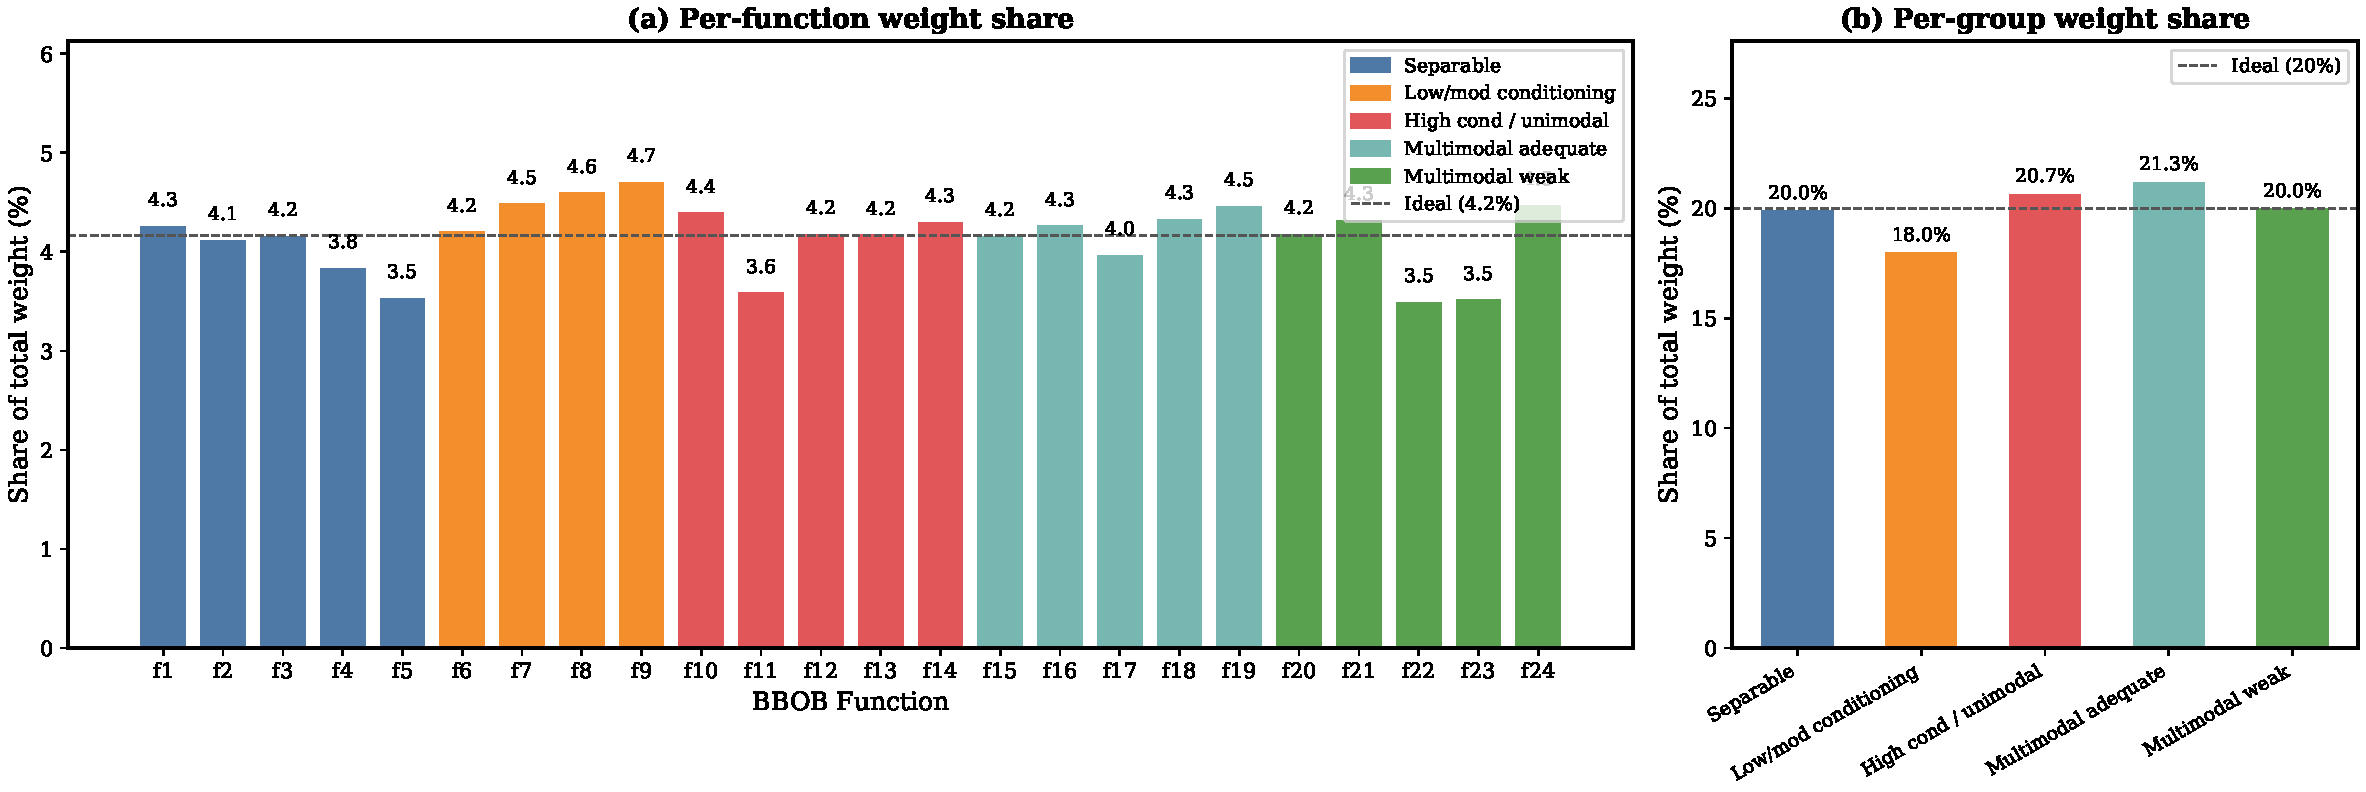
\includegraphics[width=\textwidth]{figures/fig_mabbob_instances_phase4.pdf}
  \caption{Per-BBOB-function (left) and per-group (right) weight distribution of the 20 MA-BBOB functions used in Stage~4. Dashed lines mark the ideal uniform shares (4.2\% per BBOB function, 20\% per group). All 24 BBOB functions are covered, with a coefficient of variation of $0.080$ across per-BBOB-function totals and group shares within $\pm$1.3\% of the ideal.}
  \label{fig:mabbob-instances-phase4}
\end{figure*}

\begin{table*}[!t]
\centering
\caption{BBOB function weights for the 20 MA-BBOB functions used in Stage~4. Values are percentages of total weight; empty cells indicate zero weight.}
\label{tab:instance-weights-phase4}
\scriptsize
\begin{tabular}{@{}r|cccccccccccccccccccccccc@{}}
\toprule
\textbf{Func.} & \textbf{1} & \textbf{2} & \textbf{3} & \textbf{4} & \textbf{5} & \textbf{6} & \textbf{7} & \textbf{8} & \textbf{9} & \textbf{10} & \textbf{11} & \textbf{12} & \textbf{13} & \textbf{14} & \textbf{15} & \textbf{16} & \textbf{17} & \textbf{18} & \textbf{19} & \textbf{20} & \textbf{21} & \textbf{22} & \textbf{23} & \textbf{24} \\
\midrule
22  &    & 18 &    &    & 7  & 13 &    &    & 18 &    &    & 15 & 3  &    &    &    &    &    & 12 &    &    & 13 &    &    \\
93  &    &    &    &    &    &    &    &    & 19 &    & 16 &    & 23 &    &    &    &    & 18 & 20 &    &    &    & 4  &    \\
166 &    &    &    &    &    &    &    &    &    &    &    &    &    & 15 & 17 &    &    & 23 &    & 30 &    &    &    & 15 \\
196 & 5  & 19 &    &    & 11 & 10 &    &    &    &    &    &    &    &    & 15 & 11 &    & 4  &    &    & 10 &    &    & 16 \\
203 &    & 30 &    &    & 30 & 18 &    &    &    &    & 22 &    &    &    &    &    &    &    &    &    &    &    &    &    \\
288 &    &    &    & 23 &    &    & 7  &    &    & 27 & 7  &    &    &    &    &    &    &    &    &    & 29 &    & 7  &    \\
321 &    &    &    & 9  &    & 5  & 16 &    & 17 & 10 &    & 18 & 8  &    &    &    & 5  & 12 &    &    &    &    &    &    \\
408 & 24 &    &    & 14 &    &    &    &    &    &    &    &    &    &    &    &    &    & 19 & 20 &    & 22 &    &    &    \\
480 & 19 &    & 22 & 3  &    &    & 6  &    &    &    &    &    &    &    & 8  & 13 &    &    & 10 &    & 18 &    &    &    \\
513 & 15 &    & 27 &    &    &    &    &    &    &    &    &    &    &    &    & 18 &    &    &    & 14 &    &    &    & 26 \\
528 &    &    & 22 &    & 18 &    & 11 &    &    & 3  &    & 12 & 22 &    &    & 10 &    &    &    &    & 1  &    &    &    \\
598 &    &    &    &    &    &    &    & 29 &    &    &    &    &    & 30 &    &    & 27 &    &    & 2  &    &    & 12 &    \\
697 &    &    &    &    &    &    &    & 3  &    & 32 &    & 4  &    & 27 &    & 7  &    &    &    &    & 6  &    & 21 &    \\
781 &    & 15 &    &    &    &    &    &    & 14 &    & 12 &    &    &    &    & 13 & 21 & 10 &    & 15 &    &    &    &    \\
784 &    &    & 12 &    & 5  &    & 12 &    &    &    & 15 & 24 &    &    & 19 &    &    &    &    &    &    & 12 &    &    \\
803 &    &    &    &    &    &    & 21 & 19 &    &    &    &    & 21 &    & 15 & 13 &    &    & 7  & 5  &    &    &    &    \\
894 & 14 &    &    &    &    & 14 &    &    & 16 & 16 &    &    & 6  &    & 10 &    &    &    & 21 &    &    &    &    & 3  \\
947 & 3  &    &    &    &    & 12 & 17 & 18 & 10 &    &    &    &    &    &    &    & 5  &    &    & 17 &    &    &    & 18 \\
951 & 5  &    &    & 3  &    & 12 &    & 11 &    &    &    &    &    &    &    &    & 22 &    &    &    &    & 20 & 27 &    \\
999 &    &    &    & 24 &    &    &    & 13 &    &    &    & 11 &    & 15 &    &    &    & 1  &    &    &    & 25 &    & 12 \\
\bottomrule
\end{tabular}
\end{table*}



\end{document}
